% Manuscript written in the style of an MDPI Remote Sensing research article.
% Build: uv run python report/make_tables.py ; cd report ; pdflatex main ; pdflatex main
\documentclass[10pt,a4paper]{article}
\usepackage[a4paper,left=2.6cm,right=2.6cm,top=2.6cm,bottom=2.4cm,headheight=14pt]{geometry}
\usepackage[T1]{fontenc}
\usepackage{mathpazo}
\usepackage{microtype}
\usepackage{amsmath,amssymb}
\usepackage{graphicx,booktabs,tabularx,array,float,enumitem,pifont,calc}
\usepackage[font=small,labelfont=bf,labelsep=period,justification=justified,singlelinecheck=false]{caption}
\usepackage{subcaption}
\usepackage{xcolor}
\usepackage{fancyhdr,lastpage}
\usepackage{titlesec}
\usepackage[numbers,sort&compress]{natbib}
\usepackage[colorlinks=true,linkcolor=mdpiblue,citecolor=mdpiblue,urlcolor=mdpiblue]{hyperref}
\usepackage[section]{placeins}
\usepackage{tikz}
\usetikzlibrary{positioning,arrows.meta,fit,backgrounds,calc}

\graphicspath{{../figures/notebook/}{../figures/pipeline/}{generated/}}
\newcommand{\dateAsc}{\textcolor{red}{[pending]}}
\newcommand{\dateDesc}{\textcolor{red}{[pending]}}
\newcommand{\geoDRmax}{\textcolor{red}{[pending]}}
\newcommand{\geoDlineMax}{\textcolor{red}{[pending]}}
\newcommand{\geoDpixMax}{\textcolor{red}{[pending]}}
\newcommand{\geoDtMax}{\textcolor{red}{[pending]}}
\newcommand{\geoidN}{\textcolor{red}{[pending]}}
\newcommand{\holesBase}{\textcolor{red}{[pending]}}
\newcommand{\holesNoOver}{\textcolor{red}{[pending]}}
\newcommand{\incAsc}{\textcolor{red}{[pending]}}
\newcommand{\incDesc}{\textcolor{red}{[pending]}}
\newcommand{\kFitDb}{\textcolor{red}{[pending]}}
\newcommand{\nFit}{\textcolor{red}{[pending]}}
\newcommand{\nGrid}{\textcolor{red}{[pending]}}
\newcommand{\nRefitDesc}{\textcolor{red}{[pending]}}
\newcommand{\platAsc}{\textcolor{red}{[pending]}}
\newcommand{\platDesc}{\textcolor{red}{[pending]}}
\newcommand{\rAsc}{\textcolor{red}{[pending]}}
\newcommand{\rDemNinety}{\textcolor{red}{[pending]}}
\newcommand{\rDesc}{\textcolor{red}{[pending]}}
\newcommand{\rDescMu}{\textcolor{red}{[pending]}}
\newcommand{\rNoOver}{\textcolor{red}{[pending]}}
\newcommand{\repoURL}{https://github.com/Vedansh7-7/dem-sar-simulation}
\newcommand{\sceneAsc}{\textcolor{red}{[pending]}}
\newcommand{\sceneDesc}{\textcolor{red}{[pending]}}
\newcommand{\shiftAscL}{\textcolor{red}{[pending]}}
\newcommand{\shiftAscP}{\textcolor{red}{[pending]}}
\newcommand{\shiftNoGeoidP}{\textcolor{red}{[pending]}}
\newcommand{\ssimAsc}{\textcolor{red}{[pending]}}
\newcommand{\ssimDesc}{\textcolor{red}{[pending]}}


% ------------------------------------------------------------------ style
\definecolor{mdpiblue}{HTML}{1E5AA8}
\definecolor{inC}{HTML}{DCE9F5}   \definecolor{inD}{HTML}{2F5F8A}
\definecolor{prC}{HTML}{E3F1E6}   \definecolor{prD}{HTML}{2E7D4A}
\definecolor{reC}{HTML}{F3EAD7}   \definecolor{reD}{HTML}{8A6A2F}
\definecolor{ouC}{HTML}{FBE3D6}   \definecolor{ouD}{HTML}{B5532A}
\definecolor{okC}{HTML}{2E7D32}   \definecolor{noC}{HTML}{C62828}
\newcommand{\ok}{\textcolor{okC}{\ding{51}}}
\newcommand{\no}{\textcolor{noC}{\ding{55}}}
\renewcommand{\bibnumfmt}[1]{#1.}
\setlength{\bibsep}{2pt}
\setlength{\parindent}{1.5em}
\setlength{\parskip}{0pt}
\titleformat{\section}{\normalsize\bfseries}{\thesection.}{0.4em}{}
\let\oldsubsection\subsection\renewcommand{\subsection}{\FloatBarrier\oldsubsection}
\titleformat{\subsection}{\normalsize\itshape}{\thesubsection.}{0.4em}{}
\titleformat{\subsubsection}{\normalsize\itshape}{\thesubsubsection.}{0.4em}{}
\titlespacing*{\section}{0pt}{12pt}{6pt}
\titlespacing*{\subsection}{0pt}{9pt}{4pt}
\pagestyle{fancy}\fancyhf{}
\renewcommand{\headrulewidth}{0pt}
\lhead{\small\itshape DEM-based SAR simulation of Sentinel-1 imagery}
\rhead{\small\thepage{} of \pageref{LastPage}}
\fancypagestyle{first}{\fancyhf{}\renewcommand{\headrulewidth}{0pt}}
\setlist[itemize]{leftmargin=1.6em,itemsep=1pt,topsep=3pt}
\setlist[enumerate]{leftmargin=1.6em,itemsep=1pt,topsep=3pt}
\captionsetup[table]{position=top,skip=4pt}
\newcommand{\sigz}{\sigma^0}
\newcommand{\figw}{\textwidth}

\begin{document}
\thispagestyle{first}
% ================================================================= FRONT MATTER
{\small\itshape B.Tech.\ Minor Project Report}\par\vspace{2pt}
{\raggedright\LARGE\bfseries Simulating Sentinel-1 SAR Imagery of Alpine Terrain from a Digital Elevation Model: A First-Principles Simulator and Its Geometric and Radiometric Assessment over Innsbruck, Austria\par}
\vspace{10pt}
{\large\bfseries Vedansh Shrivastava\par}
\vspace{2pt}
{\small Roll No.\ 230003086\par}
\vspace{4pt}
{\small Supervisor: \textbf{Dr.\ Unmesh Khati}\par}
\vspace{4pt}
{\small Indian Institute of Technology Indore, India\par}
\vspace{10pt}
\noindent\rule{\textwidth}{0.4pt}

\noindent{\small\textbf{Abstract:} Synthetic aperture radar (SAR) images of mountainous terrain are dominated by geometry: foreshortening, layover and radar shadow relocate and redistribute the backscattered energy long before surface properties determine the signal. This paper develops a SAR simulator from first principles and assesses how much of a real Sentinel-1 image of Alpine terrain can be predicted from a digital elevation model (DEM) alone. A raw-signal simulator, verified against theory for point targets (slant-range resolution of 2.66\,m, azimuth resolution of 5.45\,m), distributed scatterers and periodic topography, is used to validate a fast image-domain simulator ($r=0.97$ on a real DEM patch, about 3000 times faster). The image-domain simulator is then driven by the Copernicus GLO-30 DEM and by the orbit, timing and slant-to-ground-range annotation of two Sentinel-1 IW GRD scenes (ascending and descending) over Innsbruck, Austria. The implemented range-Doppler geocoding reproduces the geolocation grid of the products to \geoDpixMax{} pixels in range and \geoDtMax{} ms in azimuth time, provided that the slant-to-ground-range polynomials are applied piece-wise rather than interpolated. Predicted radar shadow coincides with the darkest real pixels (median $-$21.0\,dB, the noise floor) and predicted layover with the brightest ($-$3.5\,dB). A local-incidence-angle law $k\cos^{n}\theta_{loc}$ fitted to the ascending scene ($n=\nFit$) reproduces the real $\sigz$ with a Pearson correlation of \rAsc{} and transfers unchanged to the descending scene ($r=\rDesc$). Land cover explains most of the remaining disagreement: forest is reproduced without bias, whereas built-up areas and bare rock are about 3\,dB brighter and water about 4\,dB darker than predicted. The simulator, the experiment pipeline and a tutorial notebook are openly available.\par}

\vspace{6pt}
\noindent{\small\textbf{Keywords:} SAR simulation; Sentinel-1; digital elevation model; Copernicus DEM; layover; radar shadow; range-Doppler geocoding; backscatter model; Alps\par}
\vspace{4pt}
\noindent\rule{\textwidth}{0.4pt}

% ================================================================= 1
\section{Introduction}
Spaceborne synthetic aperture radar (SAR) systems provide images of the Earth's surface independently of daylight and cloud cover, and the Copernicus Sentinel-1 constellation delivers C-band acquisitions over most land surfaces every few days~\cite{torres2012,moreira2013}. Image formation in a SAR is based on the measurement of range and Doppler history rather than on angular projection~\cite{curlander1991,cumming2005}. In mountainous terrain this side-looking range geometry produces characteristic distortions: slopes facing the radar are compressed into few resolution cells (foreshortening), the top of steep slopes is imaged before their foot (layover), and slopes facing away from the sensor may not be illuminated at all (radar shadow)~\cite{leberl1990,kropatsch1990}. In the Alps these effects affect a large fraction of every scene and make visual interpretation and quantitative use of the backscatter difficult~\cite{gelautz1998}. Figure~\ref{fig:intro} illustrates the three effects on a synthetic mountain profile.

\begin{figure}[htbp]
\centering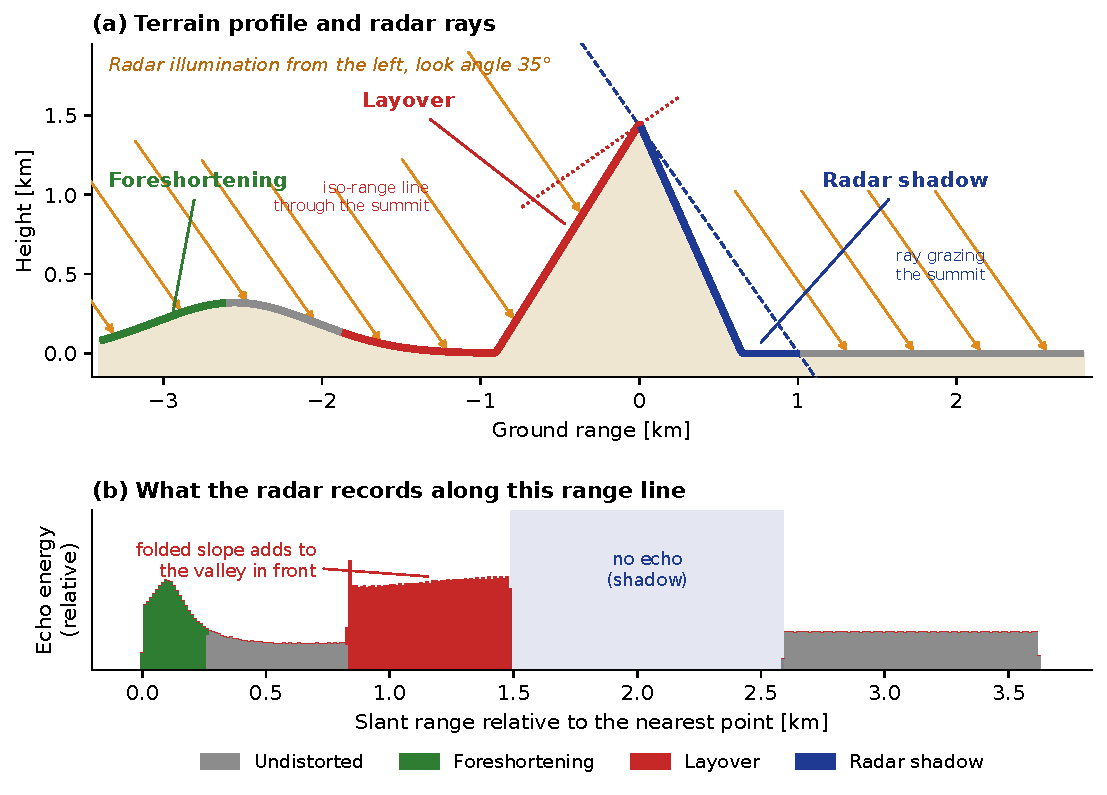
\includegraphics[width=0.92\textwidth]{../figures/intro/sar_distortions.pdf}
\caption{Geometric distortions of a side-looking SAR. (\textbf{a}) Terrain profile illuminated from the left at a look angle of 35$^\circ$: the gentle slope facing the radar is foreshortened, the steep fore-slope and the valley floor in front of it are in layover, and the back-slope and the terrain behind it lie in radar shadow. (\textbf{b}) Echo energy recorded along this range line: the foreshortened slope is compressed and bright, the folded fore-slope is added to the valley floor, and the shadow returns no echo.}
\label{fig:intro}
\end{figure}


Simulating the image that a SAR should record from a DEM is the classical way to understand, predict and correct these effects. DEM-based simulations are used to geocode and terrain-correct SAR data~\cite{schreier1993,meier1993,small2011,low2007}, to generate layover and shadow masks~\cite{kropatsch1990}, to estimate the illuminated area for radiometric normalisation~\cite{ulander1996,small2011,frey2013}, and to co-register images precisely~\cite{nitti2011}. Simulators span a wide range of complexity, from raw-signal simulators that generate the echo of every pulse~\cite{franceschetti1992}, through ray tracers that model multiple bounces in urban scenes~\cite{balz2009,auer2010}, to the image-domain simulators that operational terrain-correction chains rely on~\cite{meier1993,small2011}. The radiometric component of such simulators is commonly reduced to a function of the local incidence angle, such as the cosine law, Lambert's law or Muhleman's law~\cite{muhleman1964,ulaby1982}, whose validity for real terrain remains an empirical question~\cite{ulaby1989}.

Two developments make a fresh assessment timely. First, the Copernicus GLO-30 DEM provides a consistent global elevation model at 1\,arcsec resolution~\cite{copdem}. Second, Sentinel-1 Ground Range Detected (GRD) products are distributed with a complete annotation of orbit state vectors, zero-Doppler timing, slant-to-ground-range (SRGR) polynomials and radiometric calibration~\cite{s1pd}, and are streamed as cloud-optimised files without registration~\cite{planetary}. Their absolute geolocation accuracy has been verified with corner reflectors~\cite{schubert2015,gisinger2021}. Together, they allow a simulation to be computed in the exact geometry of a product and compared with it pixel by pixel. What is less well documented is how far such a DEM-only simulation goes in explaining a real C-band image of high-relief terrain, which processing choices matter, and where the remaining disagreement comes from.

This study addresses this gap. Its objectives are (1) to build a transparent SAR simulator from first principles and verify each of its components quantitatively, from the impulse response of a point target to a real DEM; (2) to drive the simulator with the annotated geometry of real Sentinel-1 GRD products and assess its geometric accuracy against the products' own geolocation; (3) to assess the radiometric agreement with the real images for several backscatter laws, for two viewing geometries and for several processing choices; and (4) to identify, with an independent land-cover map, which part of the image a DEM cannot explain.

The paper is organised as follows. Section~\ref{sec:data} describes the study site and the data. Section~\ref{sec:method} presents the raw-signal and image-domain simulators, the range-Doppler geocoding, the treatment of shadow, layover and radiometry, and the comparison strategy. Section~\ref{sec:results} presents and discusses the results, including the limitations of the study, and Section~\ref{sec:conclusions} draws the conclusions.

% ================================================================= 2
\section{Data and Study Site}
\label{sec:data}
\subsection{Study Site}
The study site (11.25--11.55$^\circ$\,E, 47.15--47.35$^\circ$\,N; approximately $23\times22$\,km$^2$) is centred on the city of Innsbruck in Tyrol, Austria (Figure~\ref{fig:site}). The east--west oriented Inn valley, with a floor at about 580\,m above sea level, separates the steep south face of the Nordkette (up to 2300\,m) in the north from the Patscherkofel and the Stubai pre-Alps in the south; the Sill gorge (Wipptal) enters the valley from the south. Elevations within the site range from 552\,m to 2789\,m. The site therefore contains all regimes of geometric distortion and a strong land-cover contrast between the urbanised valley floor, extensive forests, alpine grassland and bare rock.

\begin{figure}[htbp]
\centering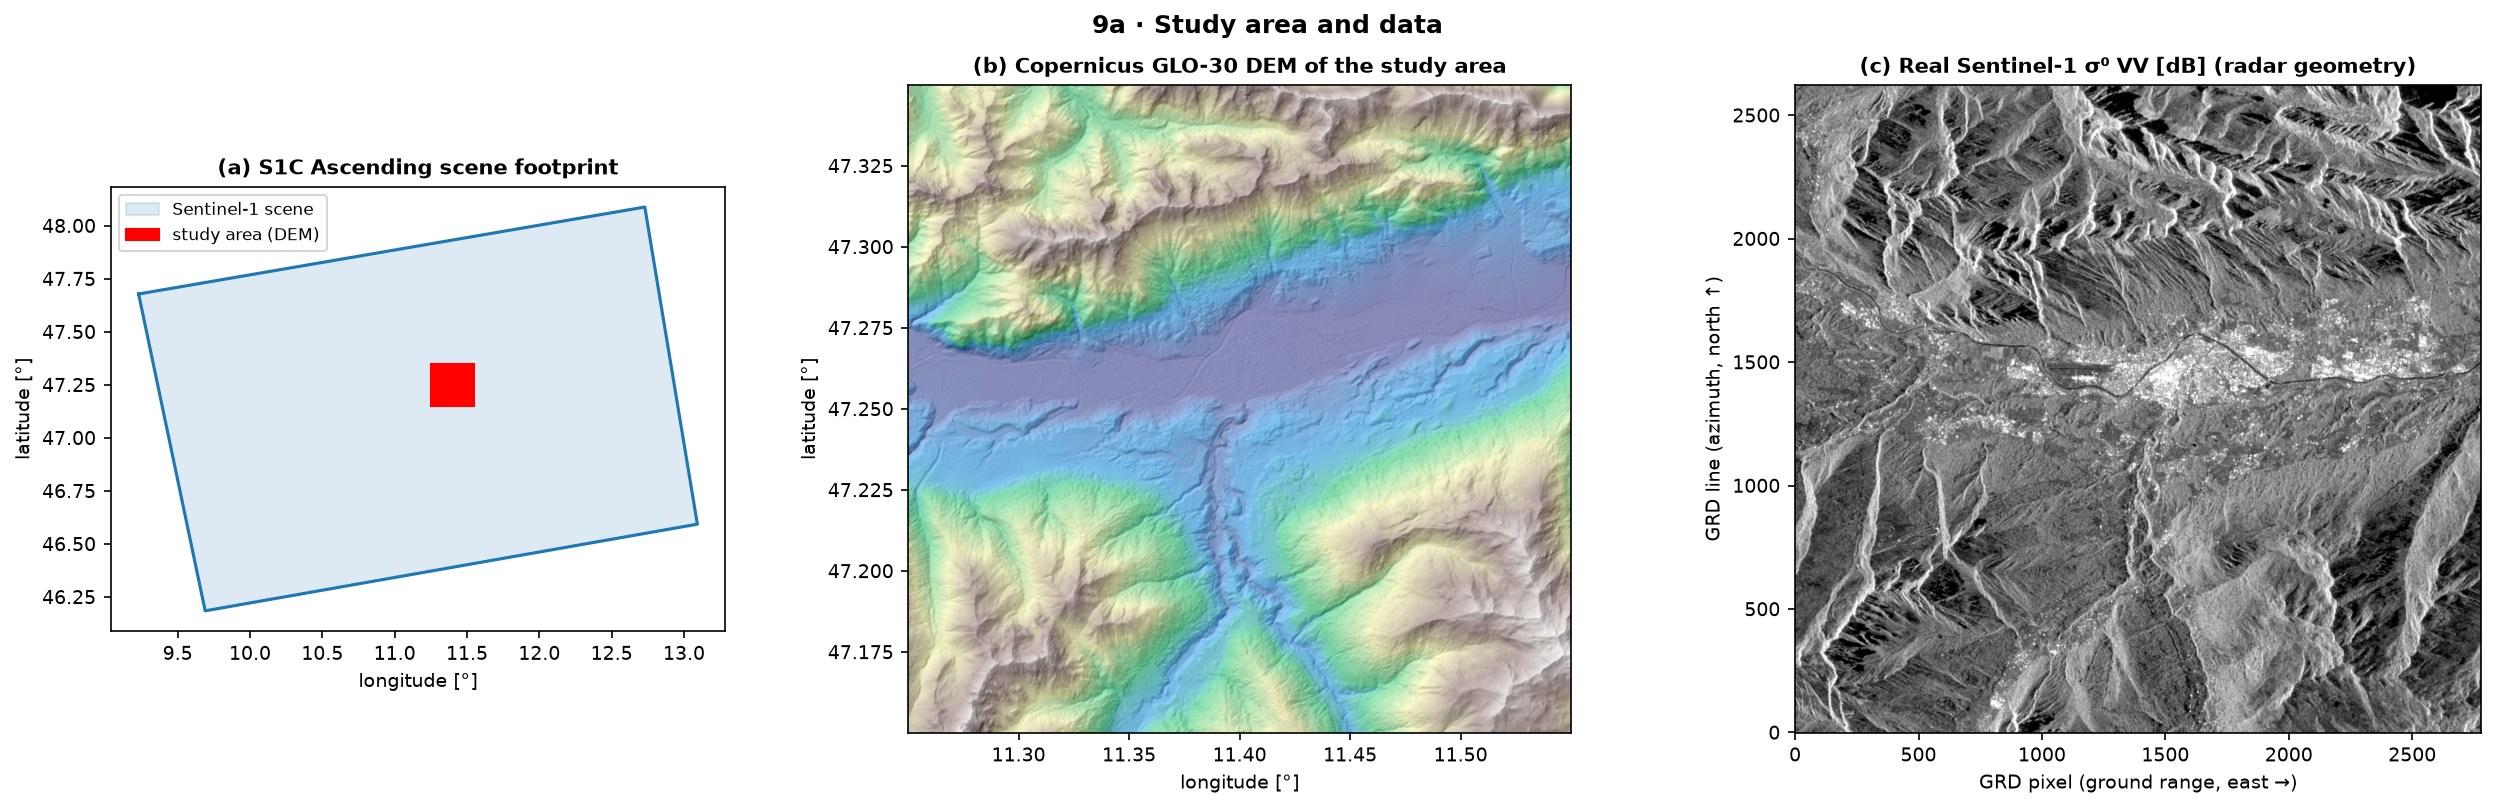
\includegraphics[width=\figw]{09a_study_area_data.png}
\caption{Study site and data. (\textbf{a}) Footprint of the ascending Sentinel-1 scene and the study site (red). (\textbf{b}) Copernicus GLO-30 DEM of the study site. (\textbf{c}) Calibrated Sentinel-1 $\sigz$ (VV) of the study site in radar geometry.}
\label{fig:site}
\end{figure}

\subsection{Digital Elevation Model}
The Copernicus GLO-30 DEM~\cite{copdem} tile N47\,E011 was cropped to the study site, yielding $720\times1080$ samples at 1\,arcsec spacing (about 31\,m north--south and 21\,m east--west). GLO-30 heights refer to the EGM2008 geoid~\cite{pavlis2012}; they were converted to WGS84 ellipsoidal heights with the geoid undulation $N=\geoidN$\,m obtained from the EGM2008 model, as required by the orbit-based geocoding.

\subsection{Sentinel-1 Data}
Two Sentinel-1C Interferometric Wide-swath (IW) GRD high-resolution products in VV polarisation, one from an ascending and one from a descending pass, were selected as the most recent scenes in August--September 2025 that fully cover the site (Table~\ref{tab:s1}). The ascending pass looks east and the descending pass looks west, so that the two geometries illuminate opposite slopes. Only the window of each GRD image that covers the DEM (about $2600\times2780$ pixels of $10\times10$\,m) was read from the cloud-optimised file. For each product, the annotation provides the orbit state vectors (10\,s spacing), the zero-Doppler time of the first line and the azimuth time interval, 28 time-tagged SRGR polynomials, the geolocation grid (210 tie points) and the radiometric calibration look-up table~\cite{s1pd}.

\begin{table}[htbp]
\caption{Sentinel-1 data used in this study. Incidence angle at mid-swath; window size in GRD pixels.}
\label{tab:s1}
\centering\small
\begin{tabularx}{\textwidth}{lXX}
\toprule
 & \textbf{Ascending} & \textbf{Descending}\\\midrule
Platform, mode, polarisation & \platAsc, IW GRDH, VV & \platDesc, IW GRDH, VV\\
Acquisition start (UTC) & \dateAsc, 17:06:22 & \dateDesc, 05:17:54\\
Absolute orbit & 4313 & 4291\\
Look direction & east & west\\
Incidence angle (mid-swath) & \incAsc$^\circ$ & \incDesc$^\circ$\\
Pixel spacing (range $\times$ azimuth) & $10\times10$\,m & $10\times10$\,m\\
Window covering the DEM & $2622\times2780$ & $2600\times2772$\\
\bottomrule
\end{tabularx}
\end{table}

\subsection{Land Cover}
The ESA WorldCover 2021 map at 10\,m resolution~\cite{worldcover} was sampled at the DEM grid by nearest-neighbour interpolation. Within the analysed area, tree cover represents 55\,\% of the pixels, grassland 26\,\%, built-up areas 7\,\%, bare or sparsely vegetated land 6\,\% and cropland 4\,\%; water, snow and ice, and moss and lichen together represent about 2\,\%. All data sets were accessed through the Microsoft Planetary Computer~\cite{planetary}.

% ================================================================= 3
\section{Methodology}
\label{sec:method}
The simulator was developed incrementally, from a single point target to a full Sentinel-1 scene. Each stage had to pass a quantitative test before the next stage was built, and the tests that failed determined the design decisions of the final processing chain (Figure~\ref{fig:design}). The final data flow is summarised in Figure~\ref{fig:dataflow}.

\subsection{Raw-Signal Simulator}
\label{sec:raw}
To verify the physics of the simulation, a raw-signal simulator was implemented for a sensor with Sentinel-1-like parameters (wavelength $\lambda=5.55$\,cm, chirp bandwidth $B=50$\,MHz, pulse length $T_p=10\,\mu$s, sampling rate 60\,MHz, antenna length $L=12.3$\,m, pulse repetition frequency 1700\,Hz) flying a straight track at 693\,km altitude with a look angle of 35$^\circ$ over a flat Earth. The transmitted pulse is the linear frequency-modulated chirp
\begin{equation}
s(t)=\exp\!\left(j\pi K_r t^2\right),\qquad |t|<T_p/2,\qquad K_r=B/T_p .
\end{equation}
For a set of point scatterers with complex reflectivity $a_i$ at positions $\mathbf{P}_i$, the echo received at slow time $\eta$ is
\begin{equation}
e(t,\eta)=\sum_i a_i\,G\!\left(\vartheta_i(\eta)\right)\,s\!\left(t-\frac{2R_i(\eta)}{c}\right)\exp\!\left(-j\frac{4\pi R_i(\eta)}{\lambda}\right),
\label{eq:raw}
\end{equation}
where $R_i(\eta)$ is the range from the sensor to scatterer $i$ and $G$ is the two-way azimuth antenna pattern $\mathrm{sinc}^2(L\vartheta/\lambda)$ of the squint angle $\vartheta$. Equation~(\ref{eq:raw}) is evaluated efficiently by placing a band-limited impulse at the exact fractional delay of each scatterer and convolving with the chirp in the frequency domain. Range compression is performed by matched filtering with the chirp replica, and azimuth compression by time-domain back-projection,
\begin{equation}
I(\mathbf{x})=\sum_{\eta} s_{rc}\!\left(\frac{2R(\mathbf{x},\eta)}{c},\eta\right)\exp\!\left(j\frac{4\pi R(\mathbf{x},\eta)}{\lambda}\right),
\end{equation}
which is exact for arbitrary scene geometry and therefore also displaces elevated points towards the sensor when the image is formed on a flat reference plane. The simulator was verified on a single point target, on lines of targets, on three targets observed along the synthetic aperture, on fields of randomly distributed scatterers (speckle), on a sinusoidal surface and on a $480\times480$\,m patch of the Copernicus DEM (Section~\ref{sec:res-verif}).

\subsection{Image-Domain Simulator}
Because generating raw data for millions of scatterers is impractical, scene-scale simulations use an image-domain simulator: every DEM facet is projected directly to its zero-Doppler position (azimuth time, slant range), its backscattered power is accumulated in the image grid and, for comparison with focused raw-signal simulations, blurred with the impulse response measured in Section~\ref{sec:res-verif}. The equivalence of the two approaches was verified on the sinusoidal surface and on the DEM patch.

\subsection{Range-Doppler Geocoding in Sentinel-1 GRD Geometry}
For the real scenes, the orbit state vectors within $\pm90$\,s of the scene are fitted with a polynomial of degree 7 per ECEF coordinate; its derivative reproduces the annotated velocities to 0.1\,mm/s. For a ground point $\mathbf{X}$, the zero-Doppler azimuth time $t$ solves
\begin{equation}
f(t)=\left(\mathbf{X}-\mathbf{S}(t)\right)\cdot\mathbf{V}(t)=0,
\label{eq:zd}
\end{equation}
where $\mathbf{S}$ and $\mathbf{V}$ are the sensor position and velocity. Equation~(\ref{eq:zd}) is solved by Newton iteration with $f'(t)=-|\mathbf{V}|^2+(\mathbf{X}-\mathbf{S})\cdot\mathbf{A}$; eight iterations reach machine precision. The GRD line is $t/\Delta t_{az}$, with $t$ measured from the first image line. The slant range $R=|\mathbf{X}-\mathbf{S}(t)|$ is converted to ground range with the annotated SRGR polynomial
\begin{equation}
g(R)=\sum_{k=0}^{8}c_k\,(R-R_0)^k ,
\end{equation}
and the GRD pixel is $g/\Delta_{gr}$. The annotation lists one polynomial set per second of azimuth time. Interpolating linearly between consecutive sets, an apparently natural choice, produced range errors of up to 3.3 pixels with respect to the geolocation grid of the product, because consecutive sets differ by up to 19 pixels. Applying each set from its time tag until the next one (``valid-from'' rule) removes this error (Section~\ref{sec:res-geo}).

\subsection{DEM Facets, Local Incidence Angle, Shadow and Layover}
The ellipsoidal DEM is oversampled three times by bilinear interpolation (about $10\times7$\,m facets, smaller than a GRD pixel) and converted to ECEF coordinates. Facet normals $\hat{\mathbf{n}}$ and true facet areas $A$ follow from the cross product of the grid tangent vectors, and the local incidence angle from $\cos\theta_{loc}=-\hat{\mathbf{u}}\cdot\hat{\mathbf{n}}$, with $\hat{\mathbf{u}}$ the unit look vector. To detect shadow and layover, facets are sorted along each azimuth line by their ground position $\psi$ (geocentric angle from the sensor). A facet is in shadow if a facet closer to the ground track is seen under a larger off-nadir angle $\alpha$, and in layover if a closer facet has a larger slant range or a farther facet a smaller one:
\begin{equation}
\mathrm{shadow}:\ \alpha<\max_{\psi'<\psi}\alpha',\qquad \mathrm{layover}:\ R<\max_{\psi'<\psi}R' \ \ \lor\ \ R>\min_{\psi'>\psi}R' .
\end{equation}
The grouped running extrema are computed in one vectorised pass. For the 7.0 million facets of a scene, the geometry is computed in blocks of DEM rows and stored in single precision (about 34 bytes per facet), which keeps the memory footprint at about 240\,MB.

\subsection{Radiometric Model}
Each illuminated facet contributes $\sigz(\theta_{loc})\,A$ to the four GRD pixels surrounding its fractional (line, pixel) position by bilinear splatting, and the sum is divided by the ellipsoid pixel area $\Delta_{az}\Delta_{gr}$. The simulated image is therefore in the same unit as ESA-calibrated $\sigz$, which refers to the ellipsoid~\cite{small2011}. Five backscatter laws were compared: a constant law, which retains only the illuminated-area term; the cosine law $\sigz\propto\cos\theta_{loc}$; Lambert's law $\sigz\propto\cos^2\theta_{loc}$~\cite{ulaby1982}; Muhleman's law~\cite{muhleman1964},
\begin{equation}
\sigz(\theta_{loc})=0.0133\,\frac{\cos\theta_{loc}}{\left(\sin\theta_{loc}+0.1\cos\theta_{loc}\right)^3},
\end{equation}
and a law $\sigz=k\cos^{n}\theta_{loc}$ fitted to the real image. The fit is a least-squares regression of the median real $\sigz$ (in dB) in 2$^\circ$ bins of $\theta_{loc}$ between 5$^\circ$ and 80$^\circ$, excluding layover and shadow, on $10\log_{10}\cos\theta_{loc}$.

\subsection{Comparison with Sentinel-1}
Real digital numbers were calibrated to $\sigz=\mathrm{DN}^2/A_\sigma^2$ with the bilinearly interpolated calibration table; thermal noise was not removed. Real and simulated images were multilooked with a $5\times5$ boxcar ($50\times50$\,m) and converted to dB. The simulation was co-registered to the real image by sub-pixel cross-correlation within the largest fully valid interior box of the footprint, and its absolute level was calibrated by a single constant, the median difference between real and simulated $\sigz$ in dB. Agreement is reported as the Pearson correlation $r$ and the Spearman correlation $\rho$ over all valid pixels, the structural similarity index (SSIM)~\cite{wang2004} within the interior box, and the root mean square difference (RMSE) after level calibration. For analyses in map geometry, the real image is back-geocoded to the DEM grid using the facet positions.

\subsection{Experimental Design}
The following experiments were carried out (Figure~\ref{fig:dataflow}):
\begin{itemize}
\item E1, backscatter laws: the five laws are applied to the same ascending geometry.
\item E2, second viewing geometry: the law fitted on the ascending scene is applied, unchanged, to the descending scene, which acts as an independent validation.
\item E3, geometric validation: the geocoding is compared with the geolocation grid of both products, and the real $\sigz$ is analysed inside the predicted shadow, layover and foreshortening classes.
\item E4, sensitivity: the simulation is repeated without geoid correction, without DEM oversampling and with a 90\,m DEM obtained by $3\times3$ aggregation of GLO-30.
\item E5, land cover: the residual (real minus simulated) is analysed per WorldCover class in map geometry.
\end{itemize}

\begin{figure}[htbp]
\centering
% Data flow of the simulator (shared style with the A3 poster)
\begin{tikzpicture}[yscale=0.92,
  font=\fontsize{7.4}{8.6}\selectfont, >={Stealth[length=1.9mm]},
  base/.style={draw, rounded corners=1.1mm, align=center, minimum height=7.6mm, inner sep=1mm, line width=0.6pt},
  inp/.style={base, fill=inC, draw=inD, text width=19mm},
  pro/.style={base, fill=prC, draw=prD, text width=27mm},
  rea/.style={base, fill=reC, draw=reD, text width=27mm},
  prod/.style={base, fill=ouC, draw=ouD, text width=27mm, font=\fontsize{7.4}{8.6}\selectfont\bfseries},
  ar/.style={->, line width=0.6pt, draw=black!70},
  fb/.style={->, line width=0.75pt, draw=ouD, dashed}]
\def\xA{0mm} \def\xB{47mm} \def\xC{94mm}
\node[inp, text width=18mm] (dem) at (\xA,0) {Copernicus\\GLO-30 DEM};
\node[inp, text width=18mm] (geo) at (23mm,0) {EGM2008\\geoid};
\node[inp, text width=24mm] (ann) at (\xB+1mm,0) {S1 annotation\\{\fontsize{6.4}{7.2}\selectfont orbit, timing, SRGR, LUT}};
\node[inp, text width=19mm] (grd) at (\xC-6mm,0) {S1 GRD image\\(DN, VV)};
\node[inp, text width=16mm] (wc) at (\xC+21mm,0) {ESA\\WorldCover};
\node[pro] (hgt)  at (\xA,-11mm) {ellipsoidal heights\\$h=H+N$};
\node[pro] (orb)  at (\xB,-11mm) {orbit polynomial fit\\{\fontsize{6.4}{7.2}\selectfont velocity error 0.1\,mm/s}};
\node[rea] (cal)  at (\xC,-11mm) {calibration\\$\sigma^0=\mathrm{DN}^2/A_\sigma^2$};
\node[pro] (ovs)  at (\xA,-21.5mm) {3$\times$ oversampling\\{\fontsize{6.4}{7.2}\selectfont about 10\,m facets}};
\node[pro] (zd)   at (\xB,-21.5mm) {zero-Doppler solve\\$(\mathbf X-\mathbf S)\cdot\mathbf V=0$};
\node[rea] (rml)  at (\xC,-21.5mm) {real $\sigma^0$\\5$\times$5 multilook};
\node[pro] (ecef) at (\xA,-32mm) {ECEF facets\\normal $\hat{\mathbf n}$, area $A$};
\node[pro] (srgr) at (\xB,-32mm) {slant range to pixel\\{\fontsize{6.4}{7.2}\selectfont piece-wise SRGR}};
\node[pro] (inc)  at (\xA,-43mm) {local incidence $\theta_{loc}$\\shadow \& layover};
\node[pro] (spl)  at (\xB,-43mm) {$\sigma^0(\theta_{loc})\,A$ splatted\\over pixel area};
\node[pro] (reg)  at (\xC,-43mm) {sub-pixel\\co-registration};
\node[pro] (fit)  at (\xA,-54mm) {fit $\sigma^0=k\cos^n\theta_{loc}$\\{\fontsize{6.4}{7.2}\selectfont to the real image}};
\node[prod] (sim) at (\xB,-54mm) {SIMULATED $\sigma^0$\\+ layover/shadow masks};
\node[prod] (met) at (\xC,-54mm) {metrics\\$r$, $\rho$, SSIM, RMSE};
\node[pro]  (map) at (\xB,-65mm) {back-geocode to map,\\per-class residuals};
\node[prod] (res) at (\xC,-65mm) {residual maps,\\land-cover bias};
\draw[ar] (dem) -- (hgt);
\draw[ar] (geo.south) |- ($(hgt.north east)+(-3mm,1.8mm)$) -- ++(0,-1.8mm);
\draw[ar] (hgt) -- (ovs);
\draw[ar] (ovs) -- (ecef);
\draw[ar] (ann) -- (orb);
\draw[ar] (orb) -- (zd);
\draw[ar] (zd) -- (srgr);
\draw[ar] (ecef.east) -- ++(3mm,0) |- (zd.west);
\draw[ar] (ecef) -- (inc);
\draw[ar] (srgr) -- (spl);
\draw[ar] (inc) -- (spl);
\draw[ar] (spl) -- (sim);
\draw[ar] (grd.south) -- ++(0,-2mm) -| (cal.north);
\draw[ar] (ann.east) -- ++(2mm,0) |- ($(cal.west)+(0,1.5mm)$);
\draw[ar] (cal) -- (rml);
\draw[ar] (rml) -- (reg);
\draw[ar] (sim.north east) -- (reg.south west);
\draw[ar] (reg) -- (met);
\draw[ar] (sim) -- (map);
\draw[ar] (map) -- (res);
\draw[ar] (wc.south) |- (res.east);
\draw[fb] (map.west) -| (fit.south);
\draw[fb] (fit.north) -- (inc.south);
\node[font=\fontsize{7}{8}\selectfont\bfseries\color{black!50}, anchor=south west] at ($(dem.north west)+(0,0.5mm)$) {INPUTS};
\begin{scope}[on background layer]
  \node[fill=black!3.5, rounded corners=2mm, fit=(hgt)(ovs)(ecef), inner sep=1.3mm] {};
  \node[fill=black!3.5, rounded corners=2mm, fit=(orb)(zd)(srgr), inner sep=1.3mm] {};
  \node[fill=reC!45, rounded corners=2mm, fit=(cal)(rml), inner sep=1.3mm] {};
\end{scope}
\end{tikzpicture}

\caption{Data flow of the simulator. Blue: inputs; green: simulation; beige: real-image path; orange: products. The dashed loop fits the backscatter law to the real image and feeds it back into the simulation.}
\label{fig:dataflow}
\vspace{8mm}
% Design evolution of the simulator (shared style with the A3 poster)
\begin{tikzpicture}[font=\fontsize{7.3}{8.4}\selectfont, >={Stealth[length=1.7mm]},
  st/.style={draw=prD, fill=prC, rounded corners=1mm, line width=0.6pt, text width=38mm, minimum height=6mm, align=left, inner sep=1mm},
  te/.style={draw=inD, fill=inC, rounded corners=1mm, line width=0.6pt, text width=27mm, minimum height=6mm, align=left, inner sep=1mm},
  okb/.style={draw=okC, fill=okC!7, rounded corners=1mm, line width=0.6pt, text width=60mm, minimum height=6mm, align=left, inner sep=1mm},
  nob/.style={draw=noC, fill=noC!6, rounded corners=1mm, line width=0.6pt, text width=60mm, minimum height=6mm, align=left, inner sep=1mm},
  ar/.style={->, line width=0.55pt, draw=black!60}]
\def\dy{7.6mm}
\foreach \i/\stage/\test/\res/\kind in {
  1/{\textbf{1}\ \ Point target, one pulse}/{$-3$\,dB width vs theory}/{\ok\ 2.66\,m measured = $0.886\,c/2B$}/okb,
  2/{\textbf{2}\ \ Moving satellite, focusing}/{resolution, side-lobes}/{\ok\ $\rho_{az}$ 5.45\,m, $\rho_g$ 4.65\,m, PSLR $-13$\,dB}/okb,
  3/{\textbf{3}\ \ Speckle \& sine surface}/{image-domain vs raw}/{\ok\ exponential speckle; profiles agree, $r=0.90$}/okb,
  4/{\textbf{4}\ \ Real DEM patch}/{speed \& agreement}/{\ok\ 100\,s vs 30\,ms, $r=0.97$; chosen: \textbf{image-domain}}/okb,
  5/{\textbf{5}\ \ Real orbit, zero-Doppler}/{vs ESA's own grid}/{\no\ 3.3\,px; fix: \textbf{piece-wise SRGR}, 0.016\,px \ok}/nob,
  6/{\textbf{6}\ \ Facets into GRD pixels}/{empty pixels}/{\no\ 46\,\% empty; fix: \textbf{3$\times$ DEM oversampling}, 0.01\,\% \ok}/nob,
  7/{\textbf{7}\ \ Terrain heights}/{geoid off vs on}/{\no\ 58\,m shift; fix: \textbf{EGM2008 geoid correction} \ok}/nob,
  8/{\textbf{8}\ \ Full scene, 7\,M facets}/{memory}/{\no\ out of memory; fix: \textbf{block-wise float32} \ok}/nob,
  9/{\textbf{9}\ \ Backscatter law}/{5 laws; asc. vs desc.}/{\ok\ $k\cos^{\nFit}\theta_{loc}$, $r$ = \rAsc\,/\,\rDesc\ \textbf{(cross-validated)}}/okb}{
  \node[st] (s\i) at (0,-\i*\dy) {\stage};
  \node[te, right=2.4mm of s\i] (t\i) {\test};
  \node[\kind, right=2.4mm of t\i] (r\i) {\res};
  \draw[ar] (s\i) -- (t\i);
  \draw[ar] (t\i) -- (r\i);
}
\foreach \i [count=\j from 2] in {1,...,8} { \draw[ar] (s\i) -- (s\j); }
\node[draw=ouD, fill=ouC, line width=0.9pt, rounded corners=1.2mm, align=center, inner sep=1.4mm,
      anchor=north west, font=\fontsize{7.5}{8.8}\selectfont, text width=137mm] (fin) at ($(s9.south west)+(0,-2.8mm)$)
  {\textbf{FINAL DESIGN}\quad image-domain simulator; real orbit and zero-Doppler; piece-wise SRGR; geoid-corrected, 3$\times$ oversampled GLO-30; block-wise float32; fitted $\cos^{n}$ law; co-registration and metrics};
\draw[ar] (s9) -- (s9|-fin.north);
\node[font=\fontsize{7}{8}\selectfont\bfseries\color{black!50}, anchor=south west] at ($(s1.north west)+(0,0.4mm)$) {ITERATION};
\node[font=\fontsize{7}{8}\selectfont\bfseries\color{black!50}, anchor=south west] at ($(t1.north west)+(0,0.4mm)$) {TEST};
\node[font=\fontsize{7}{8}\selectfont\bfseries\color{black!50}, anchor=south west] at ($(r1.north west)+(0,0.4mm)$) {OUTCOME AND DESIGN DECISION};
\end{tikzpicture}

\caption{Design evolution of the simulator. Each iteration had to pass the listed test before the next was built. Green: test passed; red: test failed, and the fix that became part of the final design.}
\label{fig:design}
\end{figure}

% ================================================================= 4
\section{Results and Discussion}
\label{sec:results}
\subsection{Verification of the Simulators}
\label{sec:res-verif}
The single-pulse simulation of a point target (Figure~\ref{fig:point}) reproduces the textbook behaviour of pulse compression: the 10\,$\mu$s echo, about 1.5\,km long in slant range, is compressed into a sinc-shaped peak with a measured $-3$\,dB width of 2.66\,m, equal to the theoretical value $0.886\,c/2B$. Five targets distributed over 160\,m of ground range produce overlapping echoes that are separated after compression, and two targets remain resolved down to a separation of about one ground-range resolution cell of 5.2\,m (Figure~\ref{fig:line}).

\begin{figure}[htbp]
\centering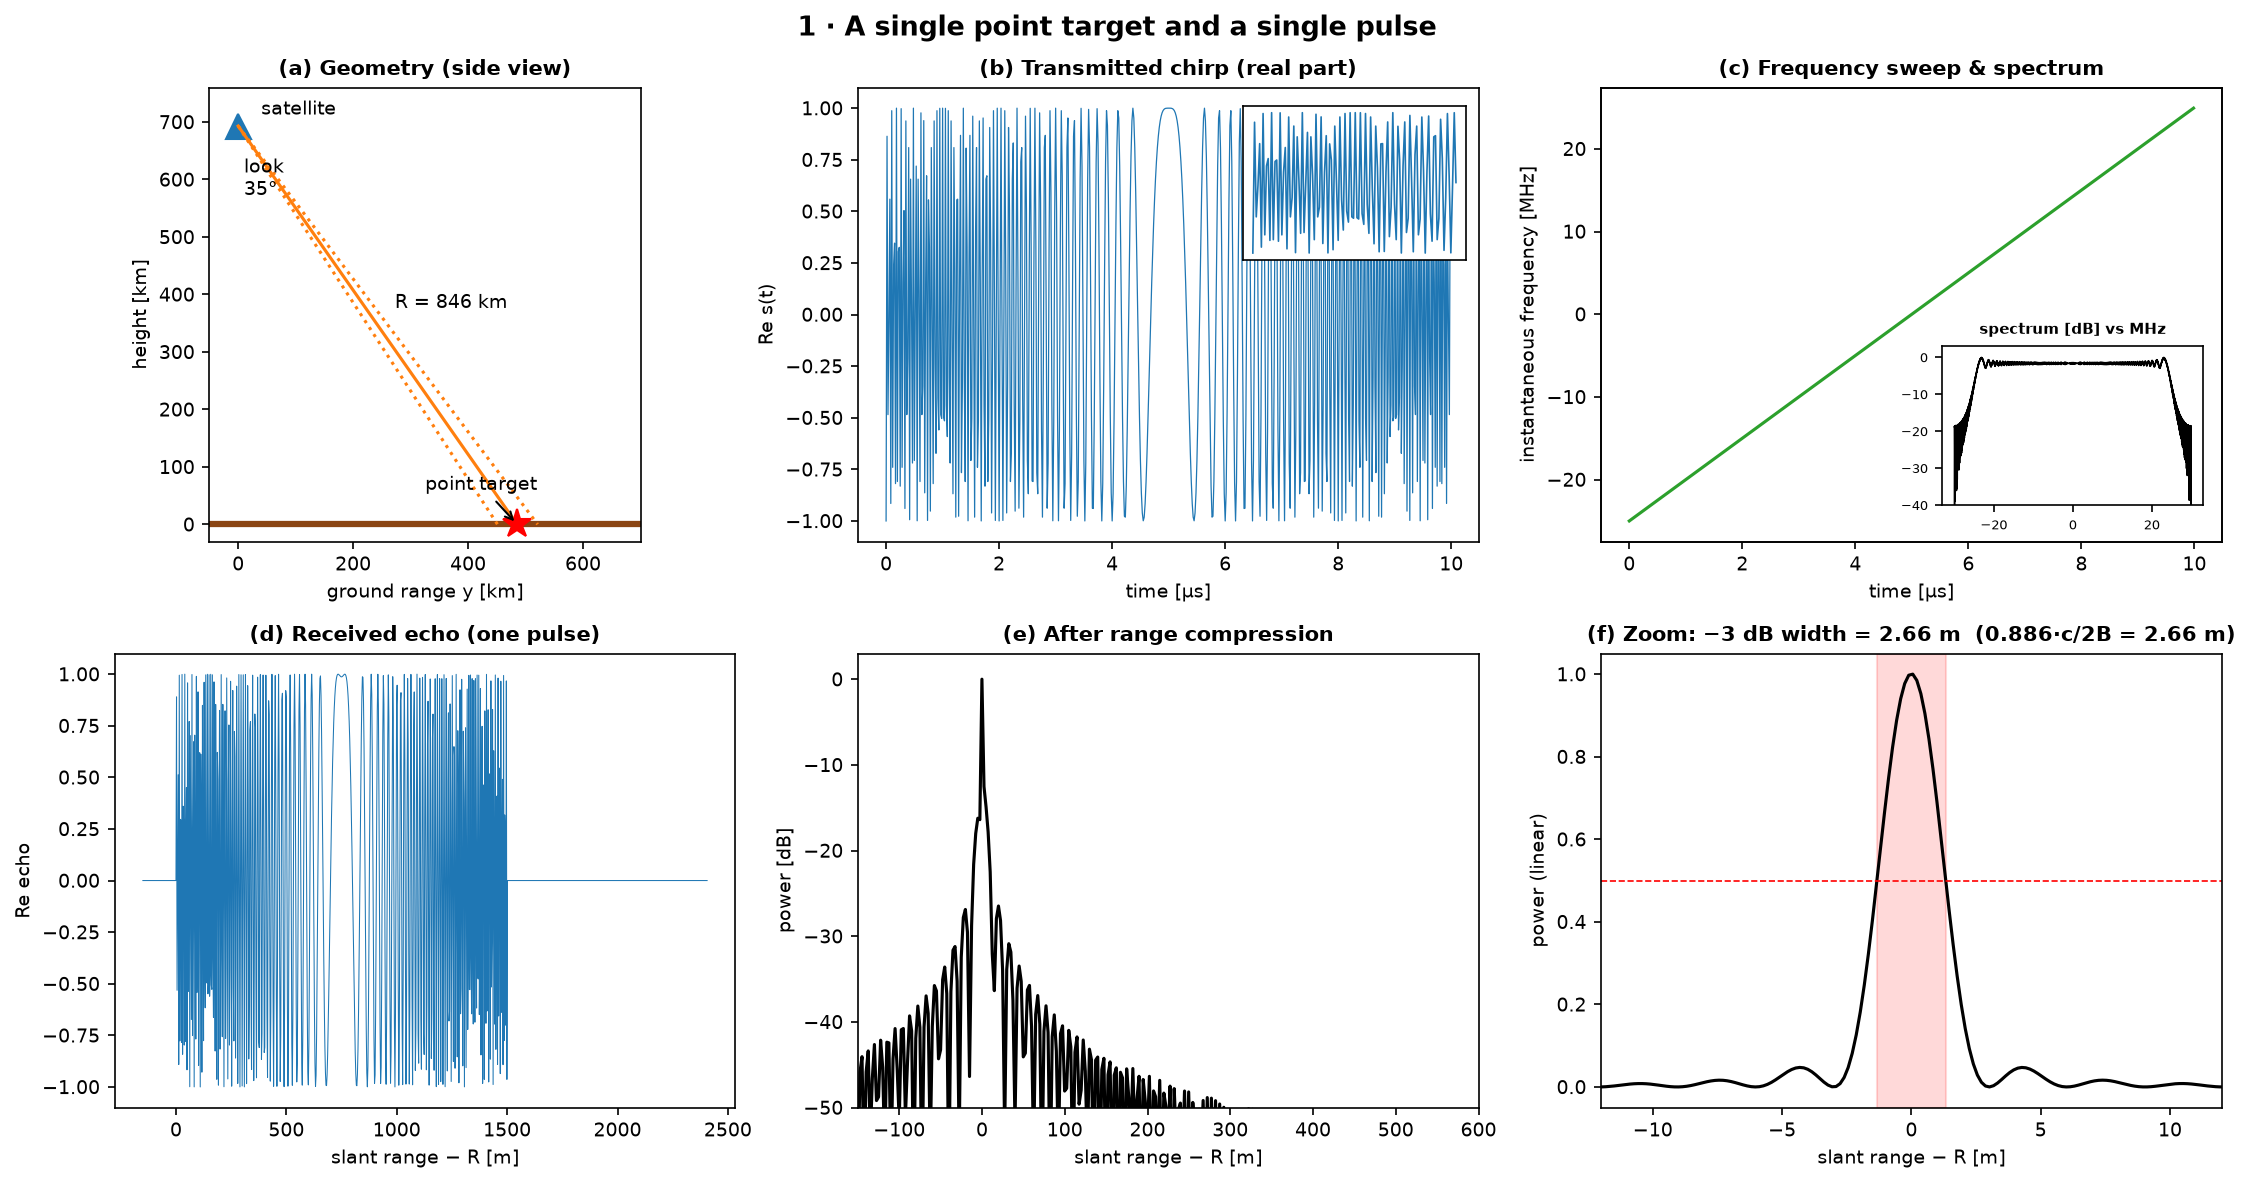
\includegraphics[width=\figw]{01_point_single_pulse.png}
\caption{A single point target illuminated by one pulse: (\textbf{a}) geometry; (\textbf{b}) transmitted chirp; (\textbf{c}) frequency sweep and spectrum; (\textbf{d}) received echo; (\textbf{e}) range-compressed signal; (\textbf{f}) $-3$\,dB width of the compressed peak.}
\label{fig:point}
\end{figure}
\begin{figure}[htbp]
\centering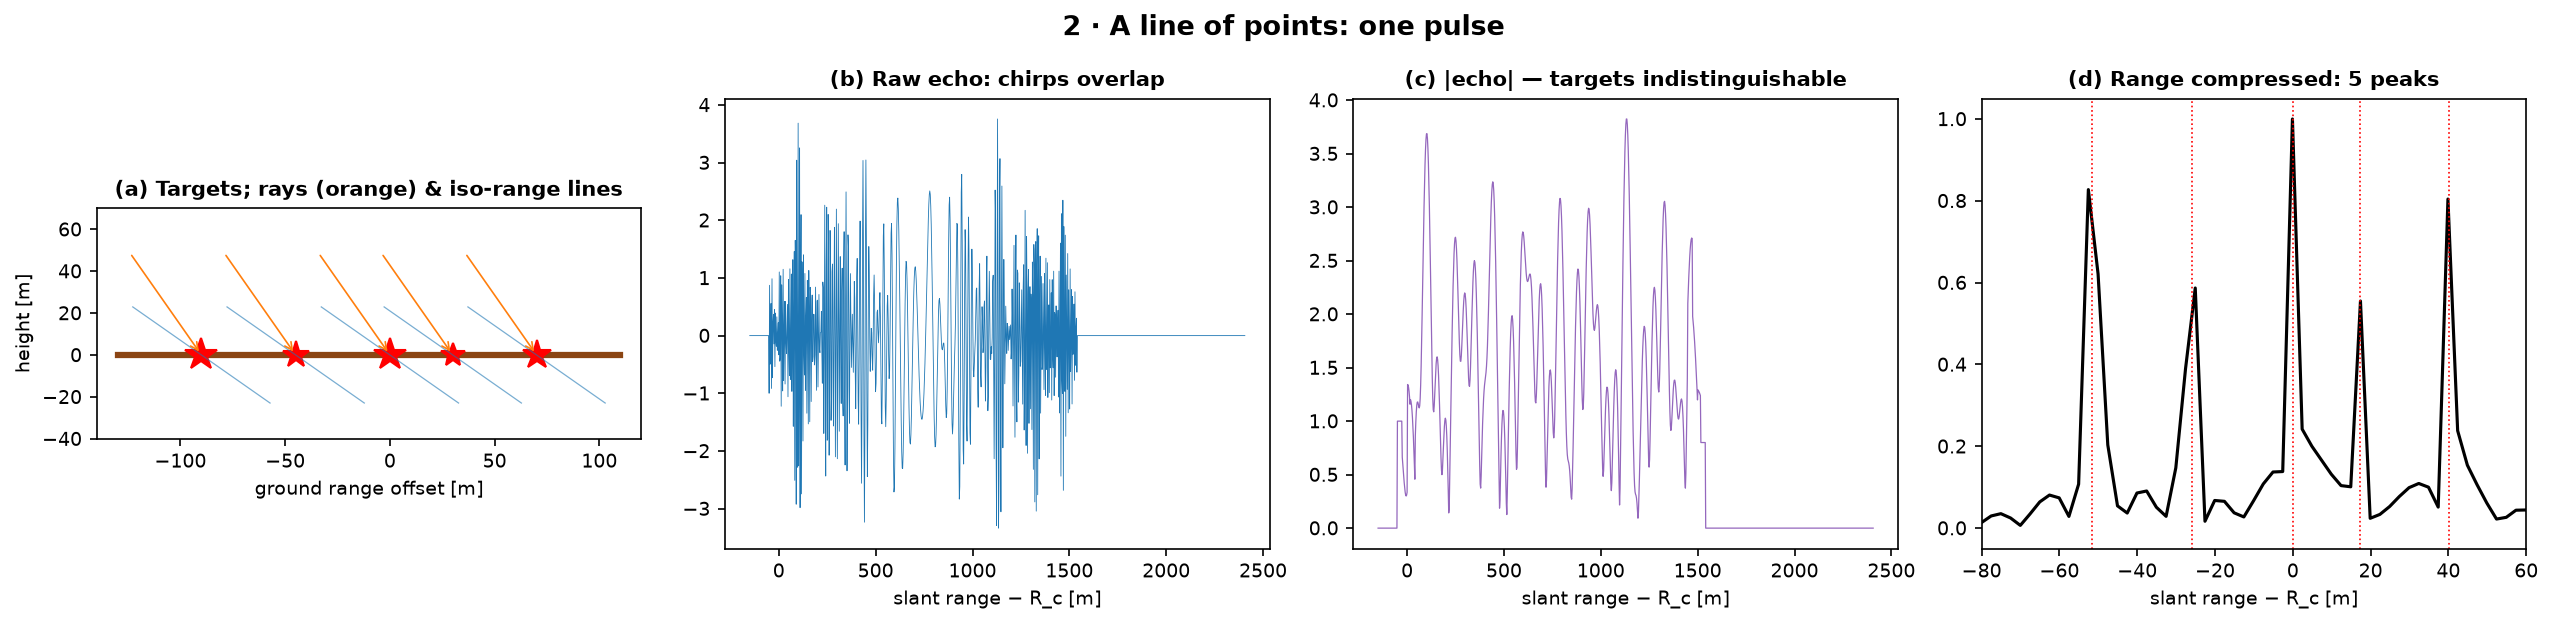
\includegraphics[width=\figw]{02_line_of_points.png}\\[2pt]
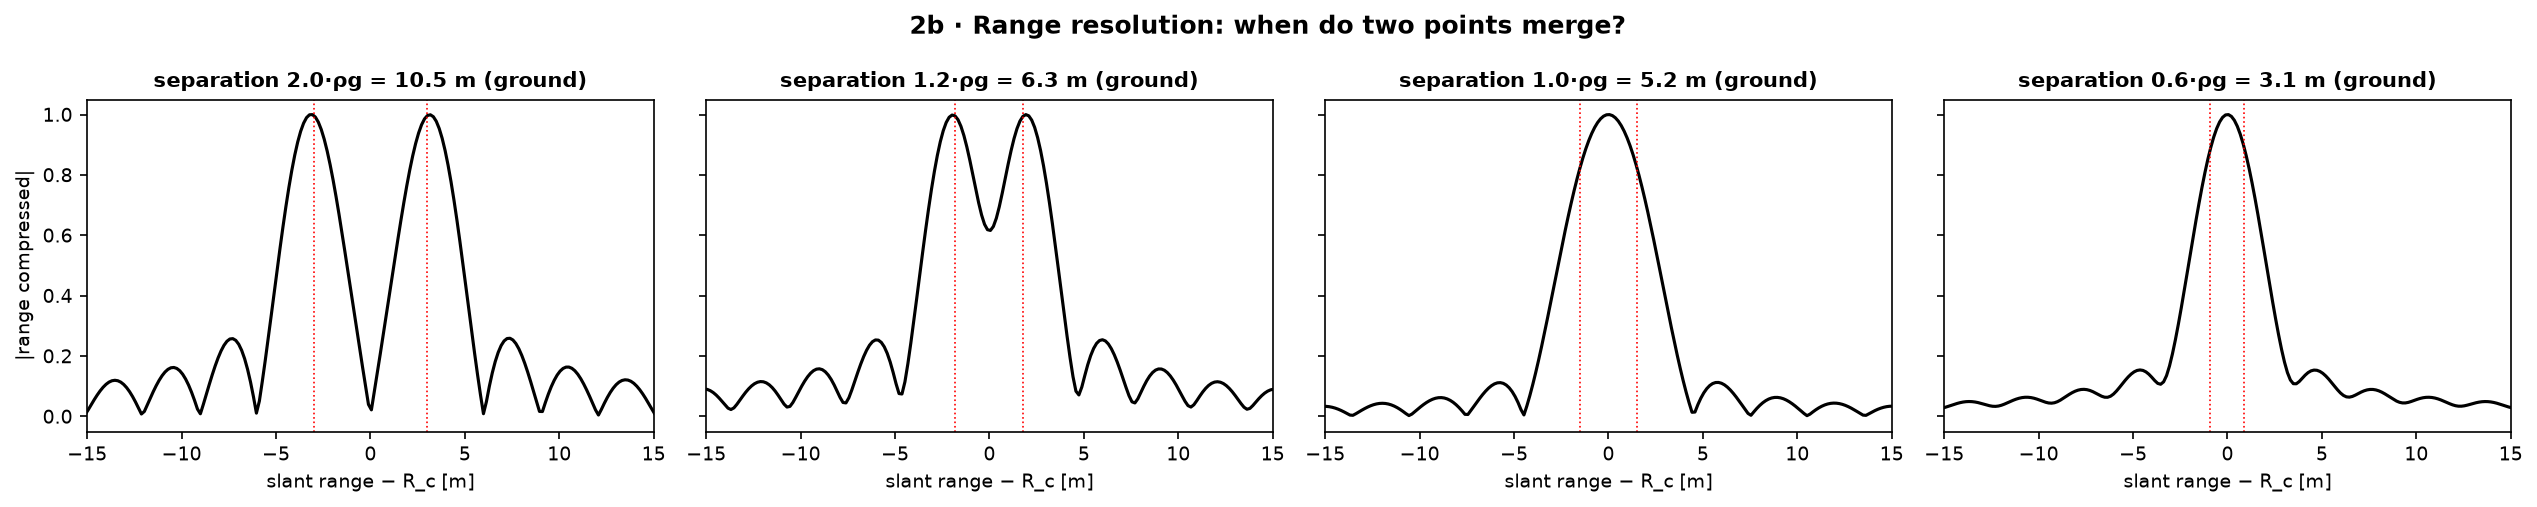
\includegraphics[width=\figw]{02b_range_resolution.png}
\caption{A line of point targets and the range resolution. Top: five targets on a line, their overlapping echoes and the compressed range profile. Bottom: two equal targets at decreasing separation, expressed in multiples of the ground-range resolution $\rho_g$.}
\label{fig:line}
\end{figure}

Along the synthetic aperture, each target follows a hyperbolic range history and a linear Doppler history (Figure~\ref{fig:moving}). For the spaceborne geometry the range migration over the processed aperture of 4.6\,km is only 3.2\,m, about one range resolution cell, so that the range-compressed azimuth chirps are nearly straight. Back-projection focuses the three targets at their true positions with measured resolutions of 5.45\,m in azimuth and 4.65\,m in ground range and peak side-lobe ratios of $-23.6$\,dB and $-13.3$\,dB, respectively (Figure~\ref{fig:irf}); the theoretical values are $L/2=6.15$\,m and $0.886\,\rho_r/\sin\theta=4.63$\,m. The lower azimuth side-lobes result from the antenna pattern, which acts as a taper.

\begin{figure}[htbp]
\centering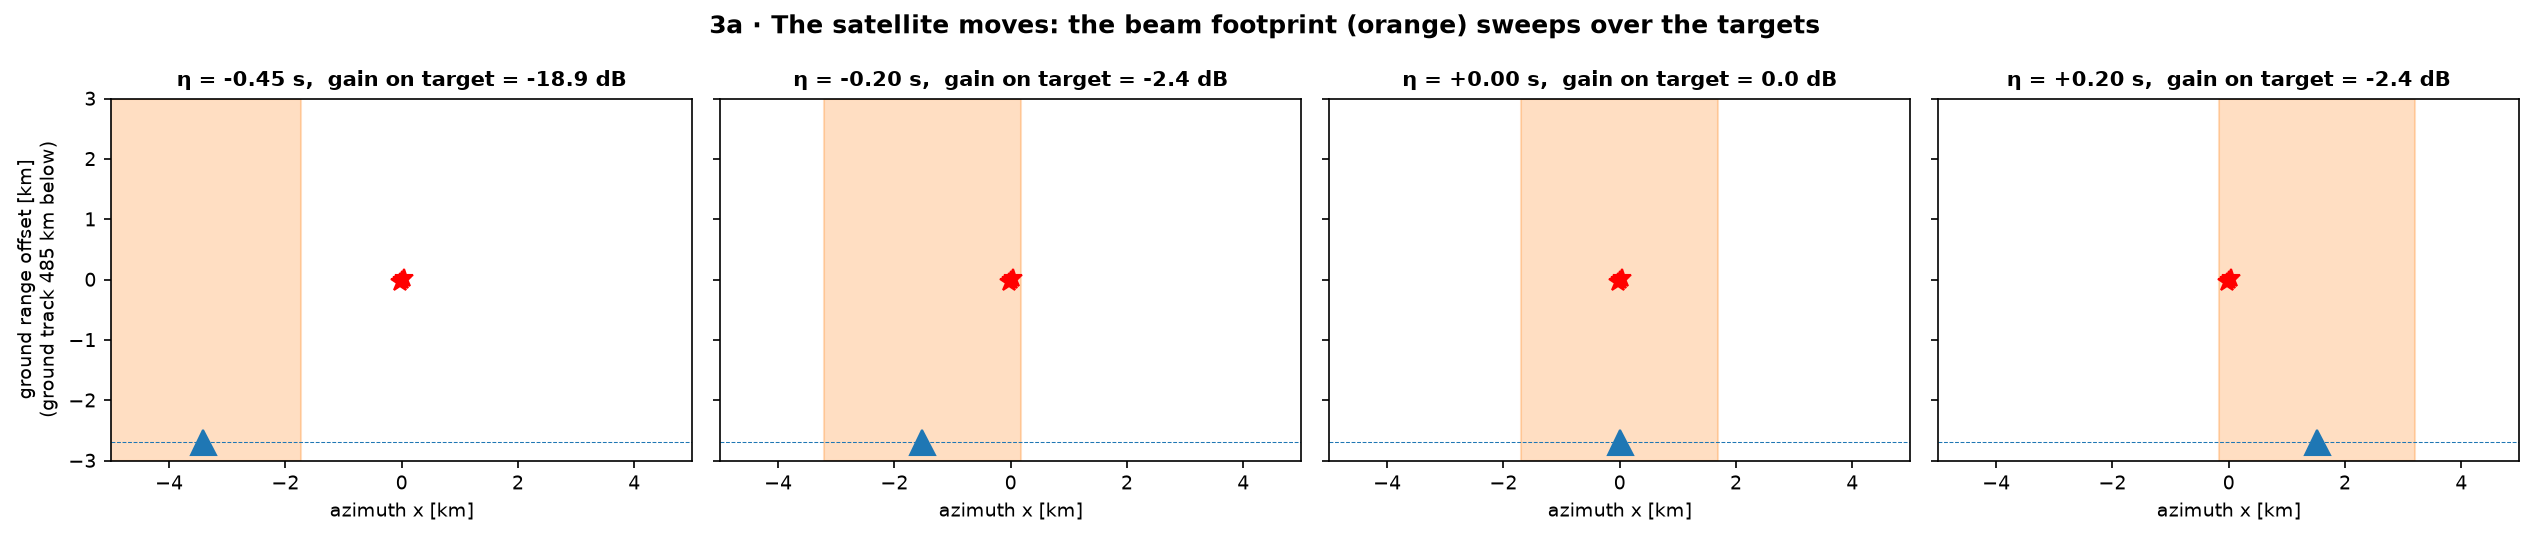
\includegraphics[width=\figw]{03a_moving_satellite_snapshots.png}\\[2pt]
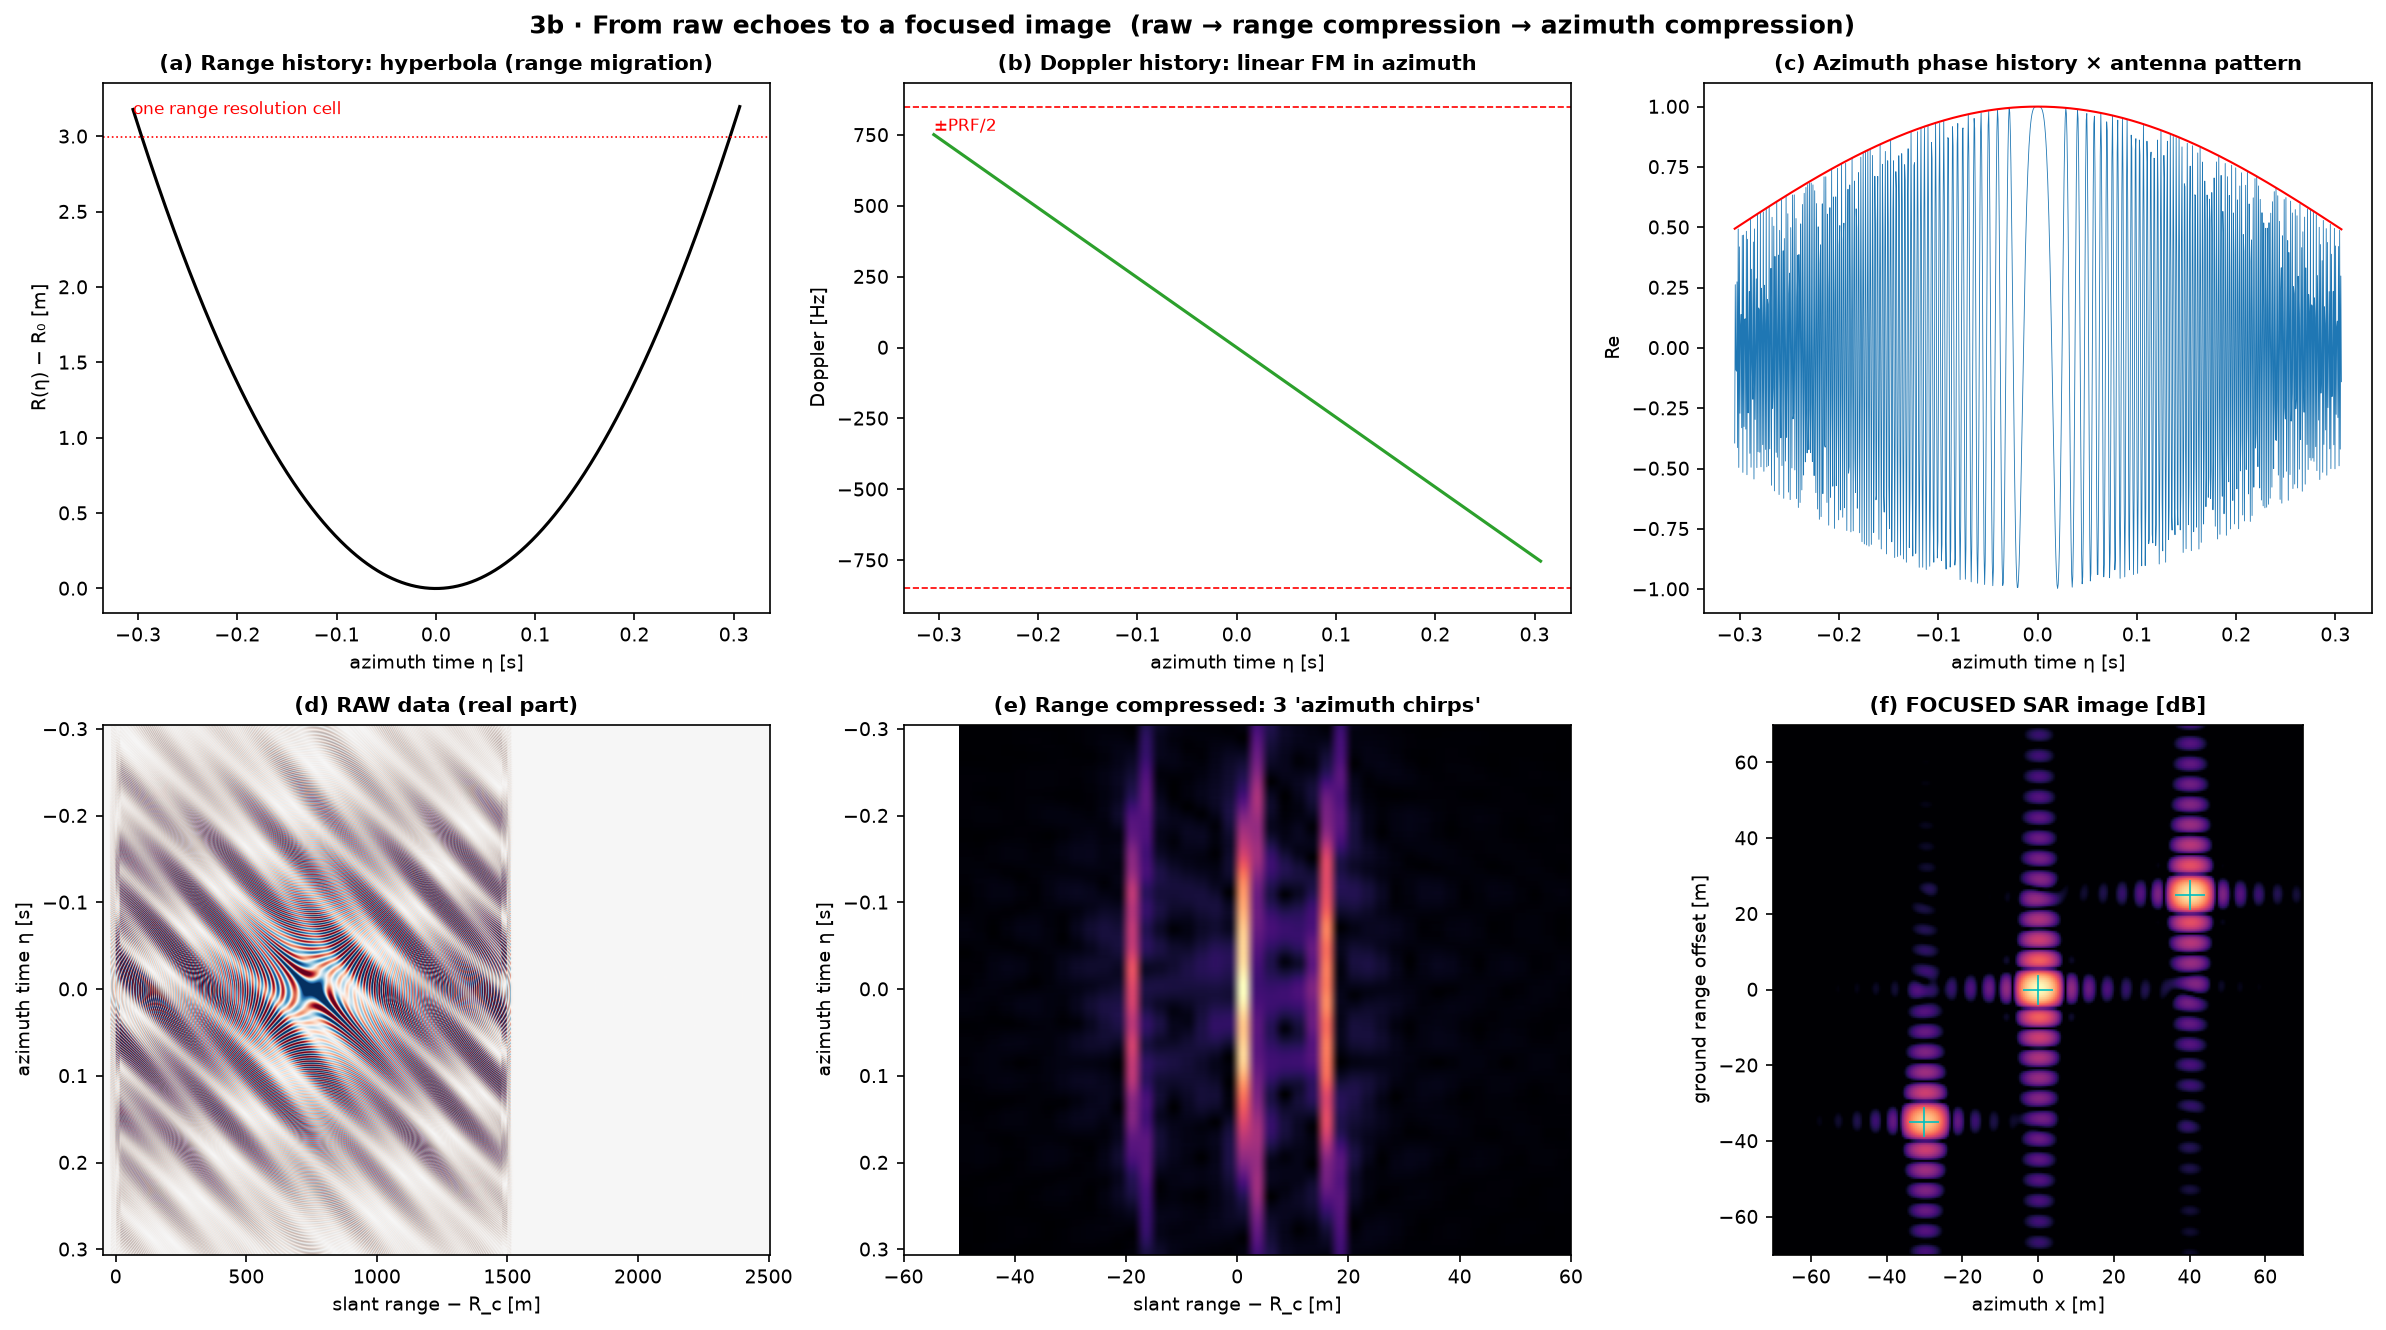
\includegraphics[width=\figw]{03b_signal_chain.png}
\caption{Formation of the synthetic aperture. Top: the beam footprint passing over three targets. Bottom: (\textbf{a}) range history; (\textbf{b}) Doppler history; (\textbf{c}) azimuth phase history weighted by the antenna pattern; (\textbf{d}) raw data; (\textbf{e}) range-compressed data; (\textbf{f}) focused image.}
\label{fig:moving}
\end{figure}
\begin{figure}[htbp]
\centering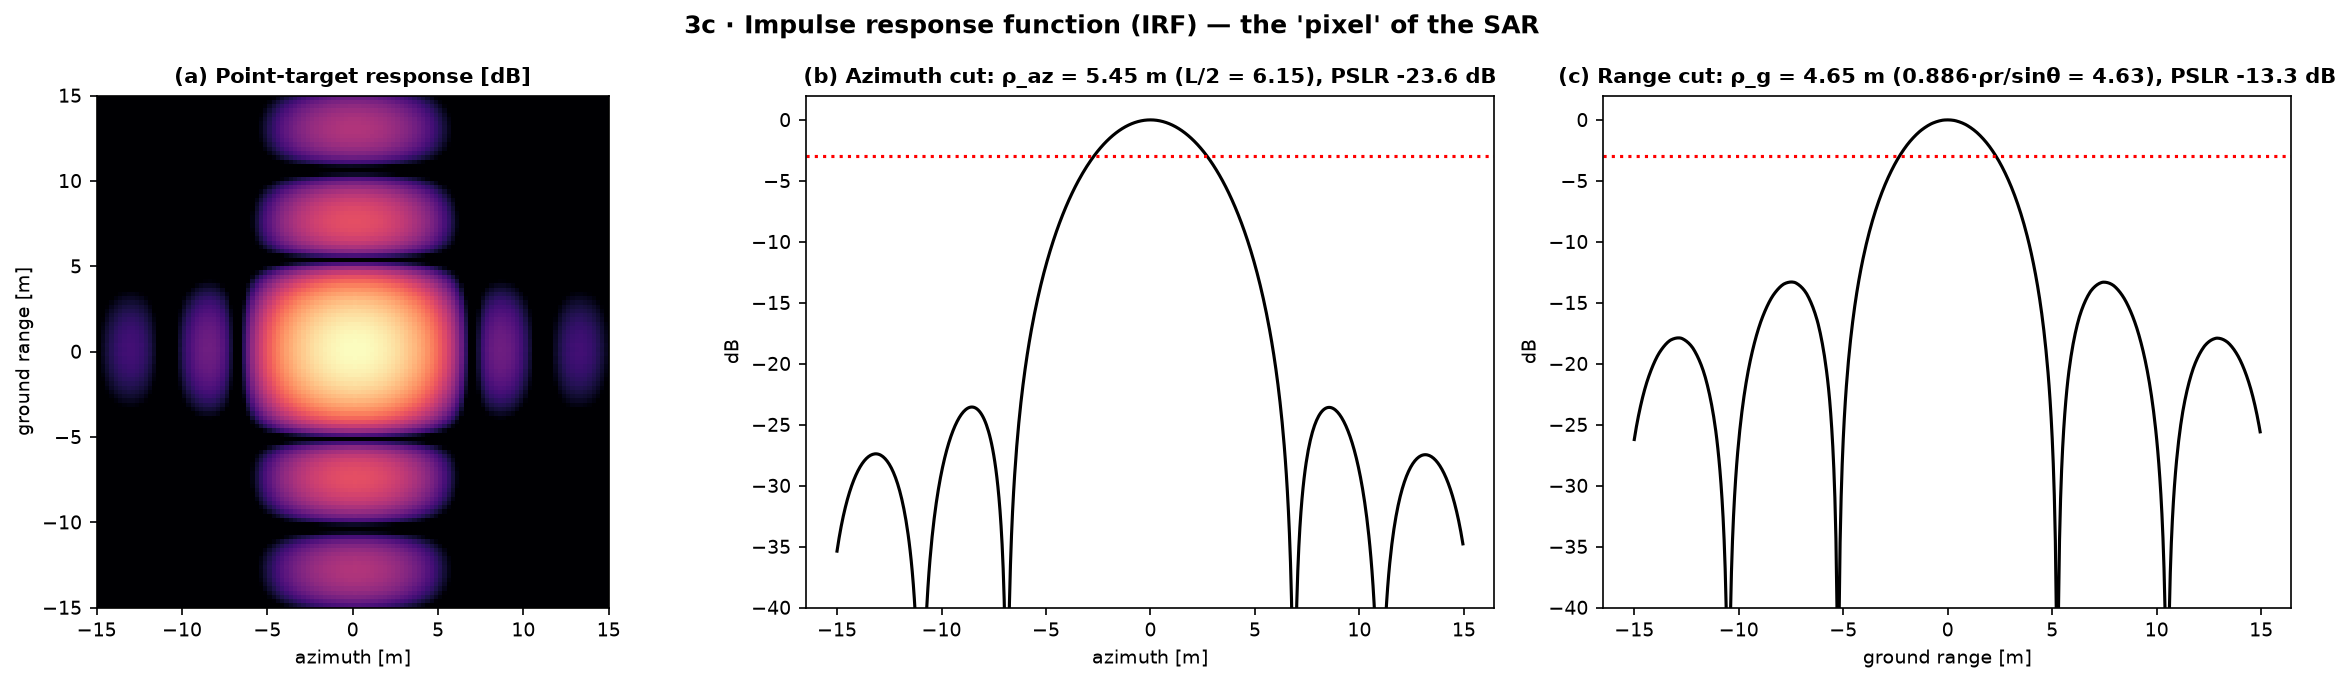
\includegraphics[width=\figw]{03c_impulse_response.png}
\caption{Impulse response function of the simulated SAR (\textbf{a}) and its cuts in azimuth (\textbf{b}) and ground range (\textbf{c}).}
\label{fig:irf}
\end{figure}

A field of 4941 scatterers with circular Gaussian amplitudes produces raw data without visible structure and a focused image that consists of fully developed speckle (Figure~\ref{fig:flat}). The single-look intensity follows the exponential distribution, and multilooking produces a Gamma distribution whose equivalent number of looks agrees with the number of independent resolution cells averaged~\cite{goodman1976,oliver1998}. For a sinusoidal surface with uniform reflectivity per unit ground area (amplitude 12\,m, period 150\,m), the focused image still shows bright bands on the slopes facing the radar (Figure~\ref{fig:sine}); the azimuth-averaged profile of the raw-signal simulation is reproduced by the image-domain simulation with $r=0.90$, the residual being speckle. On the $480\times480$\,m DEM patch (relief of about 550\,m; about 15{,}000 scatterers and 1100 pulses), the raw-signal simulation and focusing take about 100\,s and the image-domain simulation about 30\,ms; after $9\times9$ multilooking both agree with $r=0.97$ (Figure~\ref{fig:dempatch}). The image-domain simulator was therefore adopted for scene-scale simulations (Figure~\ref{fig:design}, iteration 4).

\begin{figure}[htbp]
\centering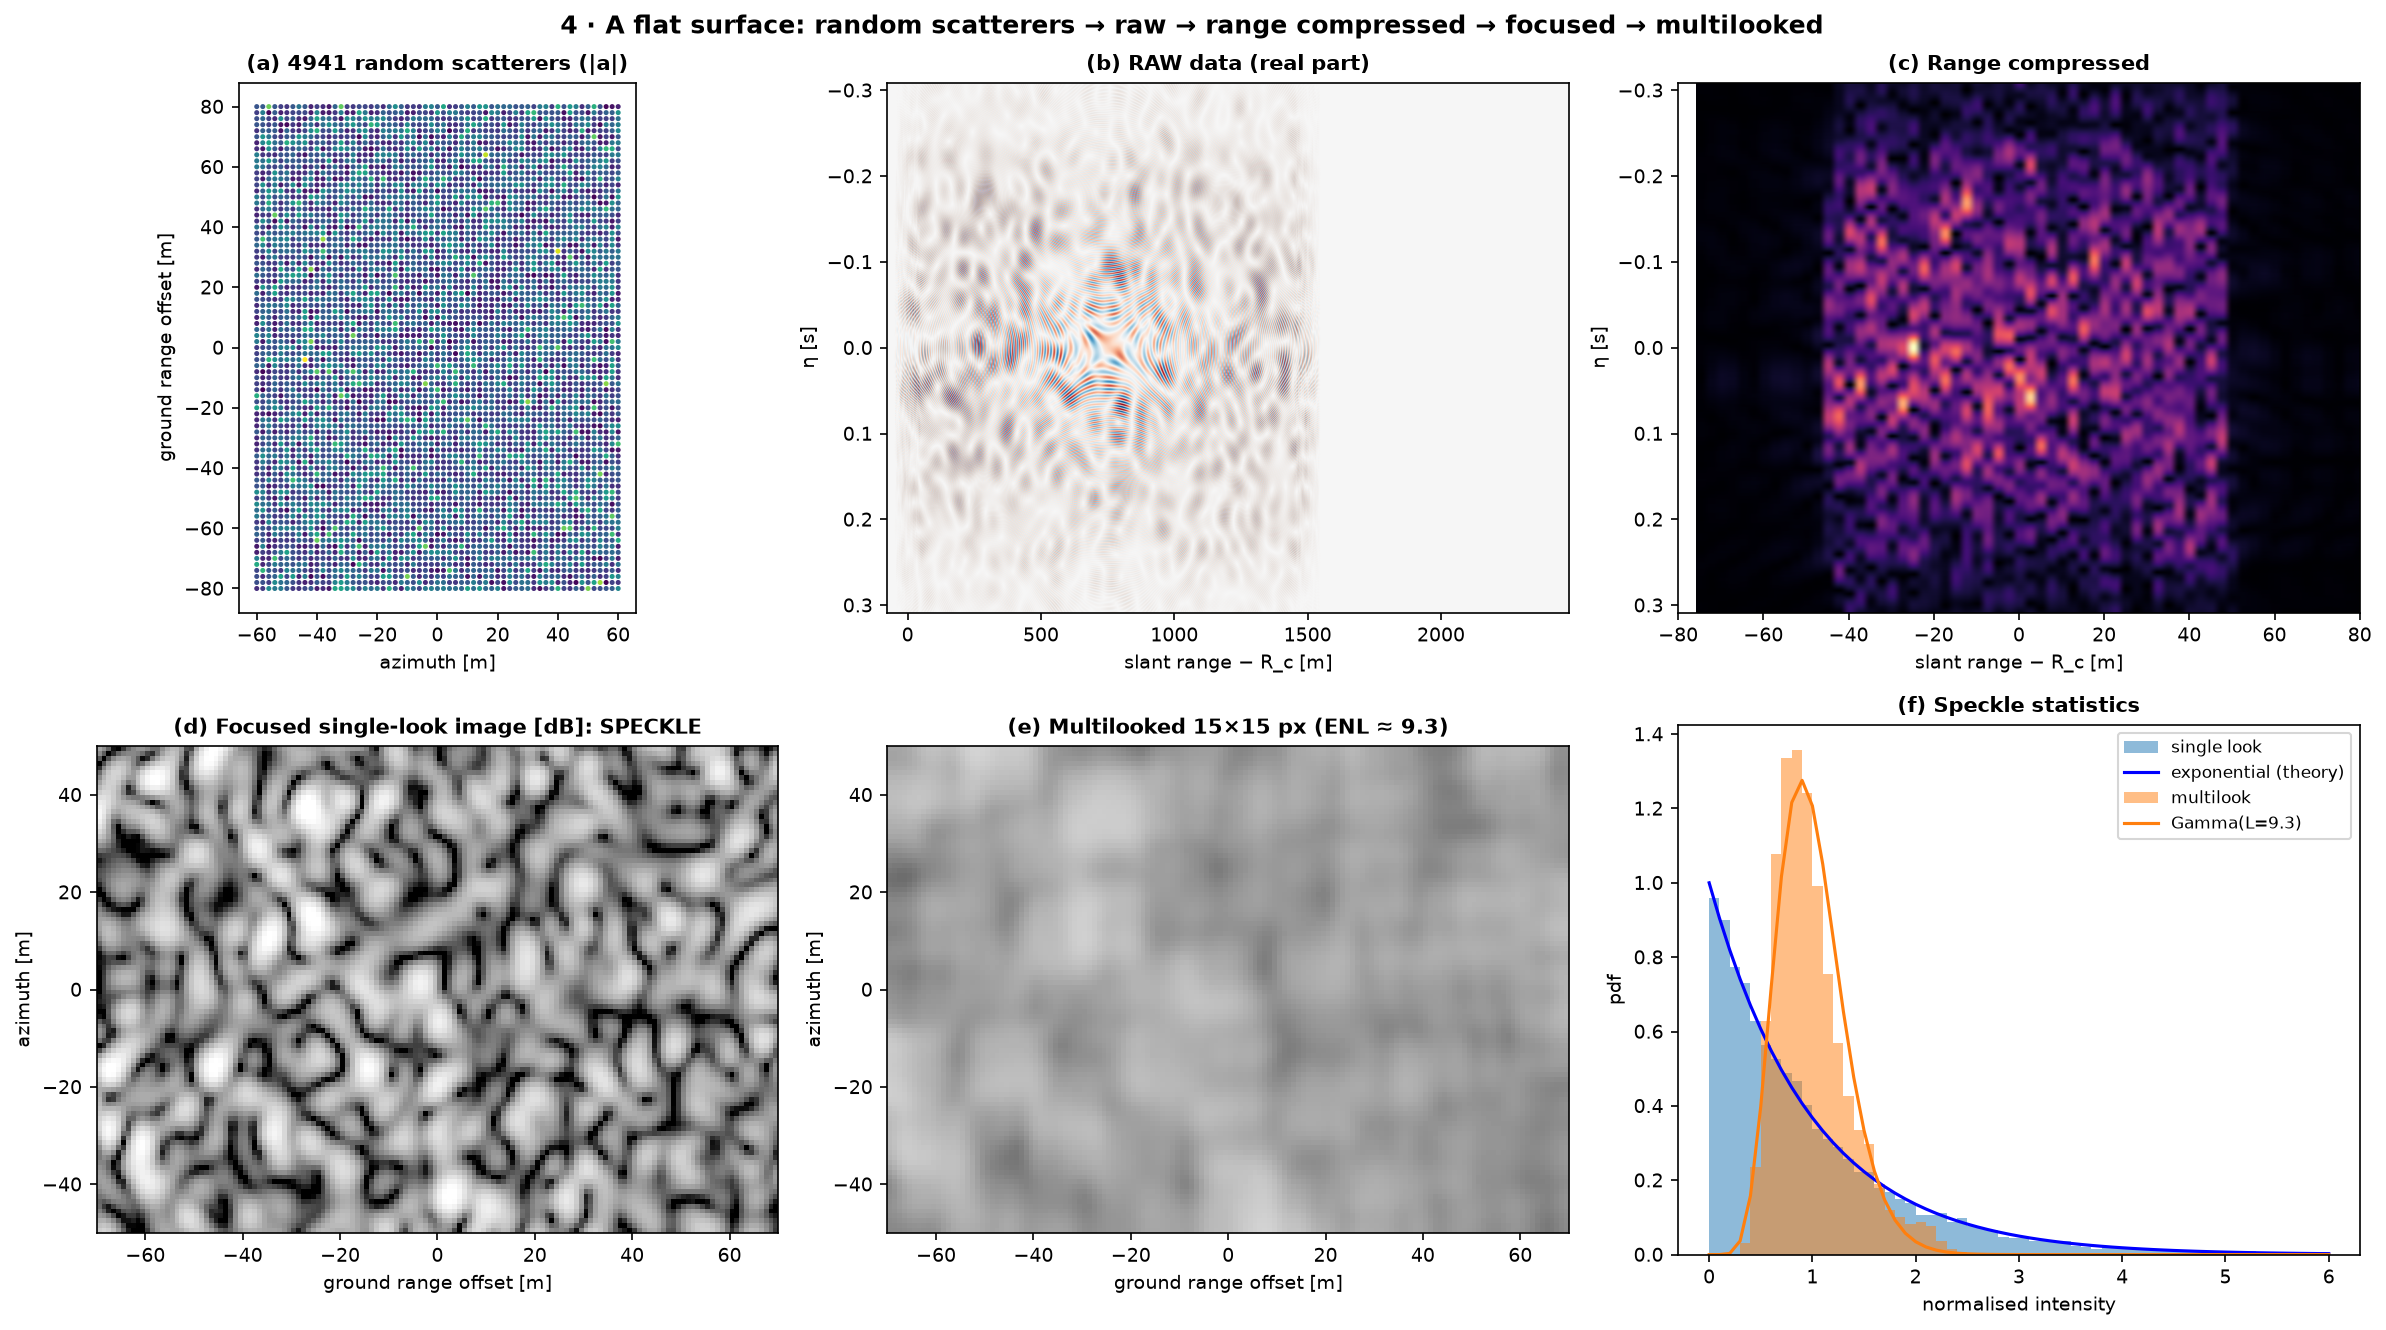
\includegraphics[width=\figw]{04_flat_surface_speckle.png}
\caption{Distributed scatterers: (\textbf{a}) random scatterer field; (\textbf{b}) raw data; (\textbf{c}) range-compressed data; (\textbf{d}) focused single-look image; (\textbf{e}) multilooked image; (\textbf{f}) intensity statistics compared with the exponential and Gamma distributions.}
\label{fig:flat}
\end{figure}
\begin{figure}[htbp]
\centering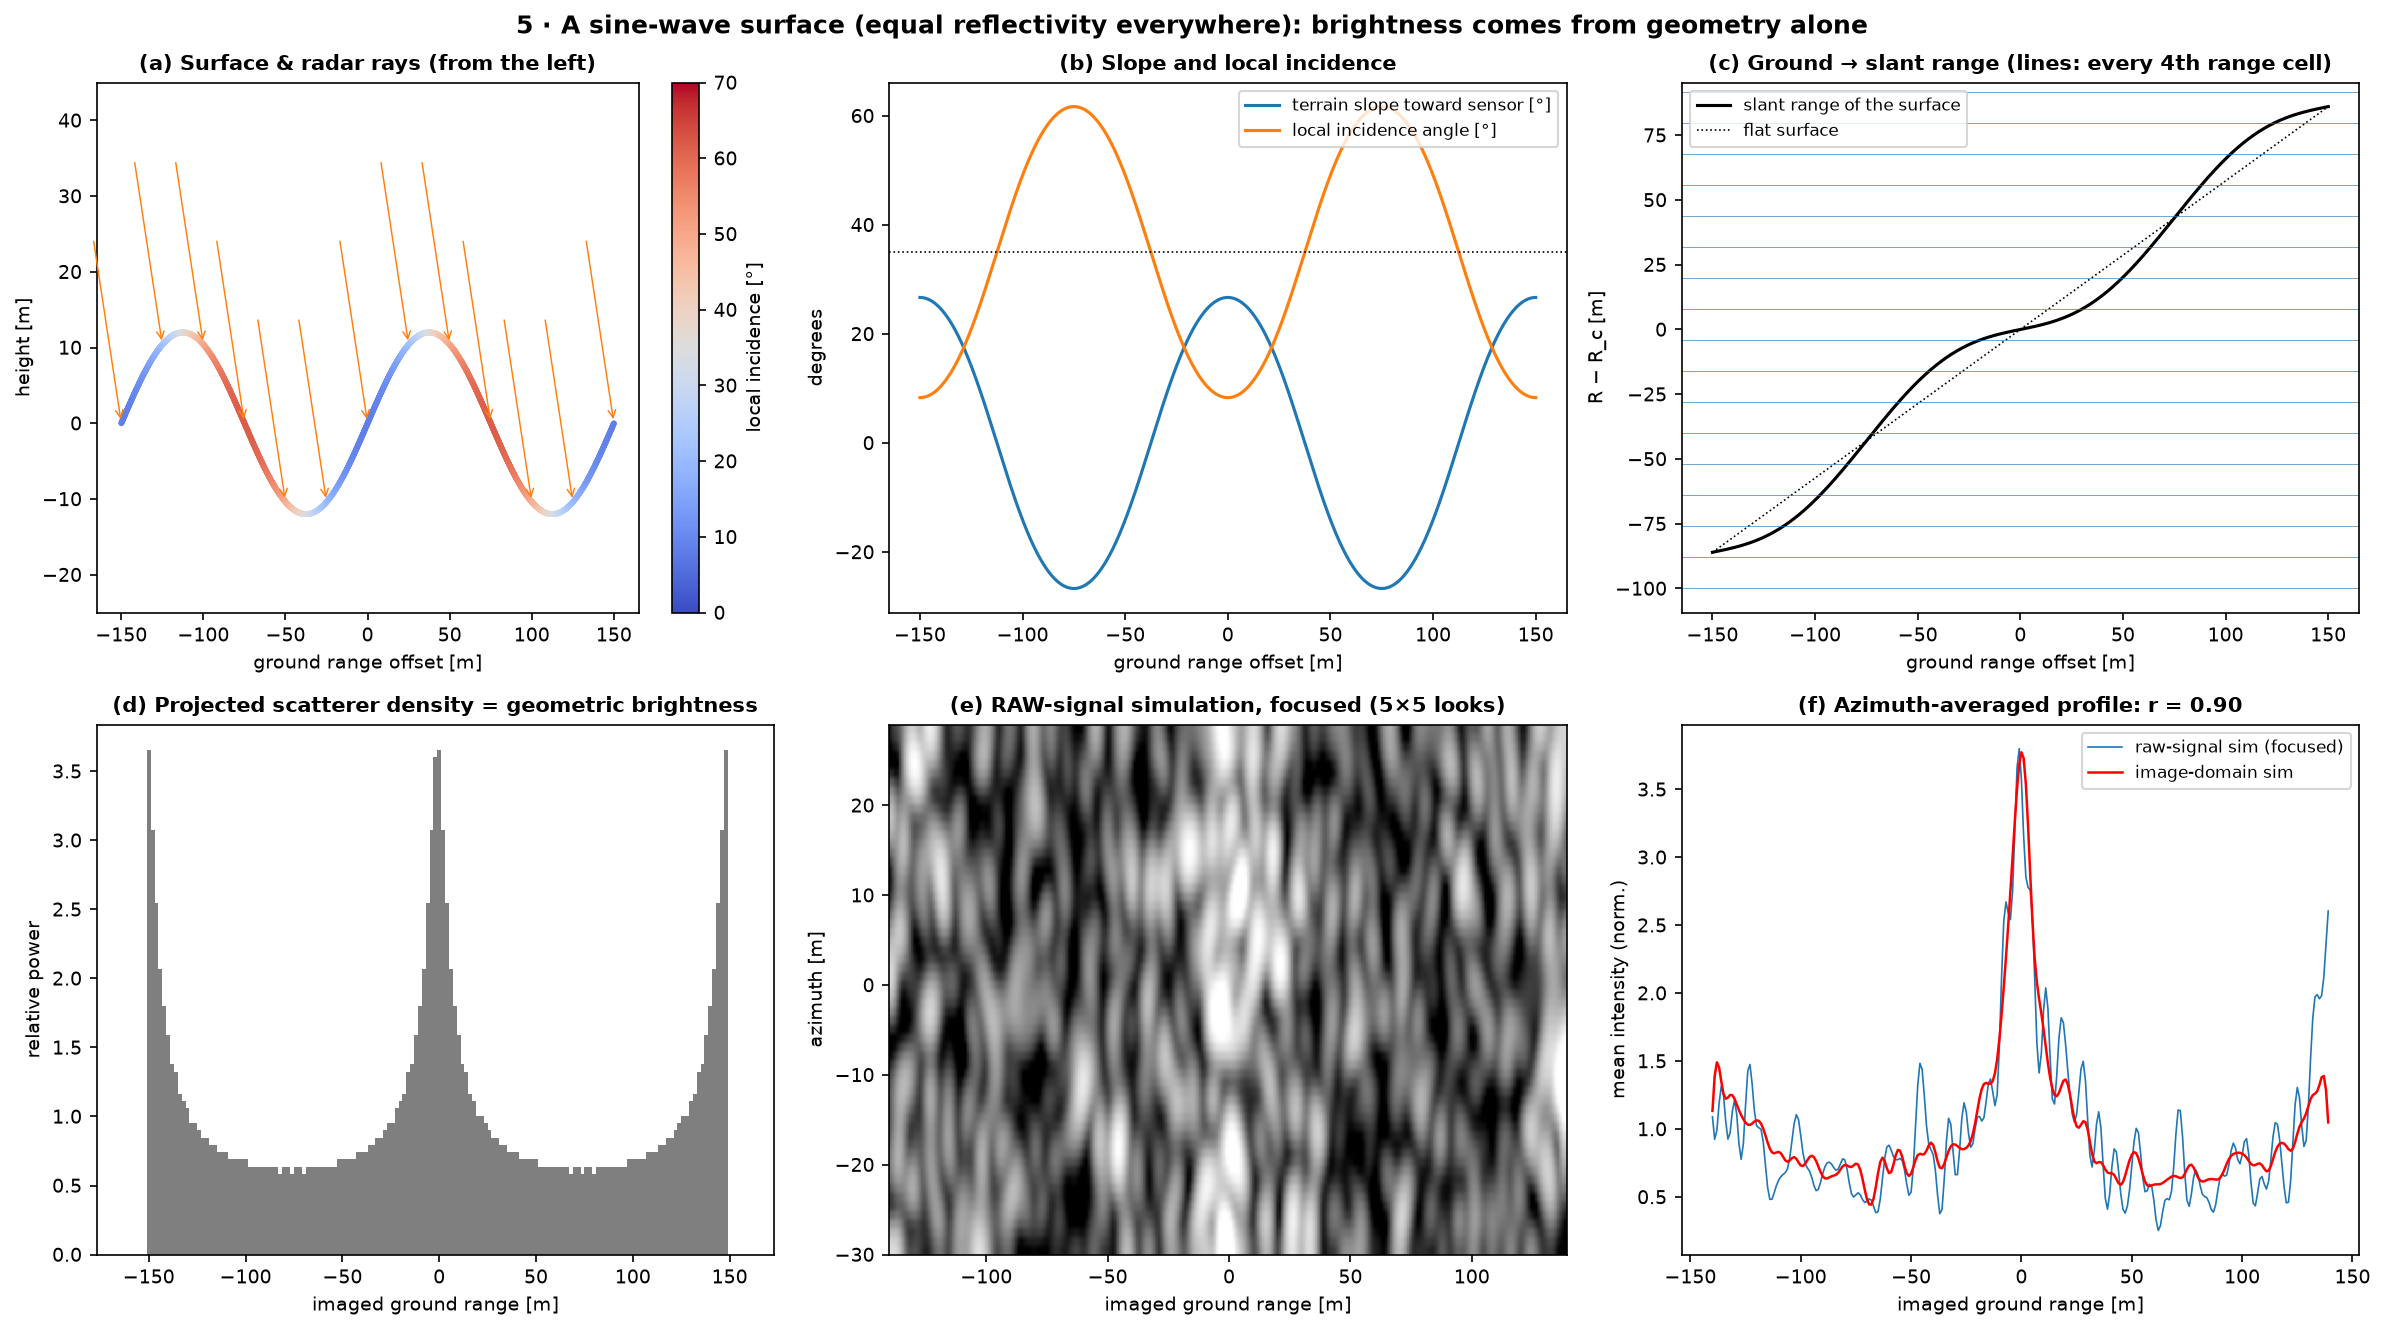
\includegraphics[width=\figw]{05_sine_surface.png}
\caption{Sinusoidal surface with uniform reflectivity: (\textbf{a}) profile and radar rays; (\textbf{b}) slope and local incidence angle; (\textbf{c}) ground-to-slant-range mapping; (\textbf{d}) projected scatterer density; (\textbf{e}) focused raw-signal simulation; (\textbf{f}) azimuth-averaged profiles of the raw-signal and image-domain simulations.}
\label{fig:sine}
\end{figure}
\begin{figure}[htbp]
\centering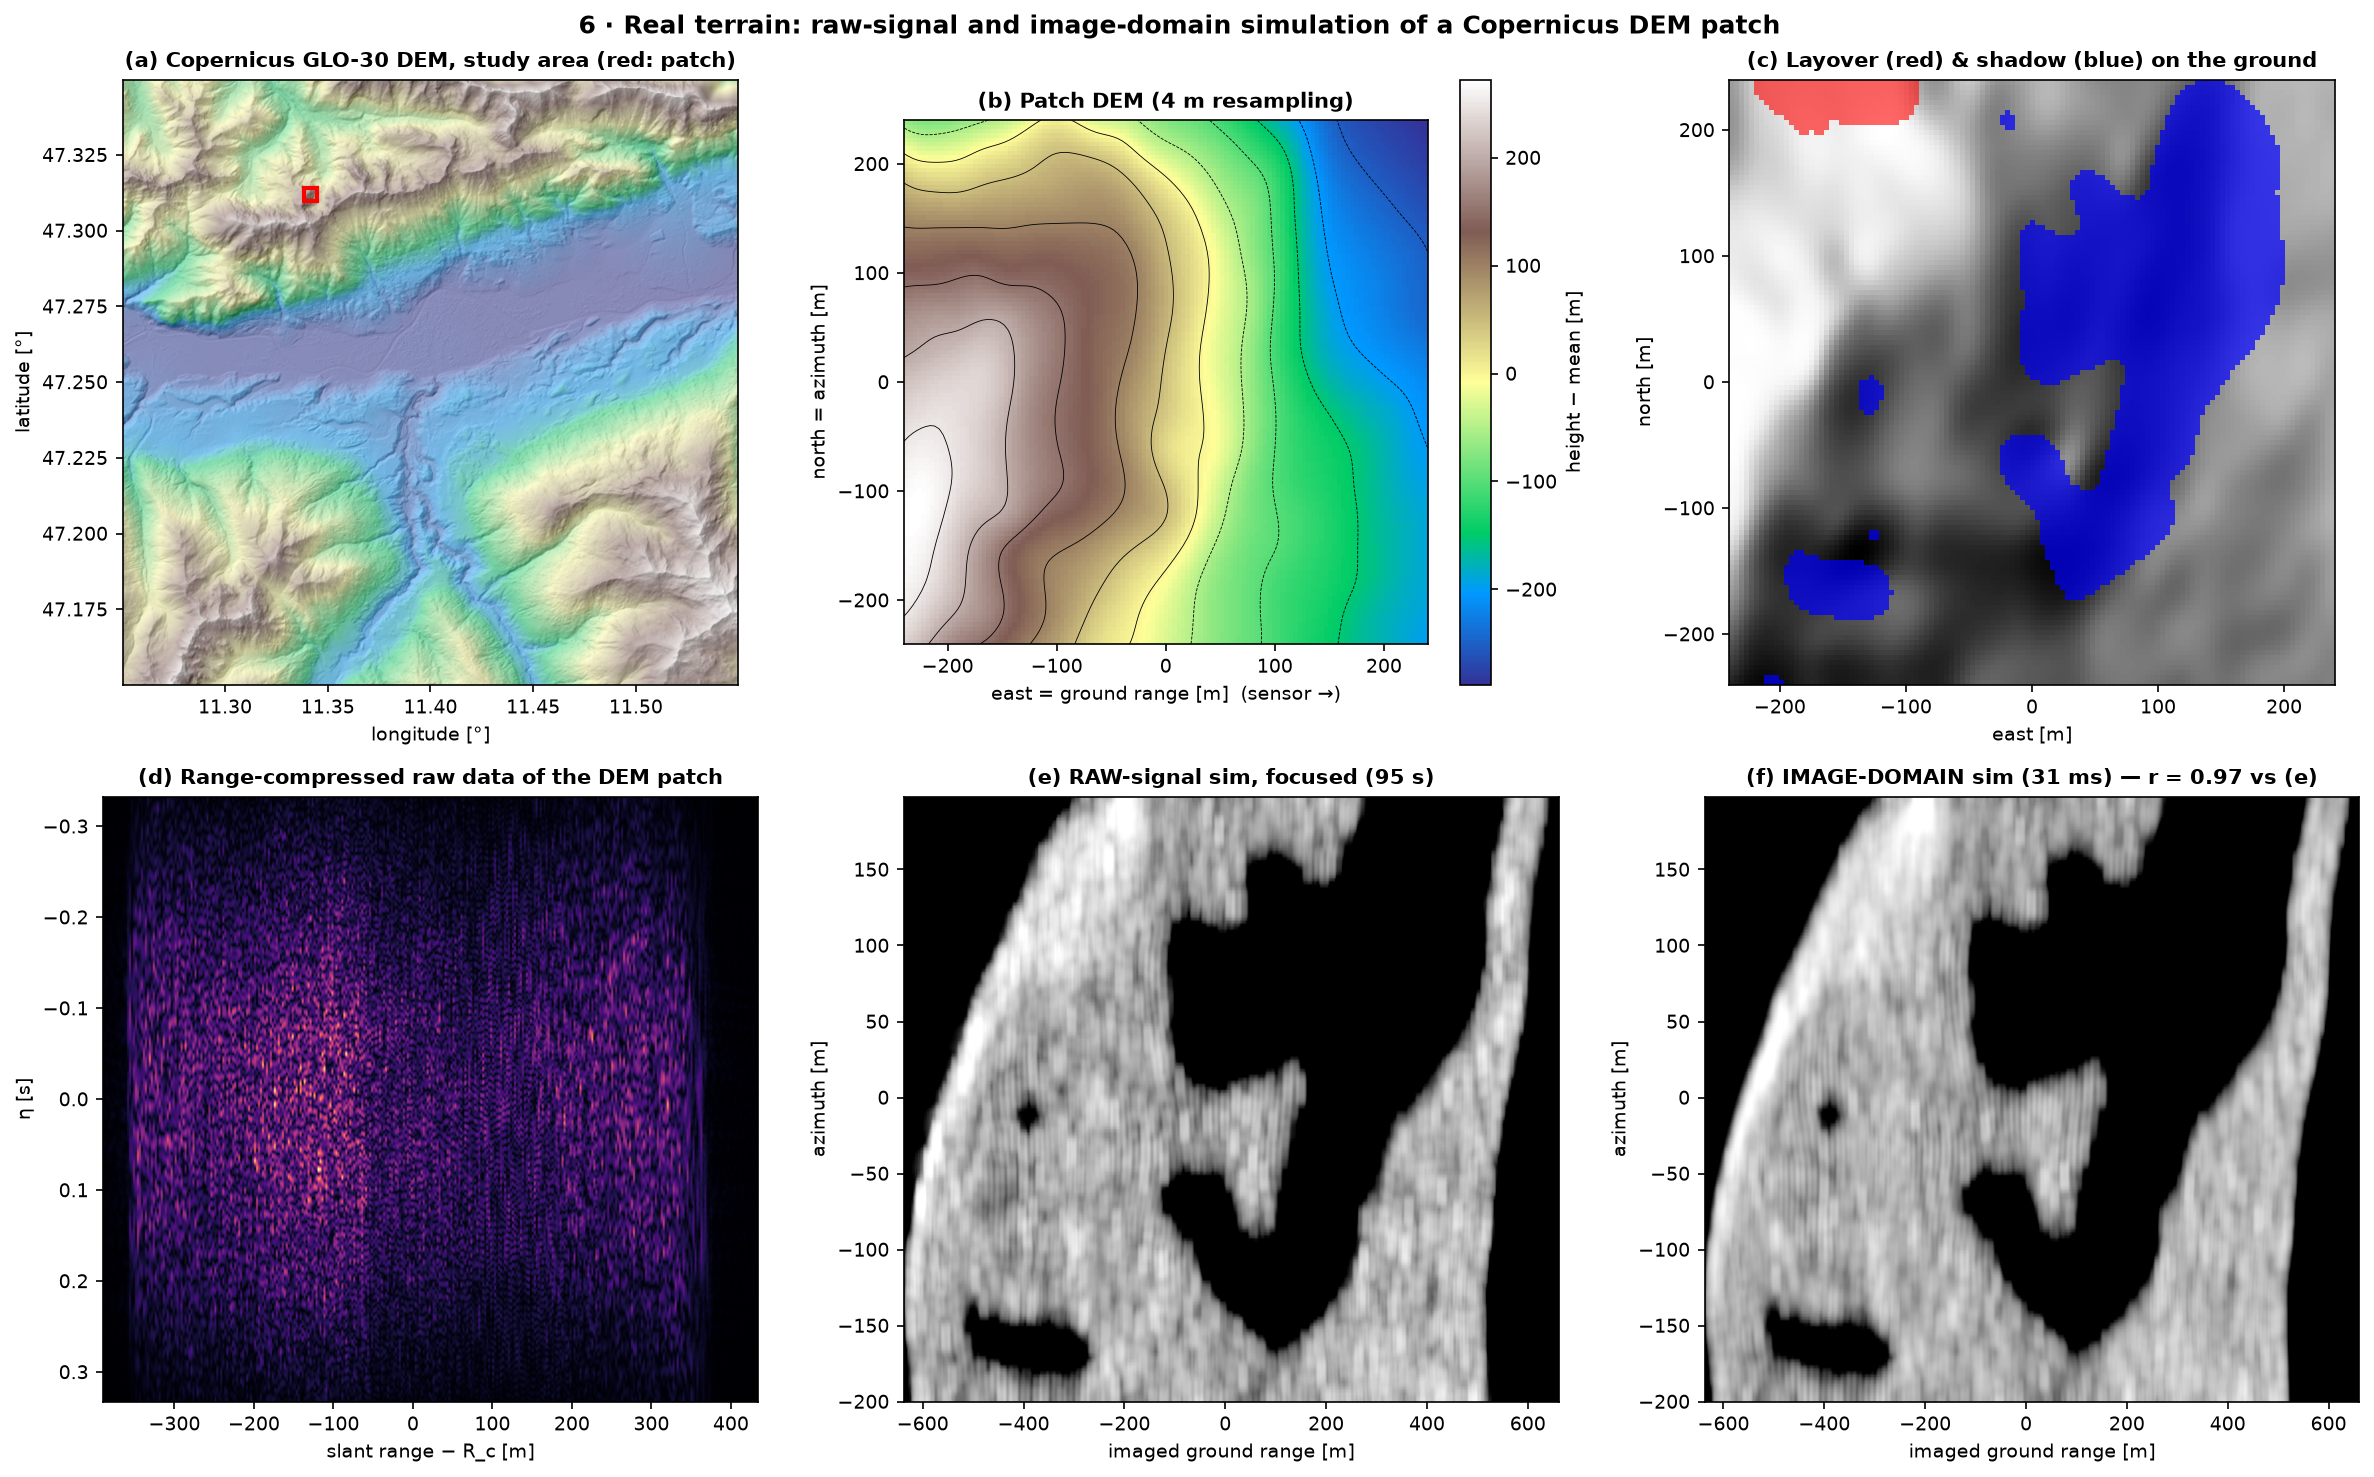
\includegraphics[width=\figw]{06_dem_patch_raw_vs_image_domain.png}
\caption{Copernicus DEM patch: (\textbf{a}) location; (\textbf{b}) patch DEM; (\textbf{c}) layover and shadow on the ground; (\textbf{d}) range-compressed raw data; (\textbf{e}) focused raw-signal simulation; (\textbf{f}) image-domain simulation.}
\label{fig:dempatch}
\end{figure}

\subsection{Geometric Distortions over the Study Site}
On a synthetic profile with a 55$^\circ$ fore-slope and a 65$^\circ$ back-slope observed at a 35$^\circ$ look angle, the shadow and layover criteria classify the fore-slope as active layover, the valley floor in front of it as passive layover, the back-slope and the plain behind it as shadow, and a gentle hill with a maximum slope of about 20$^\circ$ as foreshortened only (Figure~\ref{fig:geomprofile}). On a $9\times9$\,km subset of the study site, layover affects 18\,\% of the area at a look angle of 20$^\circ$ and decreases to about 1\,\% at 50$^\circ$, while shadow increases from 0 to 3.4\,\% (Figure~\ref{fig:geomdem}), which illustrates the classical trade-off in the choice of incidence angle over mountains~\cite{kropatsch1990,gelautz1998}. Figure~\ref{fig:radio} builds the simulated image in the order of the physics: local incidence angle, $\sigz(\theta_{loc})$, illuminated area, their product, speckle and multilooking. The geometric term alone, i.e., the illuminated area per pixel, already reproduces most of the image structure.

\begin{figure}[htbp]
\centering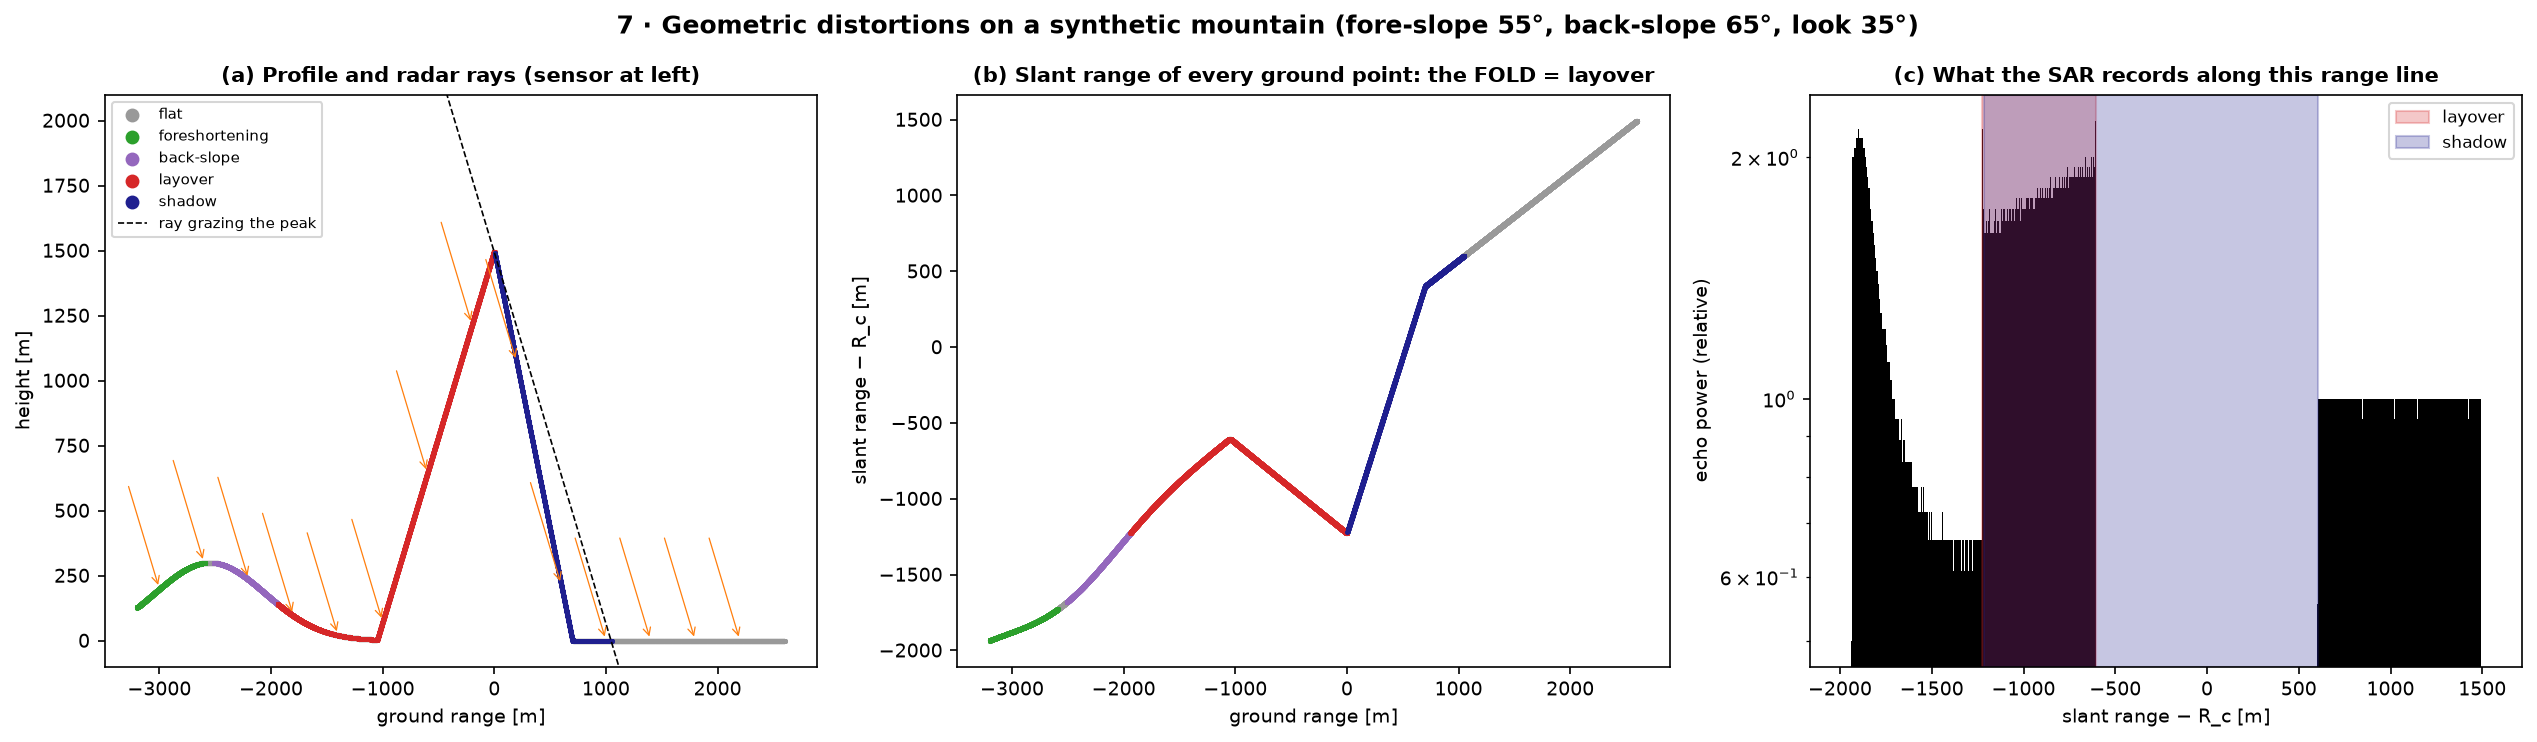
\includegraphics[width=\figw]{07_geometric_distortions_profile.png}
\caption{Geometric distortions along a synthetic profile: (\textbf{a}) classification and radar rays; (\textbf{b}) slant range of every ground point, where the fold indicates layover; (\textbf{c}) echo power recorded along the range line.}
\label{fig:geomprofile}
\end{figure}
\begin{figure}[htbp]
\centering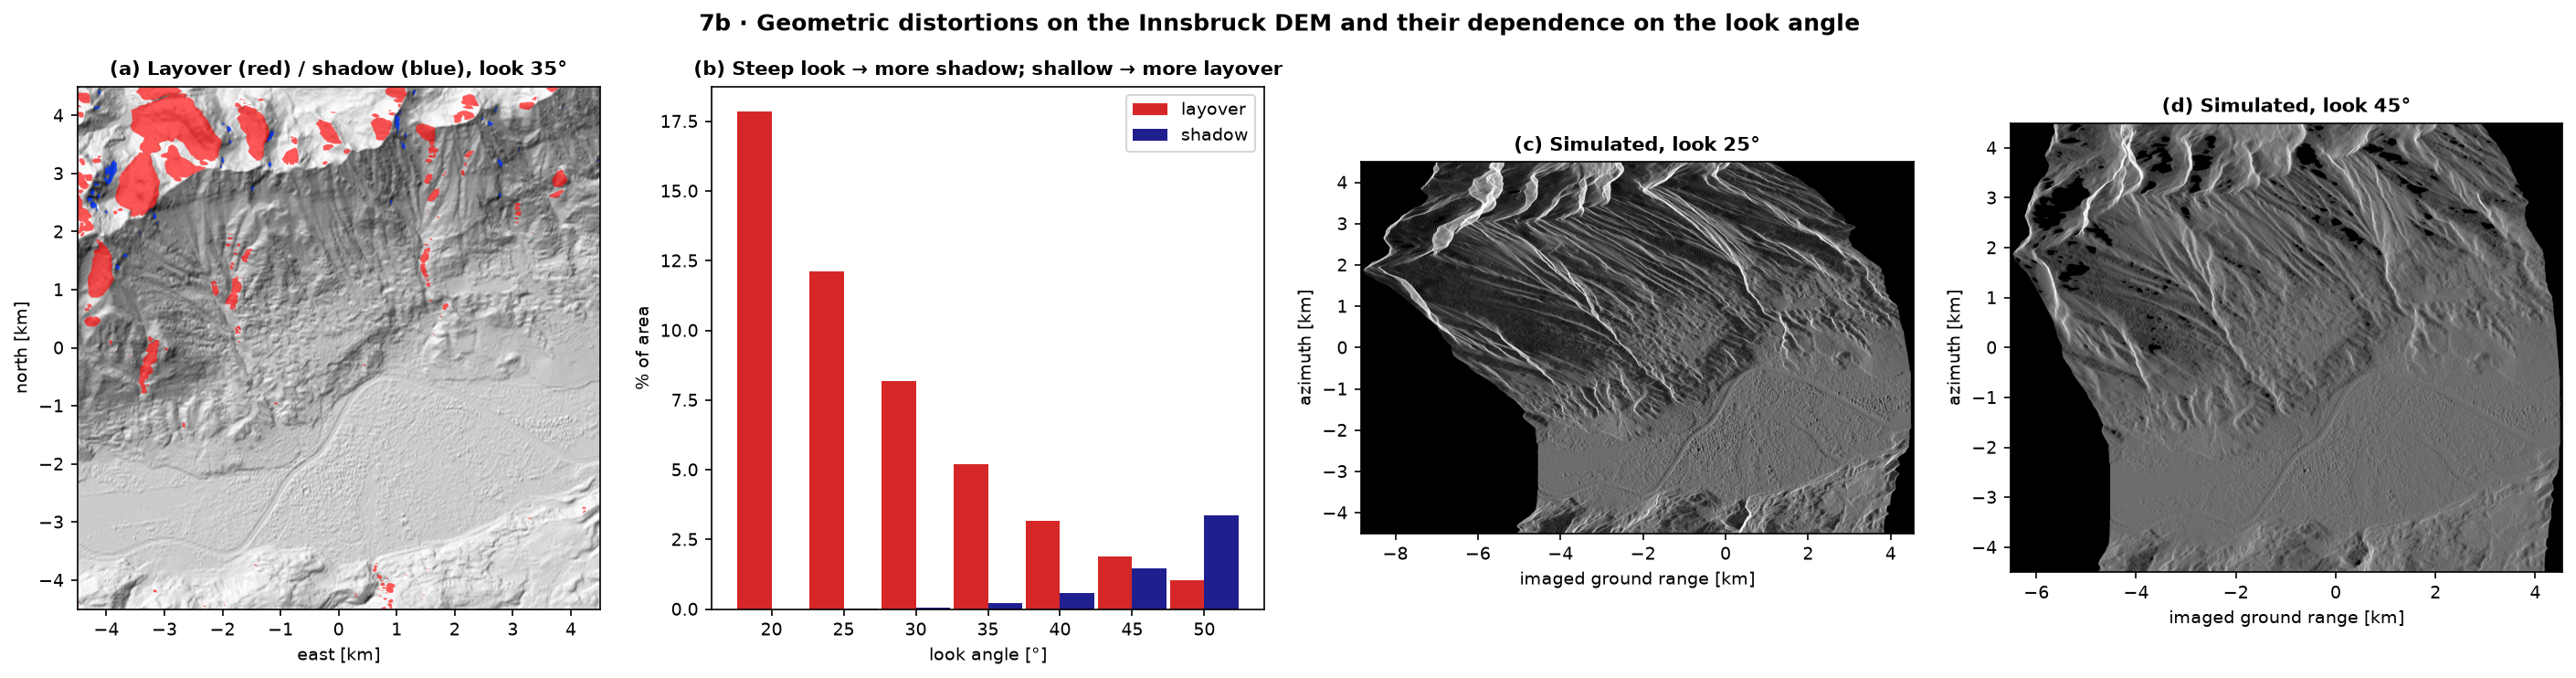
\includegraphics[width=\figw]{07b_geometric_distortions_dem.png}
\caption{Layover and shadow over a $9\times9$\,km subset of the study site (\textbf{a}), their fraction as a function of the look angle (\textbf{b}), and simulated images at look angles of 25$^\circ$ (\textbf{c}) and 45$^\circ$ (\textbf{d}).}
\label{fig:geomdem}
\end{figure}
\begin{figure}[htbp]
\centering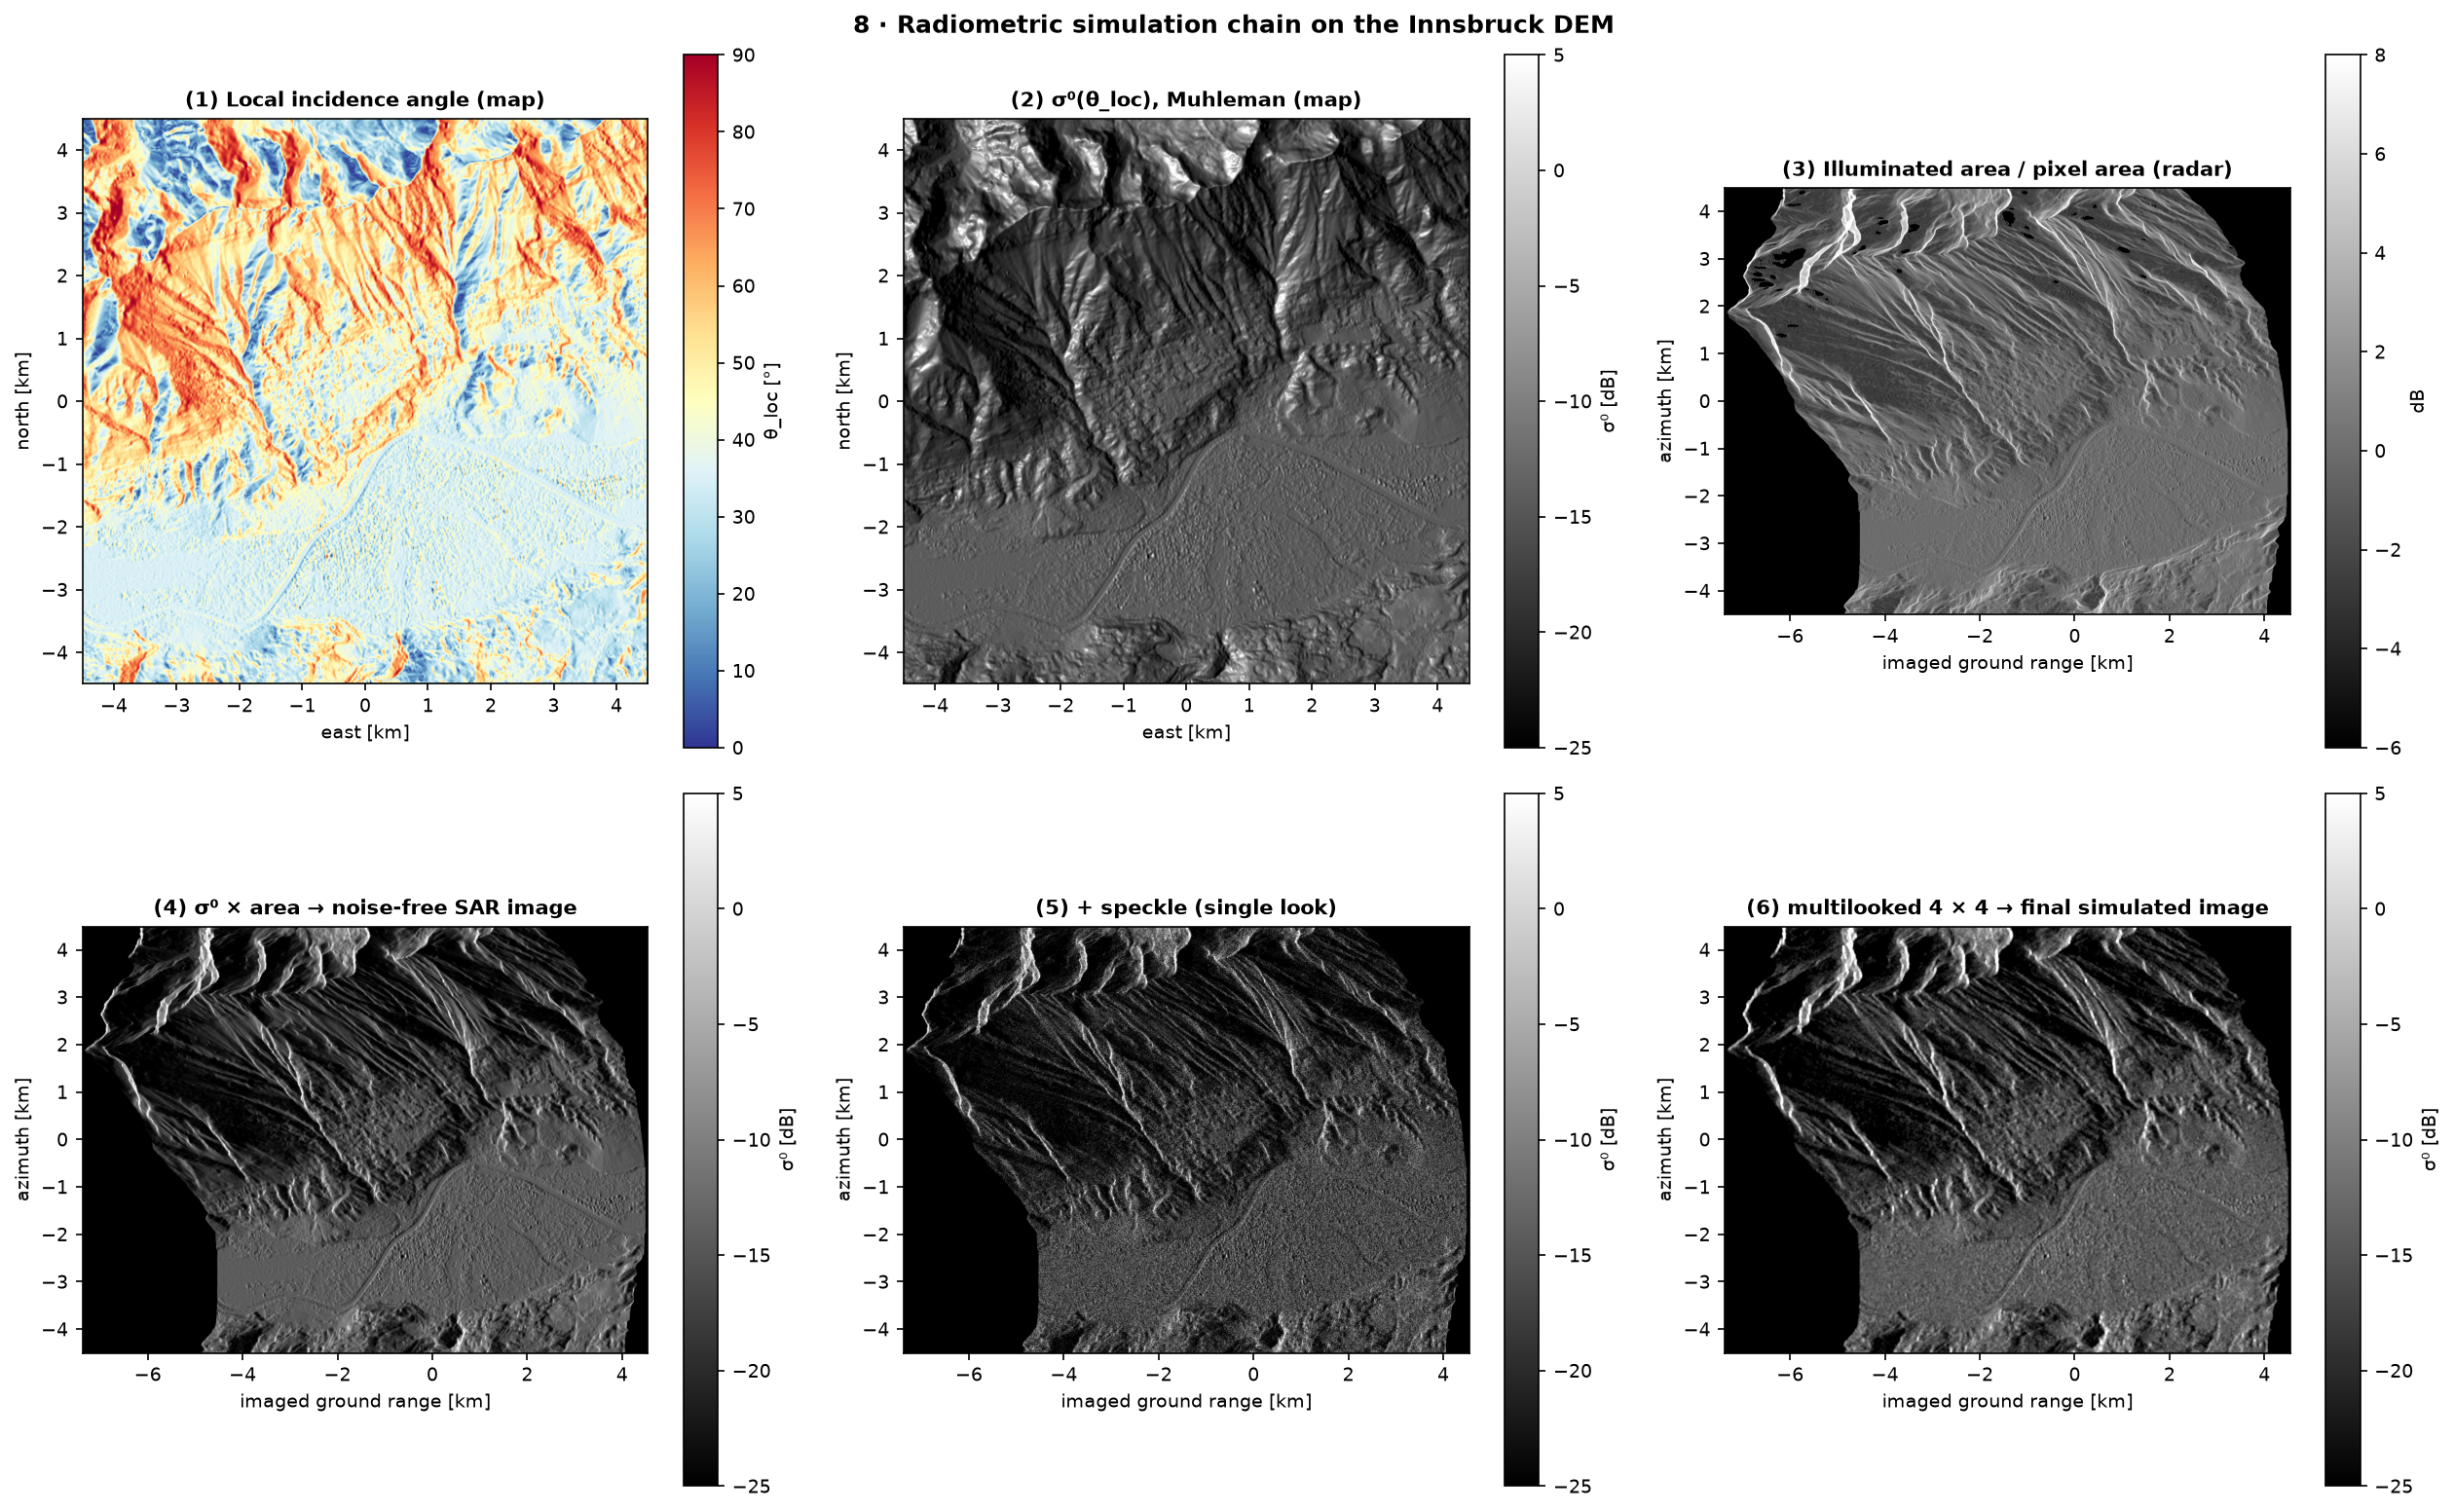
\includegraphics[width=\figw]{08b_radiometric_chain.png}
\caption{Radiometric simulation chain: (\textbf{1}) local incidence angle; (\textbf{2}) $\sigz$ from Muhleman's law in map geometry; (\textbf{3}) illuminated area per pixel in radar geometry; (\textbf{4}) noise-free simulated image; (\textbf{5}) single-look speckle; (\textbf{6}) multilooked image.}
\label{fig:radio}
\end{figure}

\subsection{Geocoding Accuracy}
\label{sec:res-geo}
With the valid-from rule for the SRGR polynomials, the range-Doppler geocoding reproduces the geolocation grid of both products to \geoDpixMax{} pixels in range, \geoDtMax{} ms in zero-Doppler time (\geoDlineMax{} lines) and \geoDRmax{} mm in slant range over all \nGrid{} tie points of each scene (Figure~\ref{fig:geomval}a). Linear interpolation between the polynomial sets increased the maximum range error to 3.3 pixels (Figure~\ref{fig:design}, iteration 5). The line numbers tabulated in the geolocation grid are nominal and deviate by up to 0.2 lines from the zero-Doppler times listed for the same points; the latter must be used for validation.

\subsection{Comparison with Sentinel-1 and Choice of the Backscatter Law}
Figure~\ref{fig:realsim} compares the real ascending image with the simulation. Ridges, valleys, bright fore-slopes, layover bands and black shadows of the real image are reproduced at the right positions, while the urbanised valley floor appears as a uniform surface in the simulation. Table~\ref{tab:models} and Figure~\ref{fig:models} summarise the agreement for the five backscatter laws. The constant law, which only contains the illuminated-area term, already reaches $r=0.53$. Laws that decrease with $\theta_{loc}$ improve the agreement substantially, but no single law is best for every metric: Muhleman's law gives the highest correlation ($r=\rMuAsc$), the Lambert and fitted laws the highest SSIM, and the cosine law the lowest RMSE. The fitted law has an exponent $n=\nFit$ and $10\log_{10}k=\kFitDb$\,dB, i.e., the data select Lambert's law (Figure~\ref{fig:fit}). It describes the median real $\sigz$ well between 10$^\circ$ and 80$^\circ$, whereas at small local incidence angles the real backscatter rises more steeply, which Muhleman's law captures; these few very bright pixels weigh heavily in the Pearson correlation. The interquartile range of the real $\sigz$ at a given $\theta_{loc}$ is about 5\,dB, which indicates that land cover, rather than the angular law, limits the agreement.

\begin{figure}[htbp]
\centering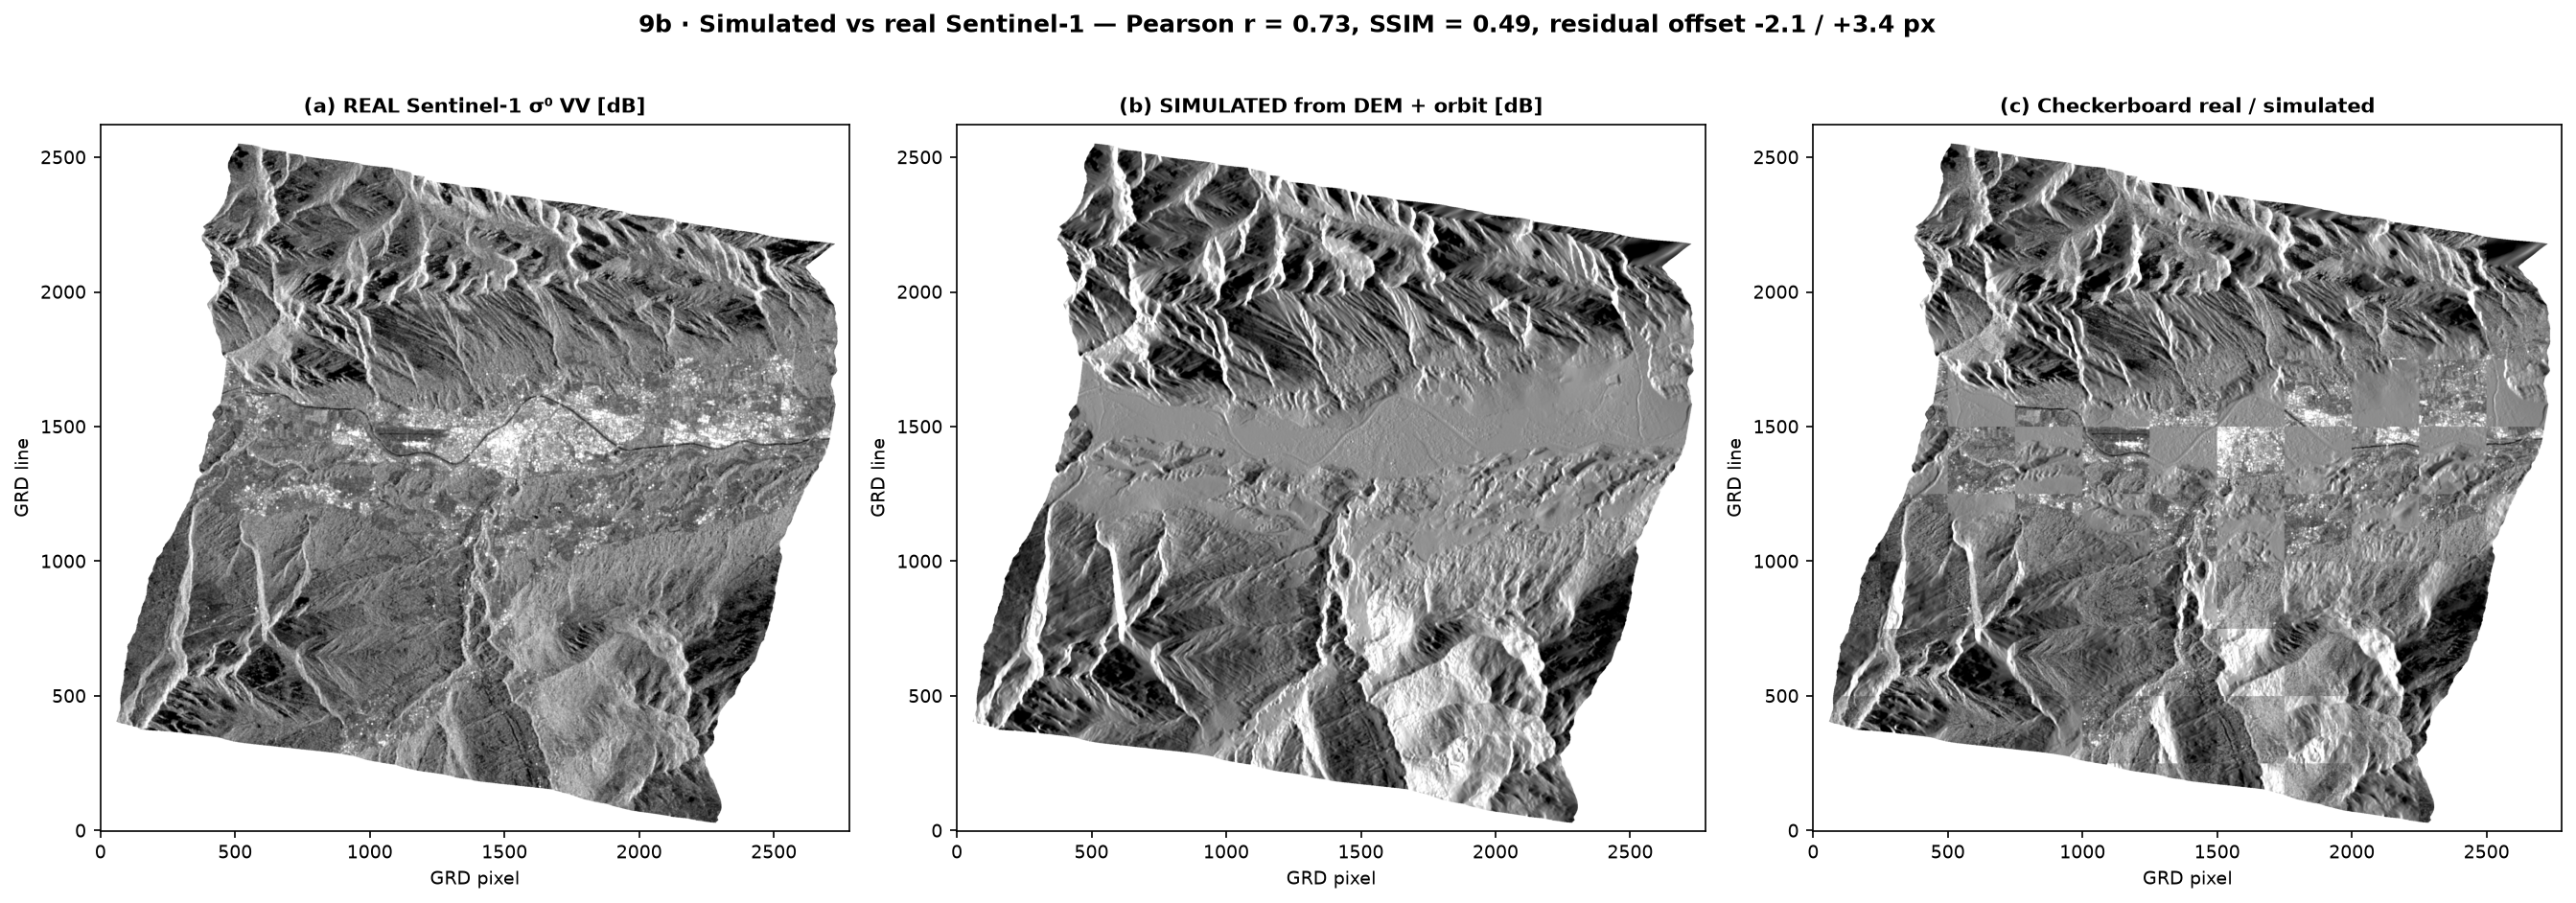
\includegraphics[width=\figw]{09b_real_vs_simulated.png}
\caption{Real Sentinel-1 $\sigz$ (\textbf{a}), simulation with Muhleman's law (\textbf{b}) and a checkerboard of both (\textbf{c}); ascending scene, radar geometry.}
\label{fig:realsim}
\end{figure}

\begin{table}[htbp]
\caption{Agreement between the real and the simulated ascending image for five backscatter laws ($5\times5$ multilook, dB). The level offset is the constant added to the law to calibrate its absolute level.}
\label{tab:models}
\centering\small
\begin{tabular}{lrrrrr}\toprule
 Backscatter model & Pearson $r$ & Spearman $\rho$ & SSIM & RMSE [dB] & level offset [dB]\\\midrule
Constant & 0.534 & 0.739 & 0.377 & 3.83 & -0.6 \\
$\cos\theta_{loc}$ & 0.663 & 0.767 & 0.467 & 3.72 & -8.3 \\
$\cos^2\theta_{loc}$ (Lambert) & 0.703 & 0.762 & 0.509 & 4.44 & -6.1 \\
Muhleman & 0.734 & 0.757 & 0.494 & 4.58 & 7.6 \\
Fitted $k\cos^{1.98}\theta_{loc}$ & 0.710 & 0.761 & 0.508 & 4.29 & -1.4 \\
\bottomrule\end{tabular}

\end{table}

\begin{figure}[htbp]
\centering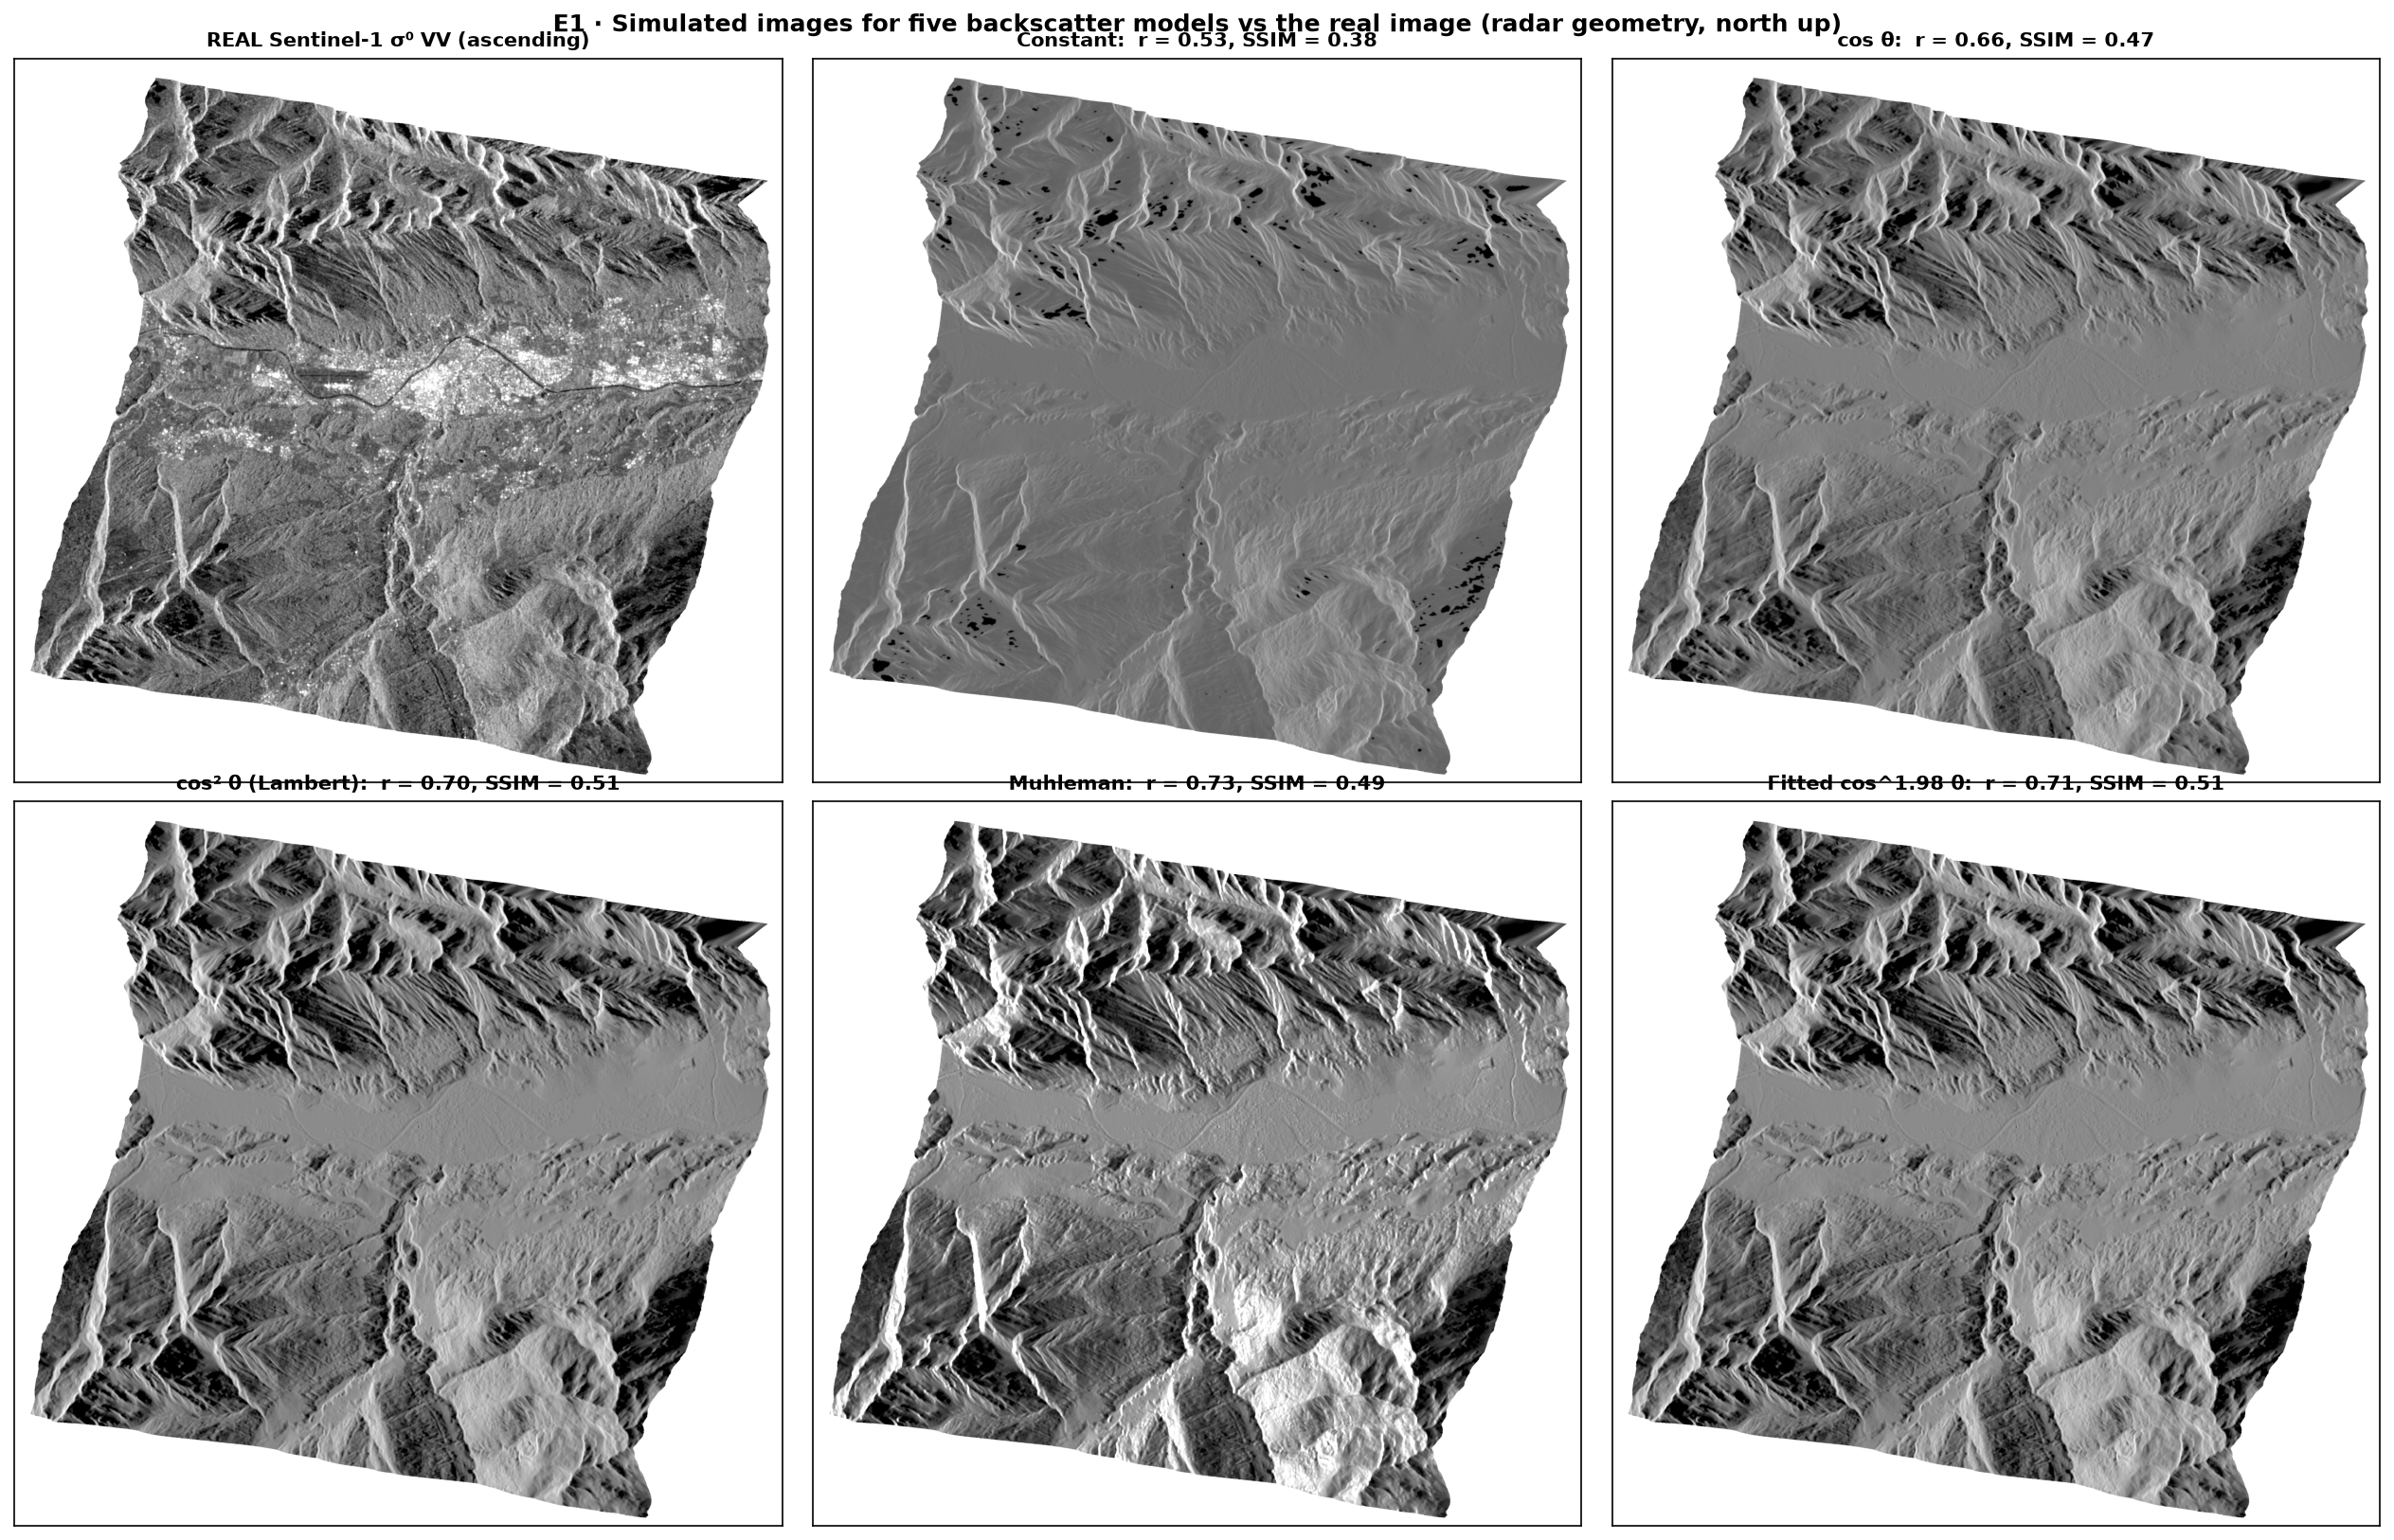
\includegraphics[width=\figw]{p1_models_images.png}
\caption{Real ascending image and simulations with the five backscatter laws (radar geometry, north up).}
\label{fig:models}
\end{figure}
\begin{figure}[htbp]
\centering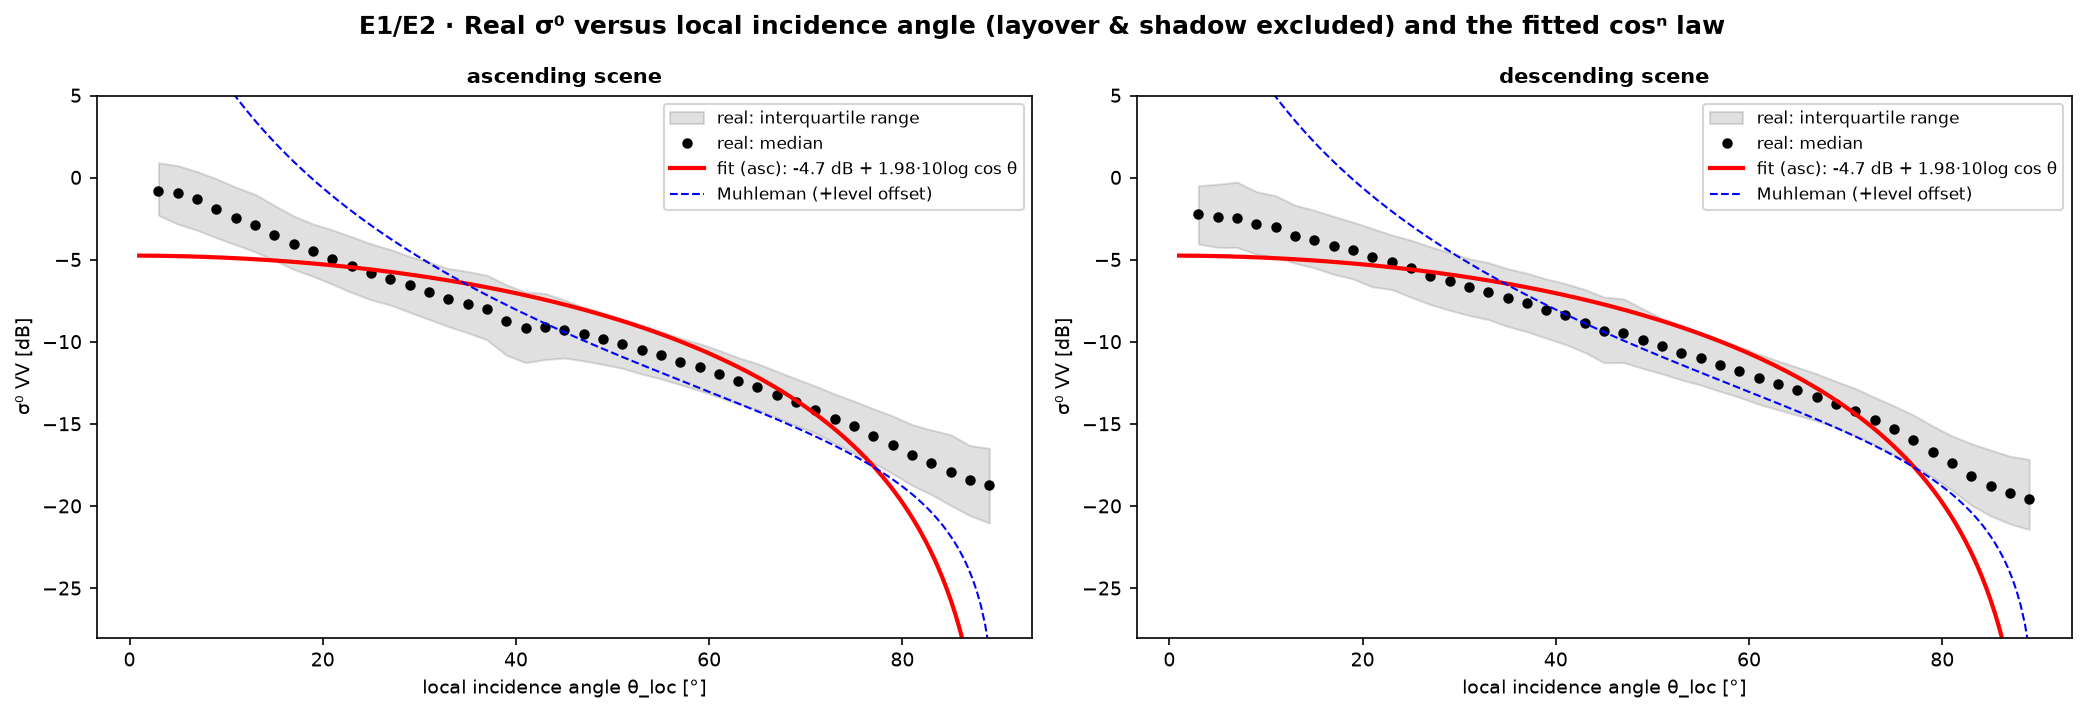
\includegraphics[width=\figw]{p2_fitted_model.png}
\caption{Real $\sigz$ as a function of the local incidence angle for the ascending (\textbf{a}) and descending (\textbf{b}) scenes, excluding layover and shadow, with the $\cos^n$ law fitted on the ascending scene and Muhleman's law.}
\label{fig:fit}
\end{figure}

\subsection{Second Viewing Geometry}
The descending scene looks west, so that layover and shadow move to the opposite slopes (Figure~\ref{fig:ascdesc}). Applying the law fitted on the ascending scene without any change yields $r=\rDesc$, $\rho=\rhoDesc$, SSIM\,$=\ssimDesc$ and RMSE\,$=\rmseDesc$\,dB, compared with $r=\rAsc$, $\rho=\rhoAsc$, SSIM\,$=\ssimAsc$ and RMSE\,$=\rmseAsc$\,dB on the ascending scene (Figure~\ref{fig:scatter}). A refit on the descending scene gives $n=\nRefitDesc$. The empirical law therefore transfers between the two viewing geometries; it describes the terrain rather than the acquisition.

\begin{figure}[htbp]
\centering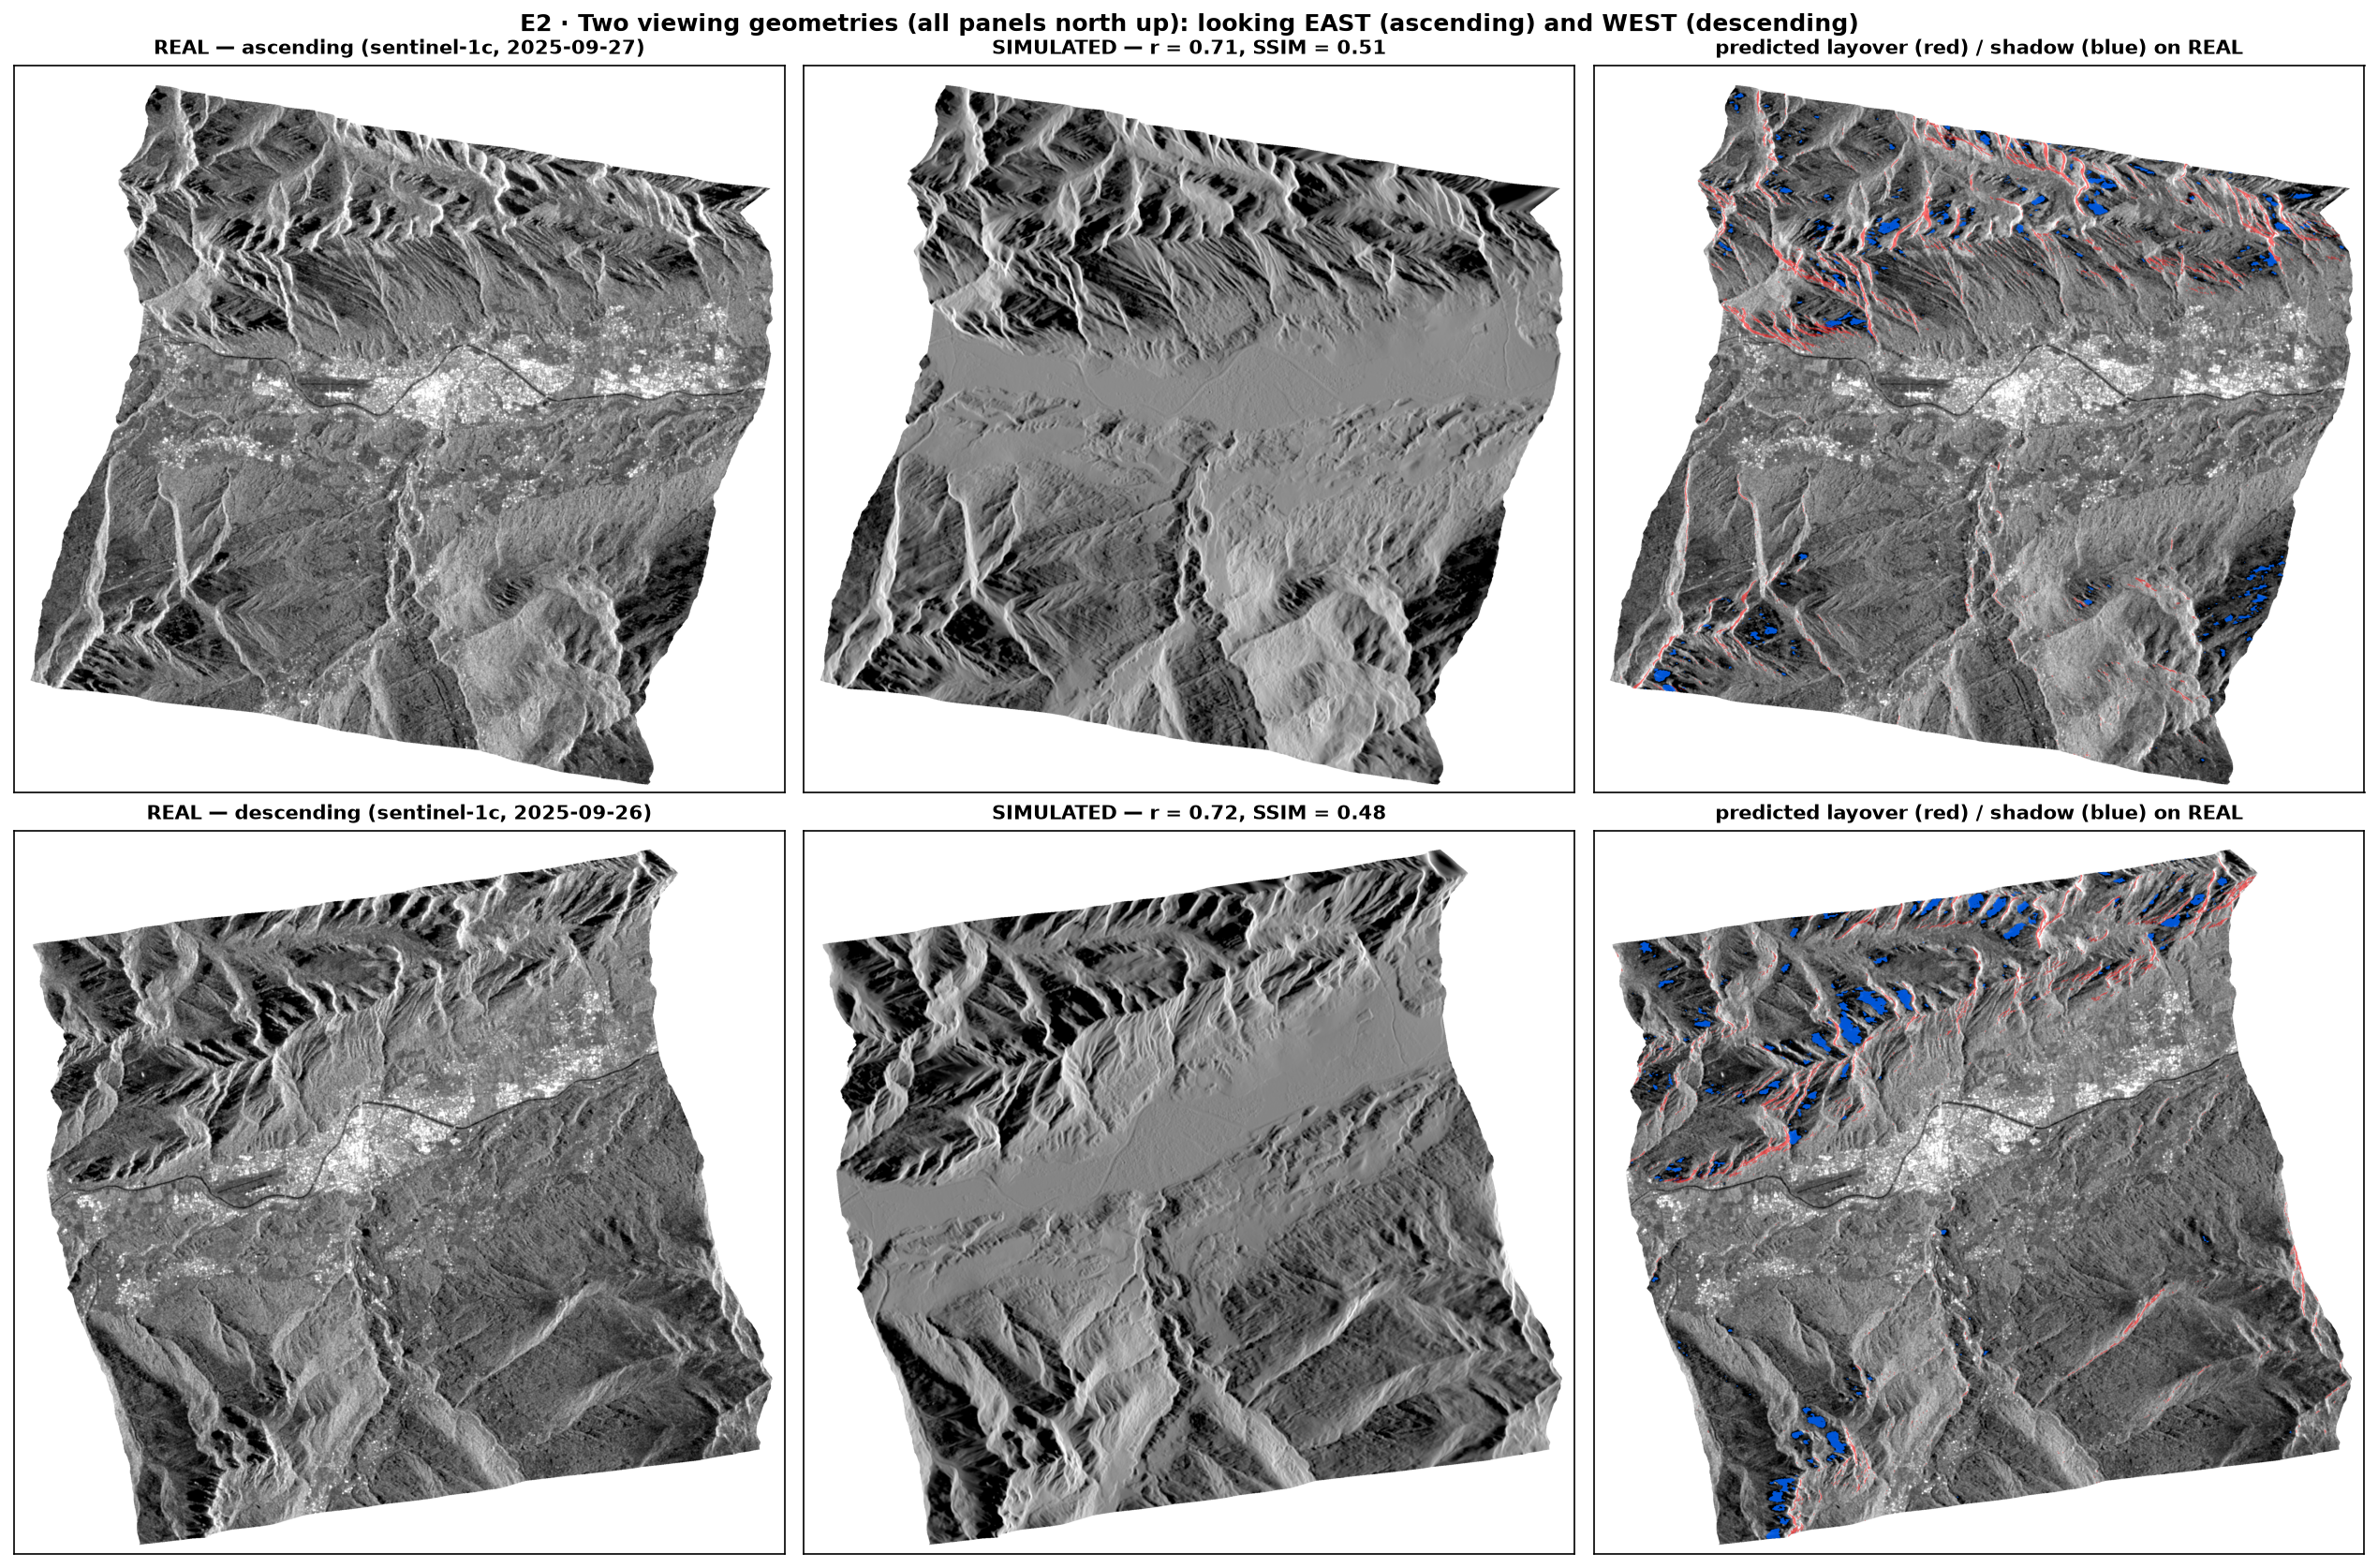
\includegraphics[width=\figw]{p3_ascending_descending.png}
\caption{Real and simulated images, and predicted layover (red) and shadow (blue) drawn on the real image, for the ascending (top, looking east) and descending (bottom, looking west) scenes; all panels north up.}
\label{fig:ascdesc}
\end{figure}
\begin{figure}[htbp]
\centering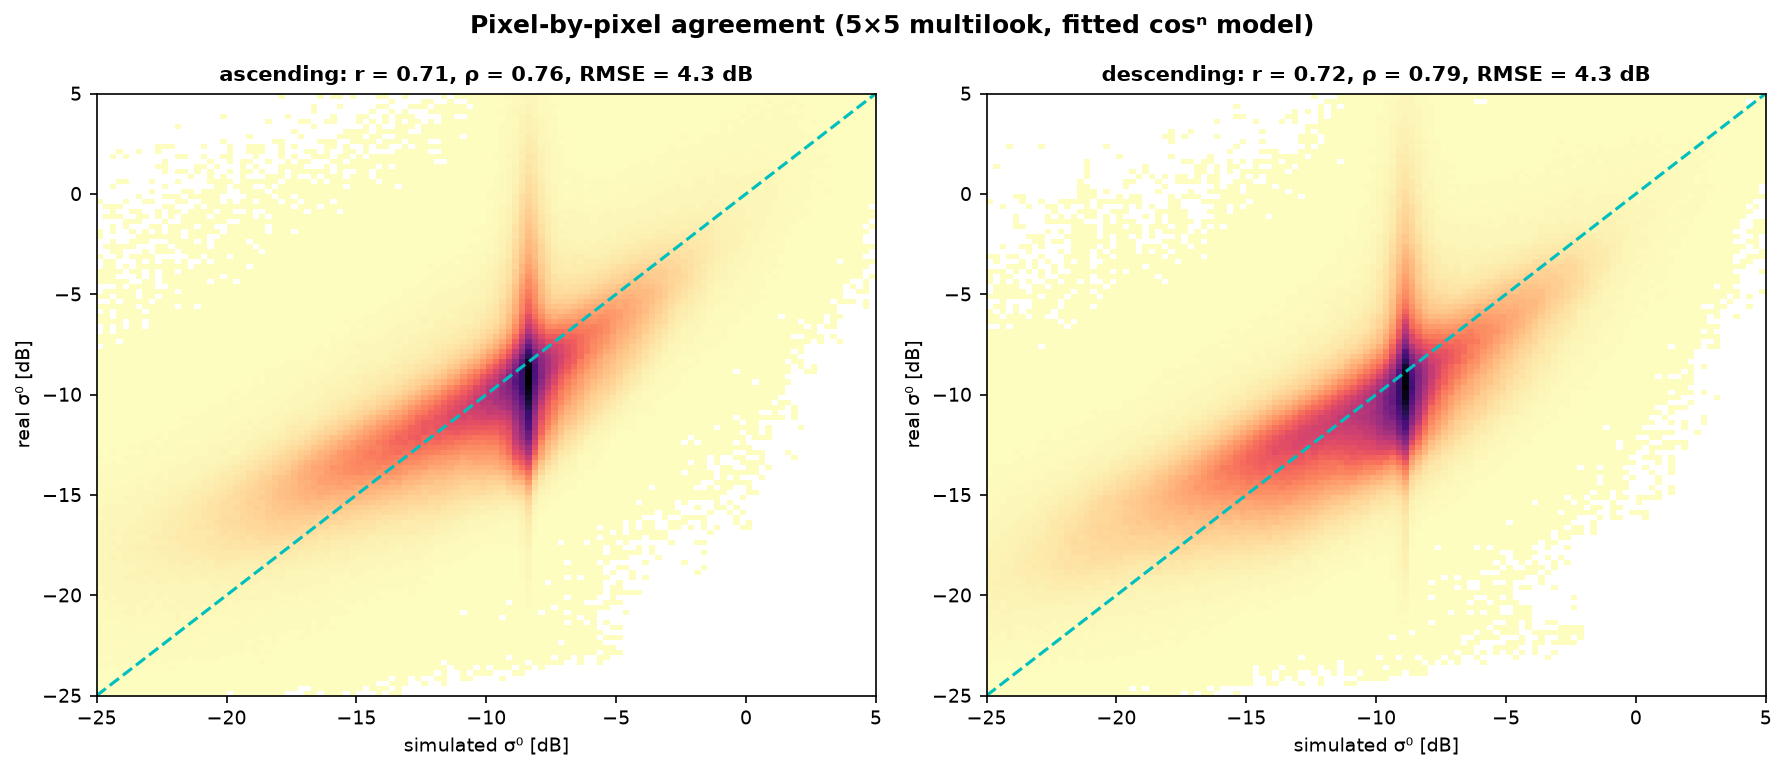
\includegraphics[width=0.86\textwidth]{p8_scatter.png}
\caption{Pixel-by-pixel comparison of real and simulated $\sigz$ for both scenes with the fitted law.}
\label{fig:scatter}
\end{figure}

\subsection{Validation of the Predicted Distortion Classes}
Table~\ref{tab:classes} and Figure~\ref{fig:geomval} test the predicted distortion classes against the real images. Pixels predicted to be in shadow are the darkest, with a median of $-21.0$\,dB (ascending) and $-22.0$\,dB (descending), i.e., at the noise floor of the sensor, since thermal noise was not removed. Pixels predicted to be in layover ($-3.5$ and $-3.9$\,dB) or strongly foreshortened ($-4.5$ and $-5.1$\,dB) are the brightest, about 7\,dB above the remaining terrain. The ordering of the classes is identical in both geometries.

\begin{table}[htbp]
\caption{Real $\sigz$ inside the distortion classes predicted by the simulation.}
\label{tab:classes}
\centering\small
\begin{tabular}{lrrrr}\toprule
 & \multicolumn{2}{c}{ascending} & \multicolumn{2}{c}{descending}\\
Predicted class & pixels & median $\sigma^0$ [dB] & pixels & median $\sigma^0$ [dB]\\\midrule
shadow & 47k & -21.0 & 66k & -22.0 \\
layover & 82k & -3.5 & 61k & -3.9 \\
foreshortened (area > 2x) & 228k & -4.5 & 220k & -5.1 \\
other terrain & 4525k & -10.8 & 4576k & -11.5 \\
\bottomrule\end{tabular}

\end{table}
\begin{figure}[htbp]
\centering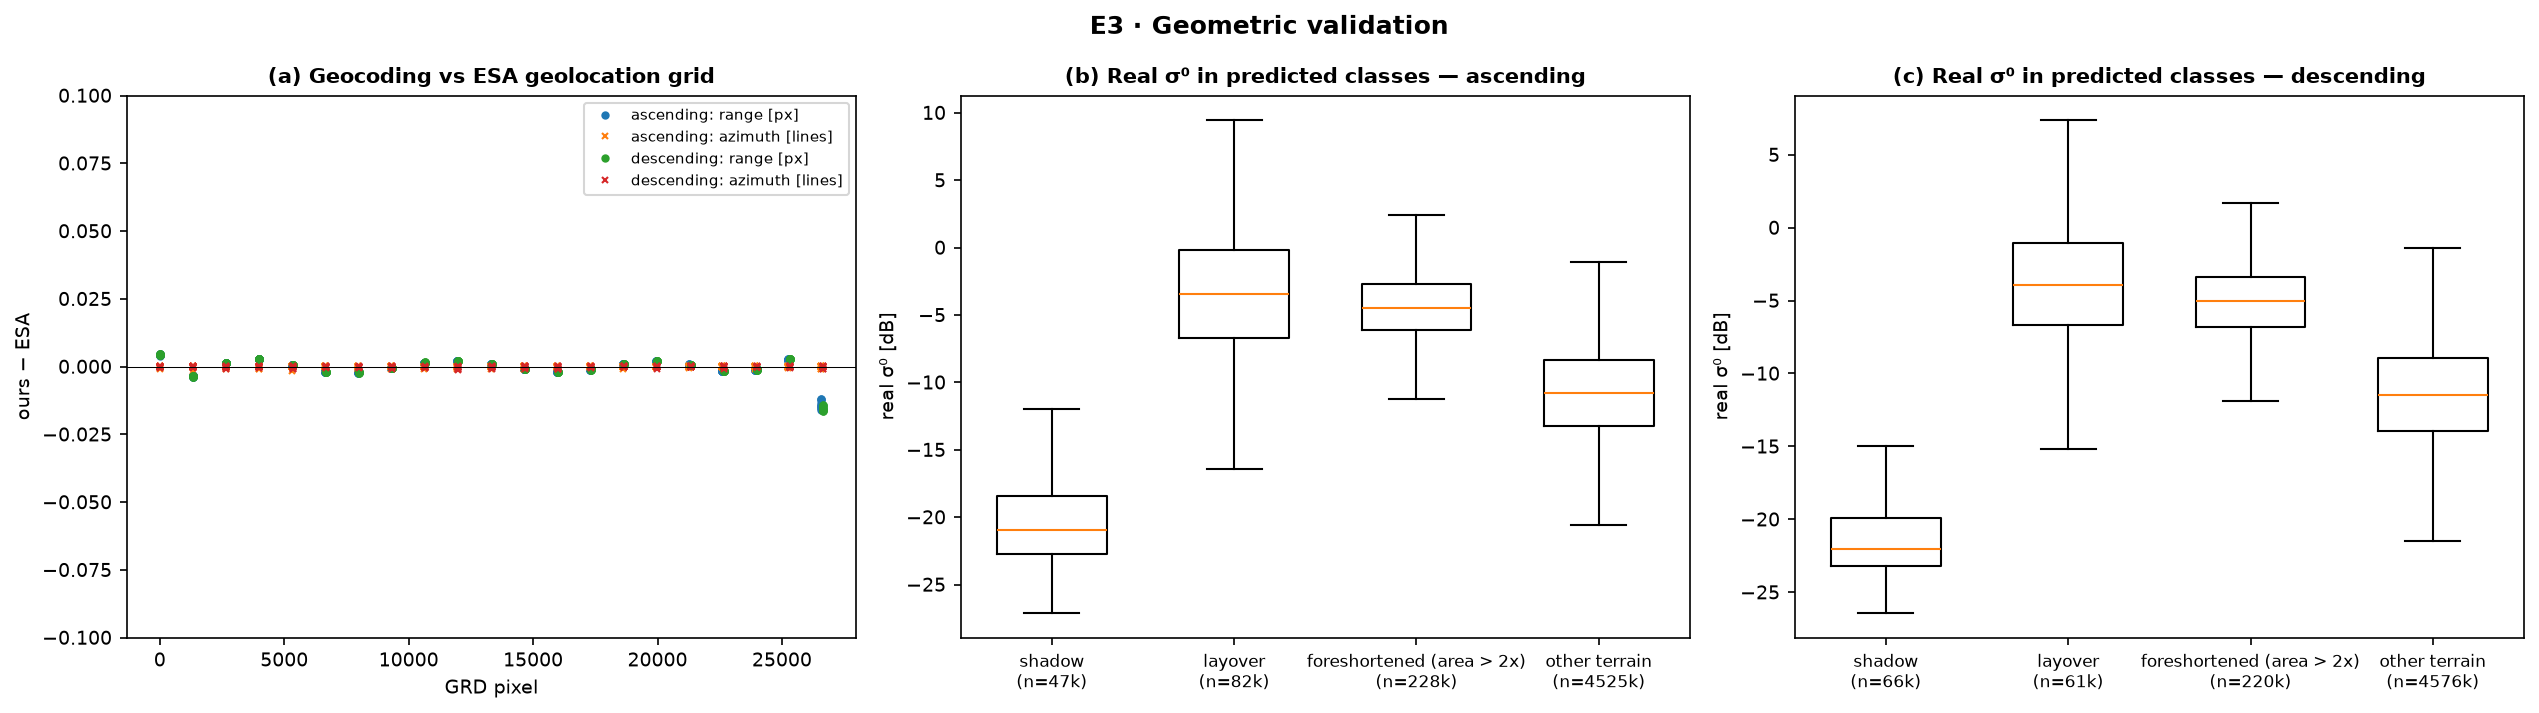
\includegraphics[width=\figw]{p4_geometric_validation.png}
\caption{Geometric validation: (\textbf{a}) geocoding residuals with respect to the geolocation grid of both products; (\textbf{b},\textbf{c}) real $\sigz$ in the predicted classes for the ascending and descending scenes.}
\label{fig:geomval}
\end{figure}

\subsection{Sensitivity to Processing Choices}
Table~\ref{tab:sens} and Figure~\ref{fig:sens} vary one processing choice at a time. Omitting the geoid correction ($N=\geoidN$\,m) moves the simulation by 5.8 pixels (58\,m) in range, in agreement with the expected ground-range displacement $N/\tan\theta$ of about 61\,m of a height error $N$ at an incidence angle of about 39$^\circ$; co-registration absorbs this shift and the correlation is unchanged, but an un-co-registered product such as a layover and shadow mask would be misplaced by six pixels. Without DEM oversampling, \holesNoOver\,\% of the GRD pixels receive no facet, compared with \holesBase\,\% with threefold oversampling, in a striped pattern on all slopes facing away from the radar. After $5\times5$ multilooking the correlation hardly changes ($r=\rNoOver$), but single-look products and masks would be unusable. A 90\,m DEM gives the same correlation as GLO-30 ($r=\rDemNinety$): at the 50\,m scale of the comparison, the large landforms dominate, and the finer DEM matters for full-resolution products.

\begin{table}[htbp]
\caption{Sensitivity of the simulation (ascending scene, fitted law). $\Delta$line and $\Delta$pixel are the residual shifts found by co-registration.}
\label{tab:sens}
\centering\small
\resizebox{\textwidth}{!}{\begin{tabular}{lrrrrr}\toprule
 Configuration & $r$ & SSIM & $\Delta$line & $\Delta$pixel & empty px [\%]\\\midrule
baseline (GLO-30, 3x oversampled, geoid) & 0.710 & 0.508 & -2.2 & 3.5 & 0.01 \\
no geoid correction (N = 0) & 0.710 & 0.507 & -2.2 & -2.3 & 0.01 \\
no DEM oversampling & 0.706 & 0.446 & -2.2 & 3.5 & 45.82 \\
90 m DEM (GLO-30 aggregated 3x3) & 0.714 & 0.418 & -2.3 & 3.5 & 0.00 \\
\bottomrule\end{tabular}
}
\end{table}
\begin{figure}[htbp]
\centering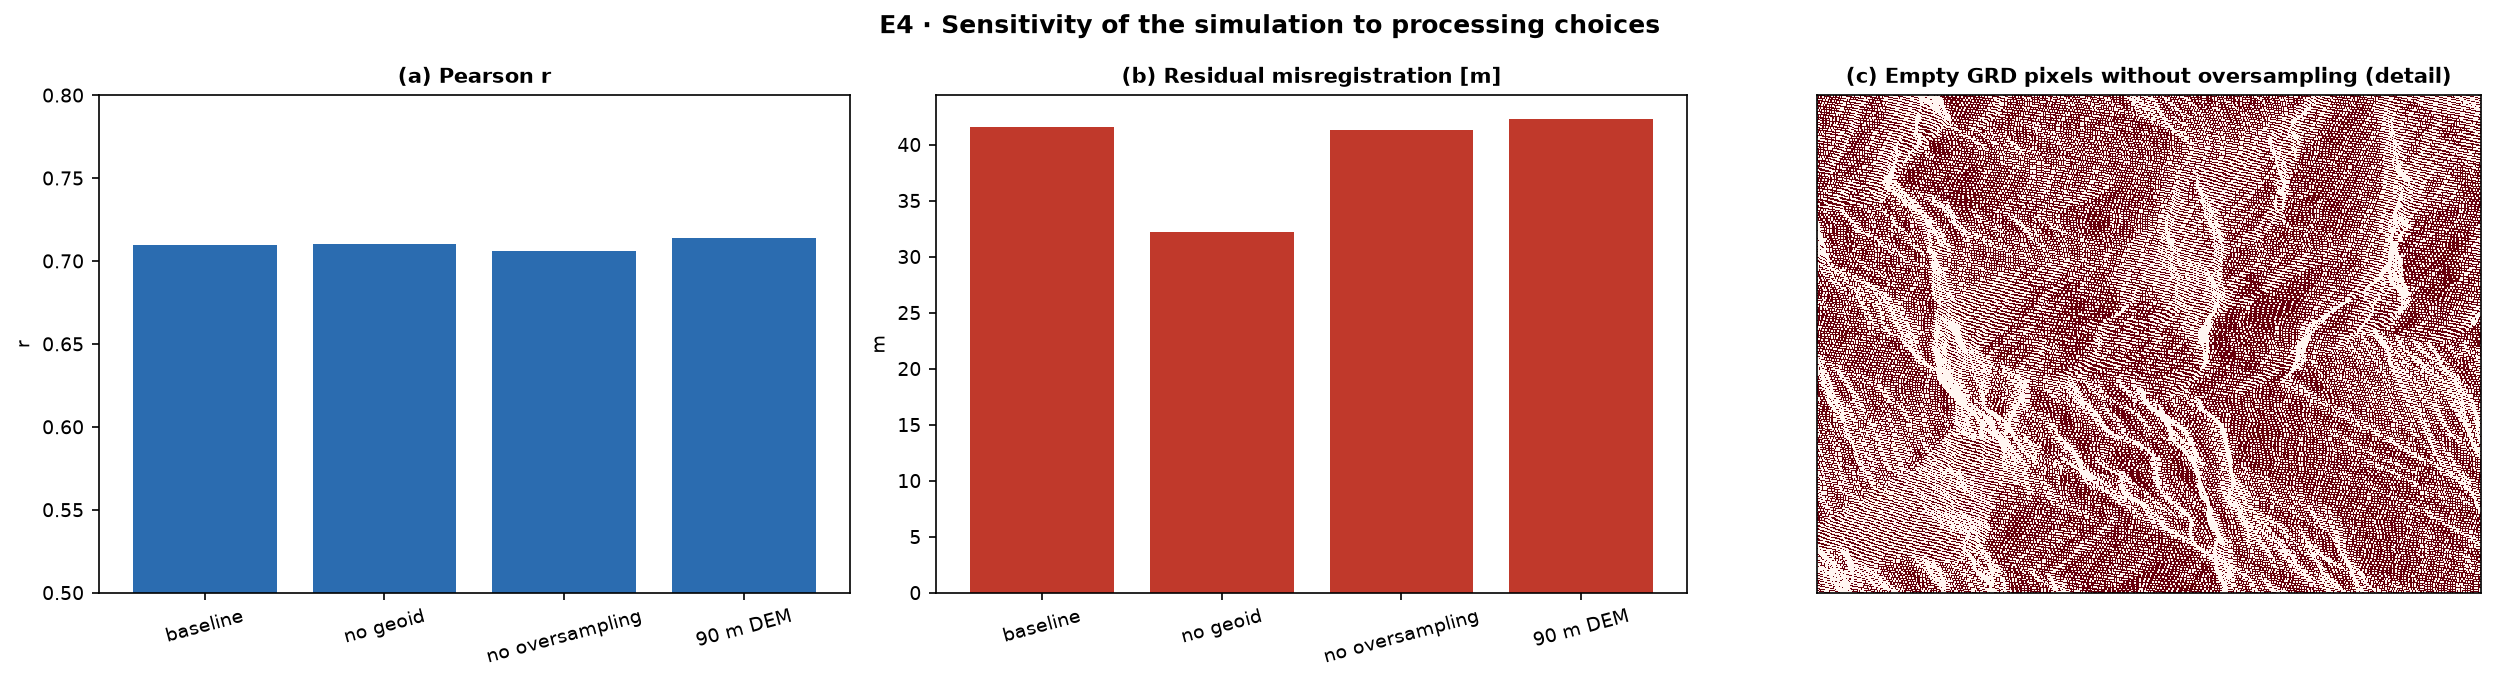
\includegraphics[width=\figw]{p5_sensitivity.png}
\caption{Sensitivity: (\textbf{a}) correlation; (\textbf{b}) residual misregistration; (\textbf{c}) GRD pixels that receive no facet without DEM oversampling (detail of the Nordkette).}
\label{fig:sens}
\end{figure}

\subsection{Contribution of Land Cover}
Grouping the residuals by WorldCover class (Table~\ref{tab:lc}, Figures~\ref{fig:lc} and~\ref{fig:resmap}) shows where a DEM-only simulation fails. Tree cover, which represents 55\,\% of the area, is reproduced without bias ($-0.1$\,dB) and with the highest correlation ($r=0.86$): the volume scattering of the forest canopy is close to the smooth angular law fitted to a scene that forest dominates. Built-up areas ($+3.1$\,dB) are brighter than predicted because double-bounce reflections between walls and the ground are absent from any facet model~\cite{balz2009,auer2010}; bare rock and scree ($+3.2$\,dB) are rougher than the average surface. Water ($-3.8$\,dB), cropland ($-2.0$\,dB) and grassland ($-1.4$\,dB) are darker because smooth surfaces reflect specularly away from the radar~\cite{ulaby1982}. The low correlations within the built-up, cropland and water classes ($r=0.22$--$0.30$) do not indicate a geometric failure: these classes lie on the flat valley floor, where the DEM predicts an almost constant value and the terrain signal to correlate with is weak.

\begin{table}[htbp]
\caption{Residual (real minus simulated $\sigz$) and correlation per land-cover class (ascending scene, map geometry, layover and shadow excluded).}
\label{tab:lc}
\centering\small
\begin{tabular}{lrrrr}\toprule
 WorldCover class & area [\%] & mean residual [dB] & std [dB] & $r$\\\midrule
Tree cover & 55.3 & -0.14 & 2.52 & 0.86 \\
Grassland & 25.9 & -1.44 & 3.28 & 0.77 \\
Cropland & 3.9 & -2.00 & 2.54 & 0.23 \\
Built-up & 7.2 & 3.11 & 4.54 & 0.22 \\
Bare / sparse & 5.8 & 3.18 & 4.29 & 0.82 \\
Snow \& ice & 0.3 & 2.09 & 2.91 & 0.86 \\
Water & 0.5 & -3.76 & 4.12 & 0.30 \\
Moss \& lichen & 1.2 & 0.51 & 3.27 & 0.88 \\
\bottomrule\end{tabular}

\end{table}
\begin{figure}[htbp]
\centering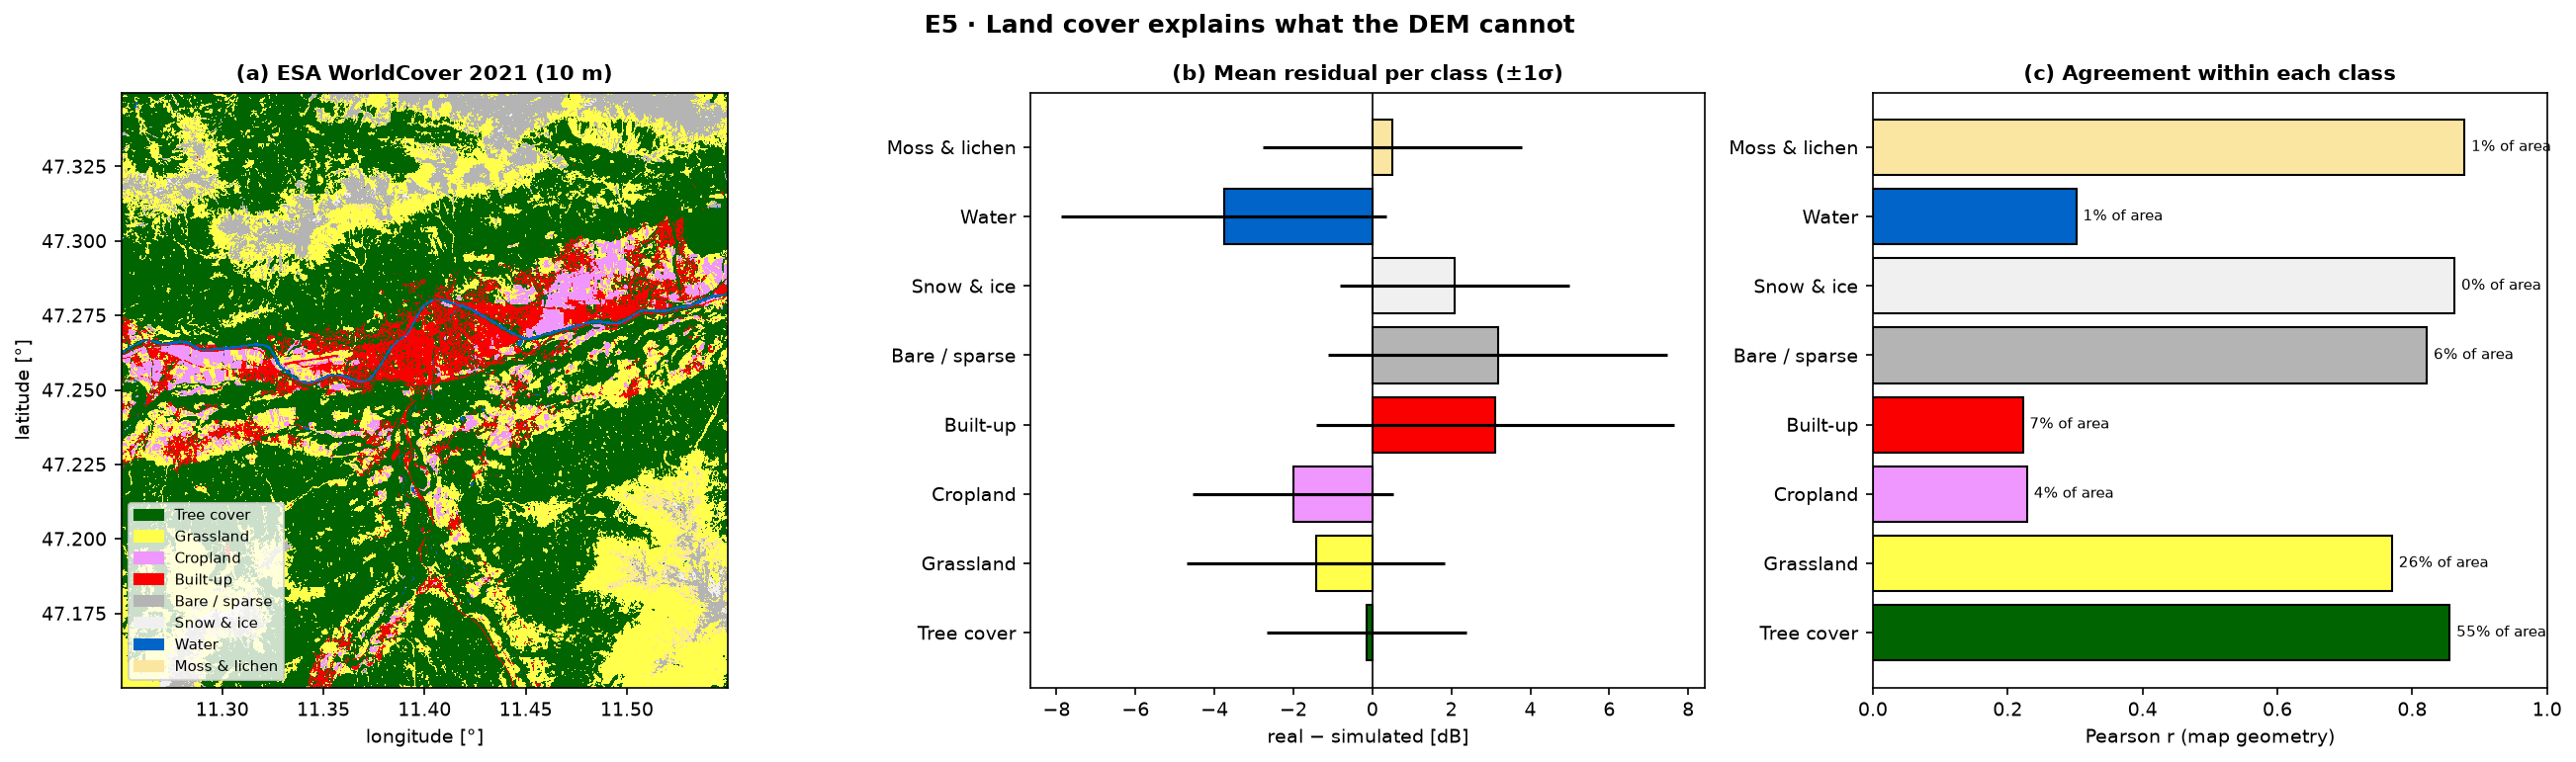
\includegraphics[width=\figw]{p6_landcover.png}
\caption{Land cover: (\textbf{a}) ESA WorldCover map of the study site; (\textbf{b}) mean residual per class ($\pm1$ standard deviation); (\textbf{c}) correlation within each class.}
\label{fig:lc}
\end{figure}
\begin{figure}[htbp]
\centering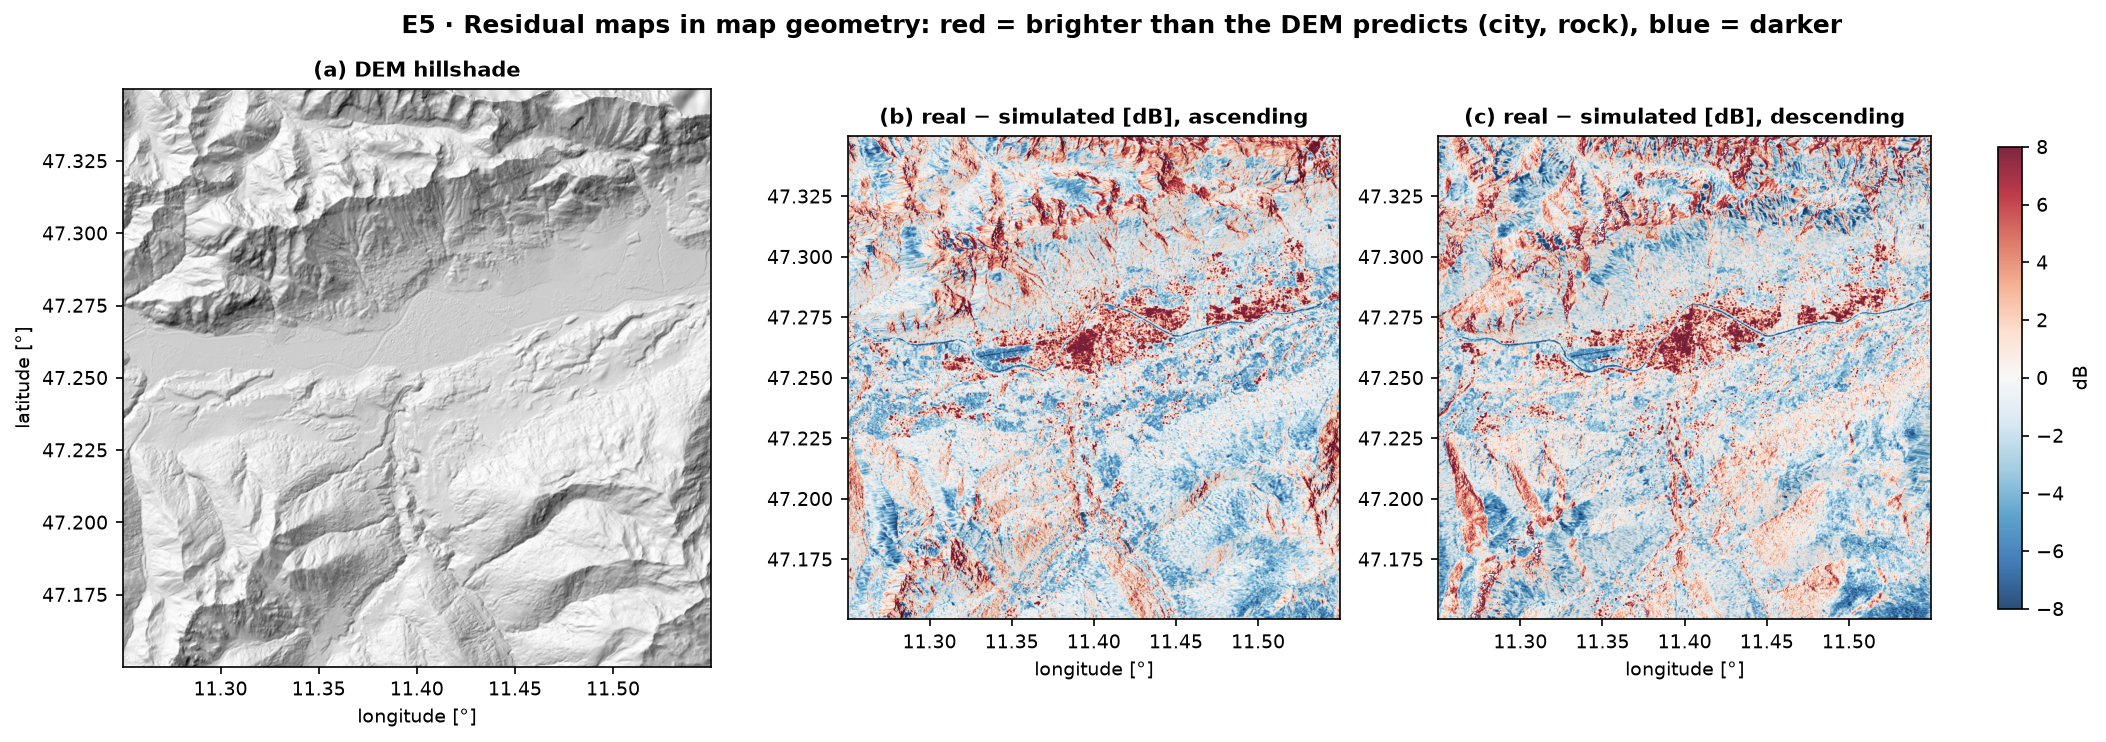
\includegraphics[width=\figw]{p7_residual_maps.png}
\caption{DEM hillshade (\textbf{a}) and residual maps (real minus simulated $\sigz$) in map geometry for the ascending (\textbf{b}) and descending (\textbf{c}) scenes.}
\label{fig:resmap}
\end{figure}

\subsection{Limitations of the Study}
The results presented in this section show that terrain geometry explains a large part of Sentinel-1 images of Alpine terrain. A few limitations related to the data and the methodology should nevertheless be discussed.

First, co-registration still finds offsets between image and simulation of \shiftAscL{} lines and \shiftAscP{} pixels (about 22\,m in azimuth and 35\,m in range) for the ascending scene and \shiftDescL{} lines and \shiftDescP{} pixels for the descending scene. Because the geocoding reproduces the product annotation to a small fraction of a pixel, these offsets measure the discrepancy between the image content and the annotated geolocation of the products, combined with DEM errors on steep slopes. Atmospheric path delay, solid-earth tides and the orbit used for near-real-time products, which are not modelled here, are known to contribute to the absolute geolocation error of Sentinel-1~\cite{schubert2015,gisinger2021}. Such offsets are routinely removed by simulation-based co-registration~\cite{nitti2011,small2011}.

Second, the simulator is an incoherent single-bounce model. It does not represent double bounce, volume scattering or multipath, which explains the residuals over built-up areas and the spread of real $\sigz$ at a given local incidence angle. Third, thermal noise was not removed, so that predicted shadow is compared with the noise floor rather than with zero. Fourth, one date per geometry was used; seasonal effects such as snow cover or soil moisture, and the time difference between the DEM acquisitions and the 2025 images, were not analysed. Finally, the absolute level of each backscatter law was calibrated by a constant; absolute radiometric prediction would require a land-cover-dependent model. These limitations do not affect the geometric conclusions of this study.

% ================================================================= 5
\section{Conclusions}
\label{sec:conclusions}
This study developed a SAR simulator from first principles and assessed how far a simulation driven only by a DEM and the annotated orbit of the product predicts real Sentinel-1 images of Alpine terrain. A raw-signal simulator, verified against theory from the impulse response of a point target to a real DEM, validated a fast image-domain simulator ($r=0.97$). Range-Doppler geocoding with the annotated orbit reproduced the geolocation grid of the products to \geoDpixMax{} pixels, provided that the slant-to-ground-range polynomials are applied piece-wise rather than interpolated; interpolation caused errors of up to 3.3 pixels. Predicted shadow and layover coincided with the darkest and brightest real pixels in both viewing geometries. A local-incidence-angle law $k\cos^{n}\theta_{loc}$ fitted to the ascending scene, with $n=\nFit$ (close to Lambert's law), reproduced the real $\sigz$ with $r=\rAsc$ and transferred unchanged to the descending scene ($r=\rDesc$). Geoid correction and DEM oversampling proved essential for products at full resolution, while a 90\,m DEM sufficed at the 50\,m scale of the comparison. The remaining disagreement is dominated by land cover: forest was reproduced without bias, whereas built-up areas and bare rock were about 3\,dB brighter and water about 4\,dB darker than predicted. Future work will introduce land-cover-dependent backscatter and double bounce, remove thermal noise, extend the analysis to multi-temporal stacks, and use the simulation for radiometric terrain flattening and automatic co-registration.

% ================================================================= BACK MATTER
\vspace{8pt}
{\small
\noindent\textbf{Author Contributions:} This work was carried out by Vedansh Shrivastava (Roll No.\ 230003086) as a B.Tech.\ minor project under the supervision of Dr.\ Unmesh Khati, Indian Institute of Technology Indore.

\vspace{4pt}\noindent\textbf{Data Availability Statement:} The code, the experiment pipeline, the tutorial notebook, the derived results and all figures are available at \url{\repoURL} (Appendix~\ref{app:code}). Copernicus GLO-30, Sentinel-1 GRD and ESA WorldCover data are openly available through the Microsoft Planetary Computer.

\vspace{4pt}\noindent\textbf{Acknowledgments:} The author thanks Dr.\ Unmesh Khati for his supervision and guidance. The Copernicus DEM is provided by ESA and Airbus; Sentinel-1 data and WorldCover are provided by ESA within the Copernicus Programme. Data access was provided by the Microsoft Planetary Computer.
\par}

\vspace{8pt}
{\small
\begin{thebibliography}{99}
\bibitem{torres2012} Torres, R.; Snoeij, P.; Geudtner, D.; Bibby, D.; Davidson, M.; Attema, E.; Potin, P.; Rommen, B.; Floury, N.; Brown, M.; et al. GMES Sentinel-1 mission. \textit{Remote Sens. Environ.} \textbf{2012}, \textit{120}, 9--24.
\bibitem{moreira2013} Moreira, A.; Prats-Iraola, P.; Younis, M.; Krieger, G.; Hajnsek, I.; Papathanassiou, K.P. A tutorial on synthetic aperture radar. \textit{IEEE Geosci. Remote Sens. Mag.} \textbf{2013}, \textit{1}, 6--43.
\bibitem{curlander1991} Curlander, J.C.; McDonough, R.N. \textit{Synthetic Aperture Radar: Systems and Signal Processing}; Wiley: New York, NY, USA, 1991.
\bibitem{cumming2005} Cumming, I.G.; Wong, F.H. \textit{Digital Processing of Synthetic Aperture Radar Data: Algorithms and Implementation}; Artech House: Norwood, MA, USA, 2005.
\bibitem{leberl1990} Leberl, F.W. \textit{Radargrammetric Image Processing}; Artech House: Norwood, MA, USA, 1990.
\bibitem{kropatsch1990} Kropatsch, W.G.; Strobl, D. The generation of SAR layover and shadow maps from digital elevation models. \textit{IEEE Trans. Geosci. Remote Sens.} \textbf{1990}, \textit{28}, 98--107.
\bibitem{gelautz1998} Gelautz, M.; Frick, H.; Raggam, J.; Burgstaller, J.; Leberl, F. SAR image simulation and analysis of alpine terrain. \textit{ISPRS J. Photogramm. Remote Sens.} \textbf{1998}, \textit{53}, 17--38.
\bibitem{schreier1993} Schreier, G. (Ed.) \textit{SAR Geocoding: Data and Systems}; Wichmann: Karlsruhe, Germany, 1993.
\bibitem{meier1993} Meier, E.; Frei, U.; N\"uesch, D. Precise terrain corrected geocoded images. In \textit{SAR Geocoding: Data and Systems}; Schreier, G., Ed.; Wichmann: Karlsruhe, Germany, 1993; pp. 173--185.
\bibitem{small2011} Small, D. Flattening gamma: Radiometric terrain correction for SAR imagery. \textit{IEEE Trans. Geosci. Remote Sens.} \textbf{2011}, \textit{49}, 3081--3093.
\bibitem{low2007} L\"ow, A.; Mauser, W. Generation of geometrically and radiometrically terrain corrected SAR image products. \textit{Remote Sens. Environ.} \textbf{2007}, \textit{106}, 337--349.
\bibitem{ulander1996} Ulander, L.M.H. Radiometric slope correction of synthetic-aperture radar images. \textit{IEEE Trans. Geosci. Remote Sens.} \textbf{1996}, \textit{34}, 1115--1122.
\bibitem{frey2013} Frey, O.; Santoro, M.; Werner, C.L.; Wegm\"uller, U. DEM-based SAR pixel-area estimation for enhanced geocoding refinement and radiometric normalization. \textit{IEEE Geosci. Remote Sens. Lett.} \textbf{2013}, \textit{10}, 48--52.
\bibitem{nitti2011} Nitti, D.O.; Hanssen, R.F.; Refice, A.; Bovenga, F.; Nutricato, R. Impact of DEM-assisted coregistration on high-resolution SAR interferometry. \textit{IEEE Trans. Geosci. Remote Sens.} \textbf{2011}, \textit{49}, 1127--1143.
\bibitem{franceschetti1992} Franceschetti, G.; Migliaccio, M.; Riccio, D.; Schirinzi, G. SARAS: A synthetic aperture radar (SAR) raw signal simulator. \textit{IEEE Trans. Geosci. Remote Sens.} \textbf{1992}, \textit{30}, 110--123.
\bibitem{balz2009} Balz, T.; Stilla, U. Hybrid GPU-based single- and double-bounce SAR simulation. \textit{IEEE Trans. Geosci. Remote Sens.} \textbf{2009}, \textit{47}, 3519--3529.
\bibitem{auer2010} Auer, S.; Hinz, S.; Bamler, R. Ray-tracing simulation techniques for understanding high-resolution SAR images. \textit{IEEE Trans. Geosci. Remote Sens.} \textbf{2010}, \textit{48}, 1445--1456.
\bibitem{muhleman1964} Muhleman, D.O. Radar scattering from Venus and the Moon. \textit{Astron. J.} \textbf{1964}, \textit{69}, 34--41.
\bibitem{ulaby1982} Ulaby, F.T.; Moore, R.K.; Fung, A.K. \textit{Microwave Remote Sensing: Active and Passive, Vol. II: Radar Remote Sensing and Surface Scattering and Emission Theory}; Addison-Wesley: Reading, MA, USA, 1982.
\bibitem{ulaby1989} Ulaby, F.T.; Dobson, M.C. \textit{Handbook of Radar Scattering Statistics for Terrain}; Artech House: Norwood, MA, USA, 1989.
\bibitem{copdem} European Space Agency; Airbus. \textit{Copernicus DEM: Global and European Digital Elevation Model (COP-DEM)}: Product Handbook; ESA: Paris, France, 2022.
\bibitem{s1pd} European Space Agency. \textit{Sentinel-1 Product Definition}; S1-RS-MDA-52-7440; ESA: Paris, France.
\bibitem{planetary} Microsoft. Planetary Computer. Available online: \url{https://planetarycomputer.microsoft.com} (accessed on 28 November 2026).
\bibitem{schubert2015} Schubert, A.; Small, D.; Miranda, N.; Geudtner, D.; Meier, E. Sentinel-1A product geolocation accuracy: Commissioning phase results. \textit{Remote Sens.} \textbf{2015}, \textit{7}, 9431--9449.
\bibitem{gisinger2021} Gisinger, C.; Schubert, A.; Breit, H.; Garthwaite, M.; Balss, U.; Willberg, M.; Small, D.; Eineder, M.; Miranda, N. In-depth verification of Sentinel-1 and TerraSAR-X geolocation accuracy using the Australian corner reflector array. \textit{IEEE Trans. Geosci. Remote Sens.} \textbf{2021}, \textit{59}, 1154--1181.
\bibitem{pavlis2012} Pavlis, N.K.; Holmes, S.A.; Kenyon, S.C.; Factor, J.K. The development and evaluation of the Earth Gravitational Model 2008 (EGM2008). \textit{J. Geophys. Res.} \textbf{2012}, \textit{117}, B04406.
\bibitem{worldcover} Zanaga, D.; Van De Kerchove, R.; Daems, D.; De Keersmaecker, W.; Brockmann, C.; Kirches, G.; Wevers, J.; Cartus, O.; Santoro, M.; Fritz, S.; et al. \textit{ESA WorldCover 10 m 2021 v200}; Zenodo, 2022. doi:10.5281/zenodo.7254221.
\bibitem{wang2004} Wang, Z.; Bovik, A.C.; Sheikh, H.R.; Simoncelli, E.P. Image quality assessment: From error visibility to structural similarity. \textit{IEEE Trans. Image Process.} \textbf{2004}, \textit{13}, 600--612.
\bibitem{goodman1976} Goodman, J.W. Some fundamental properties of speckle. \textit{J. Opt. Soc. Am.} \textbf{1976}, \textit{66}, 1145--1150.
\bibitem{oliver1998} Oliver, C.; Quegan, S. \textit{Understanding Synthetic Aperture Radar Images}; Artech House: Norwood, MA, USA, 1998.
\end{thebibliography}
\par}

% ================================================================= APPENDIX
\appendix
\section{Code and Data Availability}
\label{app:code}
\noindent\begin{minipage}{0.68\textwidth}
The \texttt{sarsim} package, the experiment pipeline \texttt{run\_all.py}, the unit tests, the tutorial notebook, this manuscript and the posters are available at\\[3pt]
\url{\repoURL}\\[3pt]
The environment is pinned with \texttt{uv} (Python 3.12). Every number and figure is reproduced by:
\begin{verbatim}
uv sync
uv run pytest -q tests
uv run python run_all.py
uv run python report/make_tables.py
\end{verbatim}
All input data are downloaded from the Microsoft Planetary Computer without registration and cached locally. Sentinel-1 products used:\\[2pt]
{\scriptsize\ttfamily \sceneAsc\\ \sceneDesc}
\end{minipage}\hfill
\begin{minipage}{0.27\textwidth}\centering

\includegraphics[width=\textwidth]{qr_repo.png}\\[2pt]
{\small Repository}
\end{minipage}

\section{Repository Structure}
{\small
\begin{tabularx}{\textwidth}{lX}\toprule
\texttt{sarsim/s1.py} & annotation parser, orbit fit, zero-Doppler geocoding, SRGR conversion, calibration\\
\texttt{sarsim/rdsim.py} & facet geometry, shadow and layover, backscatter laws, rendering\\
\texttt{sarsim/compare.py} & multilooking, co-registration, metrics, back-geocoding\\
\texttt{sarsim/data.py} & cached access to GLO-30, Sentinel-1 GRD windows and WorldCover\\
\texttt{run\_all.py} & experiments E1--E5; figures in \texttt{figures/pipeline/}, results in \texttt{results/}\\
\texttt{notebooks/} & tutorial notebook (executed \texttt{.ipynb} and jupytext \texttt{.py} source)\\
\texttt{tests/} & unit tests\\
\texttt{report/}, \texttt{poster/} & this manuscript, the A3 and A1 posters, Canva package\\
\bottomrule\end{tabularx}\par}
\end{document}
